\documentclass[a4paper,UKenglish]{modules/ifimaster}
%\documentclass[UKenglish]{modules/ifimaster}  %% ... or USenglish or norsk or nynorsk
\usepackage[utf8]{inputenc}           %% ... or latin1 or applemac
\usepackage[T1]{fontenc,url}
\urlstyle{sf}
\usepackage{babel,textcomp,csquotes,modules/duomasterforside,varioref,graphicx}
%\usepackage[backend=biber,style=numeric-comp]{biblatex}
\usepackage{modules/masterfrontpage,amsmath}
\usepackage{booktabs}
\usepackage{subcaption}
\usepackage{natbib}
%\bibliographystyle{unsrtnat}
\bibliographystyle{apalike}


%\addbibresource{tex/refs.bib}

\author{Cyril Antille - \today}
\title{The effect of tissue motion on multibeam Iterative Adaptive Approach beamforming in medical ultrasound imaging}

\begin{document}
    \masterfrontpage
    
    %\duoforside[dept={Department of Informatics},   %% ... or your department
    %  program={Network and system administration},  %% ... or your programme
    %  short]                                        %% ... or long
    
    \frontmatter{}
    %\par\vspace*{.35\textheight}{\centering Dedicated to someone special\par}
    \chapter*{Acknowledgement}

I would like to thank my supervisors Associate Professor Are Jensen and Professor Andreas Austeng for offering me such an interesting thesis topic and for their incredible support during its development.
This thesis was not always easy to conciliate with a time-consuming and challenging job, but Are and Andreas have both been extremely patient and understanding with my situation.

Besides their contribution to this thesis, they, along with Professor Sverre Holm, have introduced me to the DSB research group and have always encouraged me to join their seminars and events. I sincerely congratulate them, and every member of the DSB group, for maintaining such an excellent atmosphere and will of mutual help within that group.

When I joined UiO for a Master program, Andreas gave me precious advice about the structure of my program, from the choice of courses to the topic for Master thesis. I also owe my current job position to Andreas' and Sverre's courses and their relationship with industries in related domains.

I would also like to thank my parents for their moral and financial support and for encouraging me to challenge myself and take risks.
Finally, thanks to Mary for her patience during those long days, and nights, of work.
    
\chapter*{Abstract}
Conventional 2D medical ultrasound imaging is based on analyzing the backscatter 
(echoes) from multiple, focused, transmitted acoustic beams.
Most imaging systems are very similar in the way they create and record beams. Their main difference comes from their analysis of the recorded data.
Adaptive beamformers have been introduced in the 60s as high-resolution beamformers and are still extensively researched to this day. Such beamformers are, in the best case, able to achieve higher resolution than conventional ones. They are however often less reliable, more computationally complex and less intuitive to use, which is why conventional beamformers are often preferred in commercial products.

Traditionally, ultrasound images are created by transmitting beams in various directions and, for each beam, create image samples along its trajectory.
Often, however, there is a large overlap between the areas covered by the respective beams.
This phenomena can be used to achieve higher spatial resolution by creating image samples based on multiple beams instead of a single one.
Beamformers that use multiple beams per image sample are often referred to as \textit{multibeam} beamformers, as opposed to the traditional \textit{singlebeam} beamformers.
Some approaches to multibeam beamforming have shown to result in increased ability to resolve scatterer points over their singlebeam counterpart, as well as increased robustness to noise for adaptive beamformers (\cite{Jensen_multibeam}).
Although those results are very promising, they only cover scenarios where the imaged medium is stationary.
The primary goal of this thesis is to discover how multibeam beamformers handle tissue motion.

\cite{Asen_shift_invariance} showed that singlebeam beamforming in the presence of tissue motion may result in visible amplitude variations of the scatterer points in motion. The amplitude variations are caused by an effect known as scalloping loss. If those variations are kept below a given visibility threshold, the beamformer is said to be lateral shift-invariant.
\cite{Asen_shift_invariance} showed that singlebeam beamformers can be made lateral shift-invariant by setting a sufficiently high density of transmit and receive beams.
We confirm those results in this thesis and find that this approach also works with multibeam beamformers.

However, a beamformer's image acquisition time, and therefore frame rate, is directly influenced by its transmit beam density.
Many applications have minimum frame rate requirements, especially real-time imaging applications. This limitation on the transmit beam density may in some applications be too strict to guarantee lateral shift-invariance of a beamformer.
Furthermore, we show that tissue motion can cause shape distortion of scatterer points in addition to potential amplitude variations, and that the magnitude of this effects increases proportionally with image acquisition time.

A commonly-used approach to reducing image acquisition time while retaining high resolution 
is parallel-receive beamforming (PRB), also known as multiple-line acquisition (MLA).
The principle is to allow relatively low transmit beam densities by angular oversampling of the receive beams. However, again due to transmitting and receiving focused beams, receive beams that are not aligned with transmit beams can experience scalloping loss.
Multiple MLA approaches have been explored, some of which trying to correct for scalloping loss (\cite{prb_approaches}).
In this thesis, perfect MLA is first used and simulated by running the standard single-beam acquisition (SLA) with angular oversampling on transmit beams as well as receive beams.
Then a naive approach to MLA, without correction for scalloping loss, is implemented and its sensitivity to tissue motion compared to that of perfect MLA.
We show that naive MLA is more sensitive to scalloping loss than perfect MLA at low beam densities, but its sensitivity converges towards that of perfect MLA with increasing transmit beam densities.

The conventional DAS beamformer and the adaptive MV beamformer are well known in the medical ultrasound domain and often taken as standards of comparison in academical studies.
In order to build confidence in our results for multibeam beamformers, the same experiments and analyses are done with the singlebeam DAS and MV beamformers. This also provides a common base with existing studies.
The multibeam beamformers used in this thesis are using the Iterative Adaptive Approach (IAA), which has recently been presented as an alternative adaptive beamforming technique (\cite{Yardibi}).
\cite{Jensen_IAA} showed that multibeam IAA can achieve similar scatterer points resolvability as MV while being more robust than MV to signal cancellation.

Several implementations of the IAA exist, so we chose to focus on variants of the IAA beamformer both based on the multibeam covariance matrix estimate and multibeam output (MB) approach (\cite{Jensen_IAA}) during the iteration process.
In this thesis, we refer to those beamformers as IAA-MB beamformers.
The variants of IAA-MB implemented in this thesis only differ in their final step of the creation of a beamformed image sample; one variant based on the MB approach (IAA-MBMB) and the other based on the singlebeam output (SB) approach (IAA-MBSB).

We confirm the results from \cite{Jensen_IAA} with the IAA-MB beamformers for static imaged media, but show that the presence of tissue motion can induce distortions that reduce the scatterer point resolvability of the multibeam IAA beamformers below that of MV.
In extreme cases, the resolvability of IAA-MBMB can even become worst than that of DAS.
However, we also show than MLA can be used to reduce the distortion effects and maintain high resolvability capacities.
Furthermore, the IAA-MBMB beamformer impressively corrects for the receive beams misalignment induced by MLA and yields similar performances with naive MLA than with perfect MLA.

Although multibeam beamformers are by nature more sensitive to tissue motion than singlebeam ones, we show that, with an appropriate use of the MLA technique, the IAA-MB beamformers can be made lateral shift-invariant and robust to motion-induced distortion.
We think that the multibeam IAA beamformers can globally be made as robust and easy to use as the conventional DAS beamformer, while maintaining high resolution and frame rate capacities.

          % include the abstract
    
    \tableofcontents{}
    \listoffigures{}
    \listoftables{}
    
    \mainmatter{}
    \chapter{Introduction}

Medical ultrasound imaging is a non-invasive technique that provides a visual representation of internal body elements. It typically consists of using a probe to transmit directional beams and record their echoes backscattered from the imaged body elements. 
Beams are physically created from multiple transducers sending the same signal pulse with different time delays in order to result in constructive interference at a given point of focus and hopefully in destructive interference in other directions.
A similar approach is done on the recorded data. Given a point of focus, the data recorded by each transducer can be time-delayed such that potential signals coming from that focus point are aligned and can be added up coherently if summing the data recorded by all transducers.

The algorithms used for beam transmission and recording are mostly referred to as \textit{beamformers}. In medical ultrasound imaging, many beamformers have been proposed over the years. Most of them work in the same way for beam transmission and recording, but the major difference between them comes from how the recorded data is combined.
Given the set of data recorded by all transducers after a beam transmit, each transducer can be given a different time-delay and amplitude weight values.
Conventional beamformers work very similarly to parabolic dishes for antennas. A pre-defined set of amplitude weights and time delays defines the \textit{aperture} of the array, which in that analogy corresponds to the shape of the parabolic dish. The set of time delays also defines the focus point of the array. The major advantage of digital beamformers over parabolic dishes is that they are not constrained to a single physical shape and focus point. A digital array has the ability to have simultaneously multiple focus points on reception simply by assigning different sets of time delays to the same recorded data.
The Delay-And-Sum (DAS) beamformer is a conventional beamformer that, as its name indicates, simply builds an image sample by time delaying the recorded data to focus the array towards the corresponding position and sum the time-delayed data. This algorithm is conceptually and computationally simple, very reliable and still very much used to this day. For those reasons, it is the beamformer of reference for many studies and this thesis is no exception.

Another major type of digital beamformers, often referred to as \textit{adaptive} beamformers, emerged in the 60s as 'high-resolution' beamformers (\cite{Capon}). Their main difference with conventional beamformers is that, instead of using pre-defined amplitude weights, adaptive beamformers have the ability of adapting their aperture to the perceived wavefield. This ability allows the beamformers to generally form narrower receive beams and achieve higher resolution than conventional beamformers. Such beamformers are however generally less reliable, more computationally complex and less intuitive to use than conventional beamformers.
Some of the early concerns such beamformers faced included their notable sensitivity to:
\begin{enumerate}
    \item Signal cancellation in the presence of coherent signals (\cite{van_trees})
    \item Visible artifacts in the presence of motion in the imaged medium (\cite{Asen_shift_invariance})
    \item High beam density requirements due to narrow receive beams
    \item High computational complexity prohibiting real-time ultrasound imaging
    \item High configuration complexity
\end{enumerate}
\noindent
High-resolution beamformers have been, and still are, a great source of academical interest as possible alternative to the widely used conventional beamformers. 
In industry, they have however for a long time mainly been used in passive systems, where transducers do not transmit signals, but record potential signals from sources in the imaged medium. The main reason that adaptive beamformers were not much used in active systems is due to their sensitivity to coherent signals.
Their use in medical ultrasound imaging only started in beginning of the 2000s and a majority of commercial ultrasound imaging systems still prefer conventional beamformers to the adaptive ones.

One of the oldest and most known adaptive beamformers is the Capon, also known as minimum variance distortionless response (MV or MVDR), beamformer introduced by \cite{Capon}.
Different approaches have been proposed over time to solve or limit the effects of one issue or another.
In this thesis, some of those MV improvements are retraced and used.

An alternative approach to adaptive beamforming known as the Iterative Adaptive Approach (IAA) has recently been introduced to ultrasound imaging (\cite{Jensen_IAA}).
IAA has shown to yield promising results concerning high resolution capability and low configuration complexity. It has however only been studied with stationary images so far. This thesis aims to explore the effects of tissue motion on the IAA approach and compare its performances to the DAS and Capon beamformers regarding the for-mentioned concerns for adaptive beamformers.

The theoretical goal of forming directional beams is to radiate energy towards a specific point or direction without radiating energy towards other directions. In practice, it is not possible to do it perfectly due to the omnidirectional nature of wave propagation. This means that, for a single transmit beam, the recorded wavefield does not only hold information about potential scatterer points at the transmit beam focus point, but also in other directions.
A lot of beamformers treat this energy leakage as noise and typically build image samples based on their nearest transmit beam trajectory. Such beamformers are often referred to as \textit{singlebeam} beamformers.
Another approach to building image samples is to combine the information contained in multiple beams and use this energy leakage to that purpose.
The beamformers based on this approach are often referred to as \textit{multibeam} beamformers.

Both conventional and adaptive beamformers can be implemented as multibeam beamformers. The IAA beamformers used in this thesis are built as multibeam beamformers. Their performances with the presence of motion in the imaged medium are compared to those of the DAS and MV beamformers. Both DAS and MV are implemented as singlebeam algorithms in order to provide results and analysis comparable to existing studies.


Tissue motion in ultrasound imaging is not a new concept and is known to possibly cause visible artifacts in the beamformed images. \cite{Asen_shift_invariance} showed with the MV beamformer that lateral motion of elements in the imaged medium can result in their apparent amplitude or size varying from frame to frame. This effect is caused by angular undersampling and can potentially result in medium elements, or scatterer points, to visibly appear or disappear from one frame to another.
One of our main objective is to provide a similar analysis on the IAA beamformers, as well as for the DAS and MV beamformers for comparison.

A scatterer point's motion is often seen as merely a shift in its position from one frame to another. This representation would be accurate if the image acquisition of a single frame was instantaneous.
Obviously image acquisition is not instantaneous, which means that tissue motion can potentially induce artifacts within a single frame as well.
That is one aspect of motion that multibeam beamformers are expected to be more sensitive to than singlebeam beamformers, since they combine information from multiple, and potentially all, transmit beams for every image sample.

In this thesis, we analyze the effects of motion both within and between frames.
Even though the analysis done on the IAA beamformers is the most novel part of the thesis, we chose not to solely focus on them, but to pay equal attention to the DAS and MV beamformers. We believe that this approach provides a major confidence factor to the novel results and a very instructive journey into ultrasound imaging in general.

Chapter \ref{chap:background} provides a short introduction to ultrasound imaging and its applications in the medical domain.
After some necessary explanations on signal propagation and the concept of beamforming, it gives a presentation of conventional and adaptive beamforming along with several robustification methods.
Each of the beamformers used in this thesis are presented and thoroughly explained in this chapter.

All the experiments done in this thesis are simulations run in MATLAB with the \textit{Field II Simulation Program} (\cite{Field_II,Field_II_ext}).
Chapter \ref{chap:material} describes how the simulations are made and presents the choice of parameters for the simulated ultrasound probe, imaged medium and beamformers used.

Chapter \ref{chap:experiments} presents the experiments run in this thesis and their expected output.
Chapter \ref{chap:results} contains the results of those experiments along with our analysis of those results.
Since a lot of our experiments are heavily correlated, and some experiments require the analysis of other ones, we have chosen to merge our results and discussion of those into a single chapter.
Finally, Chapter \ref{chap:conclusion} provides a short summary of our findings as well as a few ideas for possible continuations of this thesis.


    \chapter{Background}
\label{chap:background}

This chapter provides a short introduction to ultrasound imaging in general and its use in the medical domain in particular. It then moves on to basic explanations on wave propagation, before moving deeper into the concept of \textit{beamforming}.
The excellent book 'Array Signal Processing - Concept and Techniques' by \cite{Dudgeon_book} has been a valuable source of information for this chapter.

Once the concept of conventional beamforming is thoroughly explained, this chapter builds on this theory to introduce the concept of \textit{adaptive beamforming} and presents different algorithms using that concept.
Most of the theory is first presented as broadly as possible, then narrowed down specifically to standard medical ultrasound imaging applications.


\section{Ultrasound imaging}
\label{sec:ultrasound_imaging}
Ultrasound imaging, also known as sonography or ultrasonography, is an imaging technique based on acoustic waves at frequencies above those audible by humans. It relies on the use of beamforming (Section \ref{sec:beamforming}) to give a spatial meaning to the recorded signals time and amplitude information. The frequency ranges used in ultrasound imaging vary depending on the application, but typically lie between $20~$kHz and $20~$MHz. This technology is used in multiple fields, some of the biggest being sonar (\cite{sonar}) and medical (\cite{medical_physics}).
Most ultrasound imaging systems can be classified into two groups:
\begin{itemize}
\item Passive: The system listens for sound waves emitted by sources in the zone of interest.
\item Active: The system emits sound waves and listen to echoes coming from the zone of interest.
\label{item:systems}
\end{itemize}

\subsection{Medical ultrasound imaging}
In the medical domain, ultrasound imaging is typically used as a noninvasive diagnostic tool to image body structures, such as organs or tissue. Ultrasound imaging systems are relatively cheap and portable, which makes them more accessible than the other imaging methods presented in Section \ref{sec:medical_imaging}.
Another advantage of ultrasound imaging is its ability to capture and process data in real-time, thus allowing real-time image analysis.
It is also considered safer than X-ray imaging, since it is based on non-ionizing radiation.
Besides its ability to image body elements, it can also be used to estimate blood flow velocities in arteries or vessels by analyzing the Doppler effect of backscattered signals (\cite{doppler_ultrasound}). The term 'Doppler ultrasound imaging' is then often used.

Since most, if not all, body structures do not emit acoustic waves, active imaging systems have to be used. A probe consisting of multiple transducers is typically pressed against the skin of the patient, and pointed towards the zone of interest, for example his/her heart, as illustrated in Figure \ref{fig:echocardiography}.

\begin{figure}[ht]
    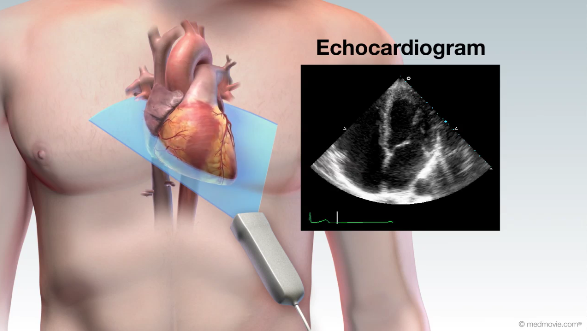
\includegraphics[width=\linewidth]{./images/background/echocardiogram.png}
	\caption{Illustration of ultrasound echocardiography (medmovie.com)}
	\label{fig:echocardiography}
\end{figure}

\subsection{Medical imaging}
\label{sec:medical_imaging}
Medical imaging refers to non-invasive techniques, unlike surgery, that provide a visual representation of internal body elements. Various imaging techniques exist, some of the most used ones being Magnetic Resonance Imaging (MRI), X-ray, Nuclear and Ultrasound. 
The choice of imaging technique depends on the the body part of interest and the diagnostic purpose. Table \ref{table:medical_imaging} shows a non-exhaustive comparison of those methods.

\begin{table}[!ht]
\centering
\begin{tabular}{| c || c |}
 \hline\hline
    &   Spatial resolution [mm] \\
  \hline
  Ultrasound    &   1 - 5 \\
  X-Rays    &   0.1 \\
  MRI   &   0.3 - 1 \\
  Nuclear   &   5 - 15 \\
  
  \hline\hline
    &   Safety \\
  \hline
  Ultrasound    &   No known hazards \\
  X-Rays    &   Small radiation dose \\
  MRI   &   Pacemakers and implants can be a hazard \\
  Nuclear   &   Moderate radiation dose \\
  
  \hline\hline
    &   Bone imaging \\
  \hline
  Ultrasound    &  Poor - Ultrasound does not penetrate bone \\
  X-Rays    &   Preferred technique \\
  MRI   &   Gives weak MRI signal \\
  Nuclear   &   Good for early diagnosis \\
  
  \hline\hline
    &   Heart and circulation imaging \\
  \hline
  Ultrasound    &  Preferred technique \\
  X-Rays    &   Needs contrast medium \\
  MRI   &    Good resolution capabilities \\
  Nuclear   &   Useful for flow studies \\
  \hline\hline
  
    &   Soft tissues imaging    \\
  \hline
  Ultrasound    & Preferred technique for areas with low bone density \\
  X-Ray &   Poor \\
  MRI   &   Preferred technique for muscles and joints \\
  Nuclear   & Poor \\
  \hline\hline
  
    &   Chest imaging   \\
  \hline
  Ultrasound    & Poor - Ultrasound can not image past air spaces \\
  X-Ray & Preferred technique for lung screening \\
  MRI   & Not good for imaging air spaces \\
  Nuclear   & Very good for air and blood flow imaging \\
  
  \hline\hline
  
    &   Brain and spinal cord imaging   \\
  \hline
  Ultrasound  & Poor - Difficult to image through skull \\
  X-Ray & Limited use \\
  MRI   & Preferred technique \\
  Nuclear   & Poor \\
  \hline
 \end{tabular}
\caption{Comparison of some of the main medical imaging techniques taken from 'Medical Physics: Imaging' by \cite{medical_physics}}
\label{table:medical_imaging}
\end{table}

\subsection{Therapeutic medical ultrasound}
Ultrasound is most widely used in the medical domain as a noninvasive diagnostic tool. It can however also be used for therapeutic applications. Ultrasound waves have been proven to cause local heating of tissue and increase in blood flow if radiating high levels of energy. It can also produce cavitation in extreme cases.
Ultrasound probes used for medical imaging are subject to strict restrictions in order to avoid or limit such effects. The use of such probes are therefore most of the time painless and completely harmless to the patient.

The potential side-effects of the use of ultrasound have however shown to be useful when used wisely. They gave birth to several therapeutic applications of ultrasound, such as targeted ultrasound delivery, high intensity focused ultrasound or lithotripsy, which is a procedure that uses shock waves to break up stones in the kidney, bladder, or ureter (\cite{lithotripsy}).

\section{Signal propagation and acquisition}
\label{sec:signals}

\subsection{Acoustic waves}
\label{sec:physics_waves}
A wave is an oscillation transferring energy in space without, or with little, transfer of mass. There are two main types of waves: \textit{Mechanical}, which can only propagate in a medium, and \textit{Electromagnetic}, which can propagate in vacuums as well.
\par
Ultrasound waves, and acoustic waves in general, are mechanical waves.
There exist two basic types of wave motion for mechanical waves: \textit{Longitudinal} and \textit{Transverse}. As shown in Figure \ref{fig:wave_types}, a longitudinal wave (P-wave) propagates through compression and dilatation along its direction of propagation, whereas a transverse wave (S-wave) propagates through oscillation of particles orthogonal of its direction of propagation.
In ultrasound medical imaging, the probe's transducers are oscillated in order to create pressure variations, and therefore longitudinal waves, in the imaged medium.
It is worth mentioning that transverse waves may be induced in that process and can be used in specific domains such as elastography.
However, in conventional ultrasound medical imaging, transverse waves are often ignored and therefore fall out of the scope of this thesis.

\begin{figure}[ht]
    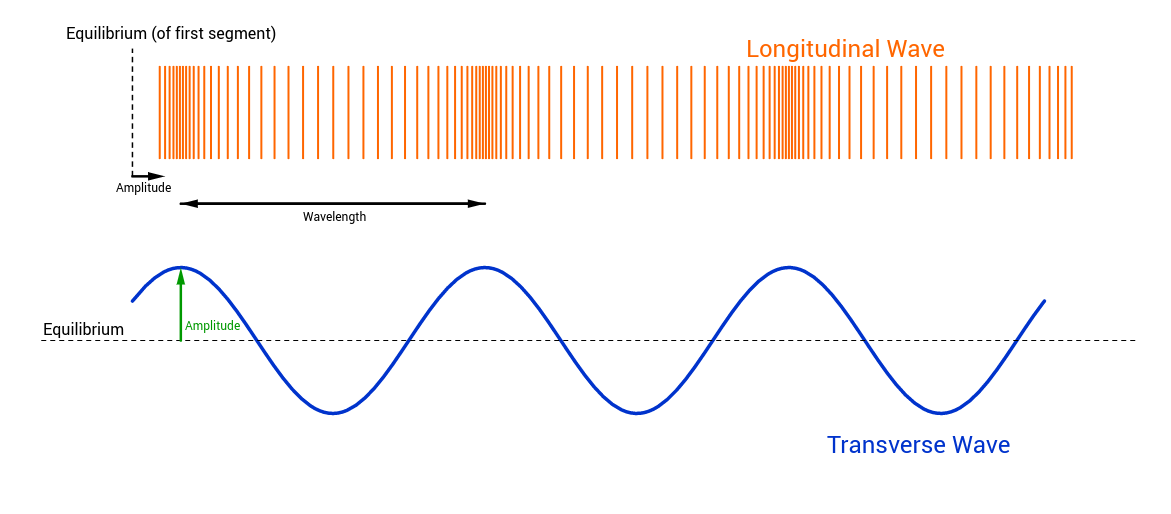
\includegraphics[width=\linewidth]{./images/background/wave_propagation.png}
	\caption{Longitudinal and transverse waves propagation. Illustration generated with \cite{wave_propagation}}
	\label{fig:wave_types}
\end{figure}


\subsection{Propagating waves}
\label{sec:prop_waves}
Information can be transmitted from one transducer to another by the means of propagating waves. The actual physics of the propagation depends on the type and properties of the wave and of the medium in which it propagates. Luckily a single formula can be used both for electromagnetic waves and acoustic waves. The lossless wave equation describes the propagation of a waveform $s(\boldsymbol{x}, t)$ in an ideal medium:
\begin{equation}
    \nabla^2 \boldsymbol{s} = \frac{\delta^2 \boldsymbol{s}}{\delta x^2} + \frac{\delta^2 \boldsymbol{s}}{\delta y^2} + \frac{\delta^2 \boldsymbol{s}}{\delta z^2} = \frac{1}{c^2} \frac{\delta^2 \boldsymbol{s}}{\delta t^2},
\end{equation}
\noindent
where $\boldsymbol{x} = (x, y, z)$ is the three dimensional spatial variable, $t$ the time variable, $\nabla^2$ is the Laplacian operator and $c$ the wave's speed of propagation. An ideal medium is a medium that does not induce any disturbance to the propagation of the wave, such as dispersion, refraction or attenuation. The lossless wave equation can easily be derived from Maxwell's equations for electromagnetic waves. For acoustic waves, the same equation can be built from fundamental physics principles (conservation of mass, equation of state, Newton's second law of motion). The derivation of the wave equation is however much more complicated for acoustic wave due to the fact that there is no unified set of equations, such a Maxwell's equations, defining all acoustic waves. The proof of the lossless wave equation is not provided in this thesis.

For electromagnetic waves, $c = \sqrt{\epsilon \mu}$, where $\epsilon$ is the medium's dielectric permittivity and $\mu$ is its magnetic permeability. For acoustic waves, $c$ is dependent on the medium's pressure and density.
As a rule of thumb, electromagnetic waves typically propagate at speeds in the order of $10^8 ~ m/s$  ($3 \cdot 10^8$ in free space) whereas acoustic waves propagate much slower, typically in the order of hundreds or thousands of m/s.

A monochromatic wave is a wave composed of a single frequency $\omega$. Such a wave can be described in the time domain as a complex exponential of frequency $\omega$:
\begin{equation}
    s(\boldsymbol{x},t) = A e^{j \omega t + \phi},
\label{eq:mono_wave}
\end{equation}
\noindent
where $A$ is a real or complex valued amplitude factor and $\phi$ is a phase delay dependent on $\boldsymbol{x}$.
Assuming that $\phi = 0$ at $x_0 = (0, 0, 0)$ and $\boldsymbol{x}$ is at distance $D = |\boldsymbol{x}|$ from $x_0$, the phase delay $\phi$ is then $\phi = \omega D / c$, where $c$ is the wave's speed of propagation

The theory presented in this section focuses on monochromatic waves, but Equation (\ref{eq:mono_wave}) can be extended to nonmonochromatic waves by applying the superposition principle:
\begin{equation}
    s(\boldsymbol{x},t) = \sum_{i=1}^I A_i e^{j \omega_i t + \phi_i},
\label{eq:superpos}
\end{equation}
\noindent
where $I$ is the length of the set $\Omega = [\omega_1, ..., \omega_I]$ of frequencies present in $s(\boldsymbol{x},t)$.
In practice, $\Omega$ is often an infinite set and Equation (\ref{eq:superpos}) is approximated with a finite set of frequencies.

Although waves are fundamentally considered as \textit{spherical} waves, they can sometimes be approximated to \textit{plane} waves.
Whereas spherical waves propagate in all directions, a plane wave can be seen as propagating in a single direction $\boldsymbol{\zeta}$.
Its phase delay can then be defined as $\phi = \omega \boldsymbol{\zeta} \cdot \boldsymbol{x} / c$.
The wave's propagation speed $c$ and direction $\boldsymbol{\zeta}$ are often combined into the wave's slowness vector $\boldsymbol{\alpha} = \boldsymbol{\zeta} / c$.
The equation of a monochromatic plane wave can then be expressed as a function of a single variable:
\begin{equation}
    s(\boldsymbol{x},t) = A e^{j \omega ( t - \boldsymbol{\alpha} \cdot \boldsymbol{x})} = s(t - \boldsymbol{\alpha} \cdot \boldsymbol{x}).
\label{eq:mono_plane_wave}
\end{equation}
\noindent
The same equation is also often written as $s(\boldsymbol{x},t) = A e^{j (\omega t - \boldsymbol{k} \cdot \boldsymbol{x})}$, where $\boldsymbol{k} = \omega \boldsymbol{\alpha}$ is the wave's wavenumber vector.
The wavenumber vector is a vector whose direction follows the direction of propagation $\boldsymbol{\zeta}$ and whose magnitude $|\boldsymbol{k}| = \omega / c$ represents the number of cycles (of temporal period $T = 2\pi / \omega$) per meter the monochromatic wave exhibits along that direction. The inverse relation, i.e. the distance propagated during one period $T$, is the wave's \textit{wavelength} $\lambda = 2\pi / |\boldsymbol{k}|$.

The term \textit{plane wave} is used because any point lying in the plane $k_x x + k_y y + k_z z = C$, where $C$ is a constant, experiences the same value of $s(\boldsymbol{x},t)$.
This plane wave approximation is used in farfield beamforming (Section \ref{sec:nearfield_farfield}).

Real media often diverge from the ideal medium in the fact that they can induce disturbances to propagating waves, such as dispersion, attenuation or refraction to name only a few. Such disturbances are numerous, complex and still studied to this day. Since the physics of wave propagation is not the focus of this thesis, those divergences are not further explored. The 'Array Signal Processing - Concept and Technique' book by \cite{Dudgeon_book} provides more thorough explanations on the topic.


\subsection{Signal transmission and recording}
\label{sec:sensor_arrays}
In order to represent physical waves by an electrical signal (i.e. recording), a transducer able to convert propagating energy into electrical energy must be designed. The same holds for signal transmission, converting electrical energy into propagating energy.
Transducers can be designed for either or both of these functions.
An \textit{omnidirectional} transducer simply samples the field at a particular location and/or transmits a spherical wave, propagating in all directions at the same speed, if in the same medium. Note that a transducer would have to be infinitely small to be able to transmit truly spherical waves. A \textit{directional} transducer has the ability to focus its signal recording and/or transmission on a particular propagation direction.

The equation of a spatiotemporal signal is, as its name indicates, a function of space and time $f(\boldsymbol{x}, t)$, where $\boldsymbol{x} = (x, y, z)$ is the three dimensional spatial variable and $t$ the time variable. A single transducer at location $\boldsymbol{x}_m$ can convert the field's value at its location $f(\boldsymbol{x}_m, t)$ and output a corresponding electrical signal $y_m(t)$. Due to the transducer's finite bandwidth and non-linear transformation, $y_m(t)$ most of the time does not fully represent $f(\boldsymbol{x}_m, t)$ and some information is lost during the energy conversion.

Real transducers are not truly infinitely small, so their position is not restrained to a single point $\boldsymbol{x}_m$. A transducer's \textit{aperture} can be represented by the set of positions $\boldsymbol{X}_m$ for which it can gather signal energy. Its \textit{aperture function}, in its simplest form, describes its aperture geometry:
\begin{equation}
    w(\boldsymbol{x}) = \left \{ \begin{tabular}{cc}
        1, & $\boldsymbol{x} \in \boldsymbol{X}_m$ \\
        0, & otherwise
    \end{tabular}\right..
\end{equation}
\noindent
As example, let us consider a transducer as a linear surface of length $D$ along the X axis such that $\boldsymbol{x}_m = (0, 0, 0)$ is a the center of the transducer. Such a transducer can be described by the following aperture function:
\begin{equation}
    w(\boldsymbol{x}) = \left \{ \begin{tabular}{cc}
        1, & x $\leq$ D/2, ~ y = 0, ~ z = 0 \\
        0, & otherwise
    \end{tabular}\right.,
\label{eq:aperture_linear}
\end{equation}
\noindent
where $x$, $y$ and $z$ are the 3D components of the position vector $\boldsymbol{x}$.

Besides defining the transducer geometry, the aperture function can also define the relative weighting of the field within the aperture. This concept of aperture weighting, also known as shading, tapering or apodization, is actively used in adaptive beamforming methods (Section \ref{sec:adaptive_beamforming}).


\subsection{Aperture smoothing function}
\label{sec:aperture_smoothing}
In most, if not all, signal processing applications, it is often useful to have a frequency-domain representation of signals. Among other advantages, it makes it easy to analyze the frequency content of any signal and intuitive to represent any signal by a weighted sum of sinusoidal functions. The Fourier Transform and its inverse function are very useful tools to alternate between time-domain and frequency-domain representations. The Fourier Transform of a spatiotemporal signal $s(\boldsymbol{x},t)$ can be written as:
\begin{equation}
    S(\boldsymbol{k}, \omega) = \int_{-\infty}^{\infty} \int_{\mathbb{R}^3} s(\boldsymbol{x},t) e^{-j(\omega t - \boldsymbol{k} \cdot \boldsymbol{x})} d\boldsymbol{x} dt,
\end{equation}
\noindent
where $\boldsymbol{k}$ is the signal's wavenumber vector variable and $\omega$ its frequency variable. A transducer \textit{aperture smoothing function $W(\boldsymbol{k})$} is defined as the Fourier Transform of its aperture function $w(\boldsymbol{x})$.

Going back to the example of Section \ref{sec:sensor_arrays}, Equation (\ref{eq:aperture_smoothing_linear}) develops how the transducer's aperture smoothing function is calculated from its aperture function defined in Equation (\ref{eq:aperture_linear}). Figure \ref{fig:linarray} illustrates how such an transducer and aperture smoothing function look.
\begin{align}
    W(\boldsymbol{k}) &= \int_{\mathbb{R}^3} w(\boldsymbol{x}) e^{j \boldsymbol{k} \cdot \boldsymbol{x}} d\boldsymbol{x} = \int_{-D/2}^{D/2} e^{j k_x x} dx \nonumber \\
    &= \frac{1}{j k_x} (e^{j k_x D/2} - e^{-j k_x D/2}) \nonumber \\
    &= \frac{2j}{2k_x} (e^{-j k_x D/2} - e^{j k_x D/2}) \nonumber \\
    &= \frac{\sin(k_x D/2)}{k_x/2}.
\label{eq:aperture_smoothing_linear}
\end{align}

\begin{figure}[ht]
    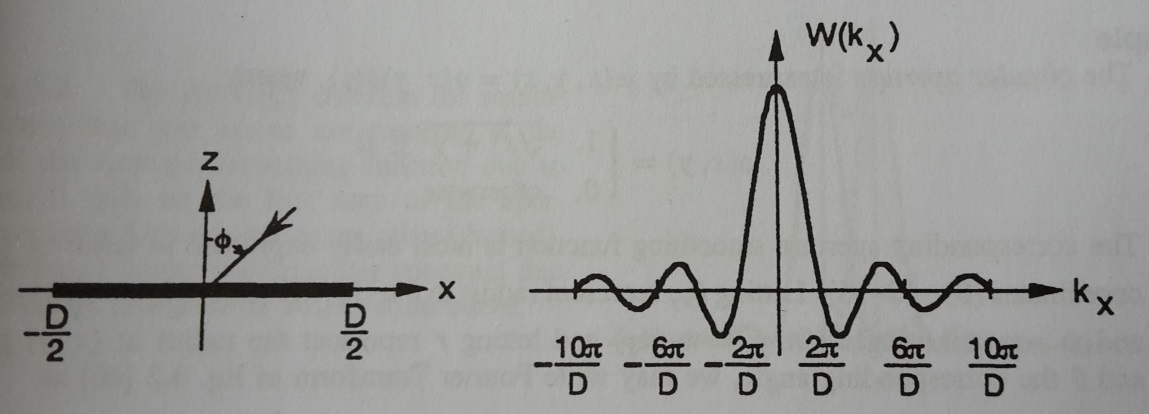
\includegraphics[width=\linewidth]{./images/background/linarray.jpg}
	\caption{Illustration of a linear array and its aperture smoothing function (Johnson and Dudgeon 1993, p.115)}
	\label{fig:linarray}
\end{figure}
\noindent
The transducer aperture smoothing function has a shape similar to a sinc function, with a mainlobe at $k_x = 0$ and sidelobes decreasing in amplitude as $k_x$ increases towards $\infty$ or decreases towards $-\infty$. Equation (\ref{eq:aperture_smoothing_linear}) also reveals that the longer the transducer is, the narrower the aperture smoothing function's mainlobe is. A narrow mainlobe is often a desired feature in beamforming, as it can increase the \textit{angular resolution} of the resulting image. There exists many definitions of \textit{resolution} in ultrasound imaging, which is why it may be confusing to compare results from different articles.

In this thesis, angular resolution is defined as the minimum distance between two reflectors for them to be resolved. This measure, often referred to as \textit{classical resolution} or \textit{resolvability}, is governed by the Rayleigh criterion. The Rayleigh criterion states that two incoherent plane waves propagating in different directions can be resolved if the distance between the mainlobe of their resulting aperture smoothing function replica is not smaller than half of the largest mainlobe width.

Notice however that the Rayleigh criterion only defines a theoretical maximum resolution and not an actual resolution measurement. Also, for this definition to make sense, one must define how mainlobe width is measured. Figure \ref{fig:linarray} shows that this width differs depending on the gain level. In this thesis, a mainlobe width is always measured at -3 dB gain from its peak. On the same note, two waves are considered \textit{resolved} only if the minima between their peaks is less or equal than the lowest peak gain minus 3 dB.

\subsection{Transducer arrays}
\label{sec:discrete_arrays}
A single transducer, even directional, can not give accurate spatial meaning to a recorded wavefield, since it only outputs an electrical signal $y_m(t)$ as a function of time.
The concept of \textit{beamforming} (Section \ref{sec:beamforming}) uses the combined output of multiple transducers to give spatial meaning to a recorded wavefield.
Such a combination of transducers is called a transducer \textit{array}. A transducer array can be of virtually any shape, for example circular, spherical or sparse.  The aperture function $w_m(\boldsymbol{x})$ of each transducer is defined by Equation (\ref{eq:aperture_linear}), but the array itself can also be considered to have an aperture shape $w_a(\boldsymbol{x})$, regardless of the shape of each transducer:
\begin{equation}
    w_a(\boldsymbol{x}) = \left \{ \begin{tabular}{cc}
        1, & x $\in \boldsymbol{X}_a$ \\
        0, & otherwise
    \end{tabular}\right.,
\label{eq:aperture_global}
\end{equation}
\noindent
where $\boldsymbol{X}_a$ is the set of positions $\boldsymbol{x}_m$ of the array elements.

Despite the theory presented being applicable to various array shapes, this thesis only focuses on discrete linear arrays of transducers able to both transmit and record signals, since it is the type of array simulated in this thesis and still one of the most widely used types of array in medical ultrasound.

Let us then assume a discrete linear array consisting of M infinitely small transducers uniformly distributed along the X axis, each separated by a distance D. Let us also consider that $x = 0$ is the center of the array. For simplicity, let us further assume that M is odd, so that the transducers can be numbered from $m = -(M-1)/2$ to $m = (M-1)/2$ and their position can be expressed simply as $x = m D$.
The array aperture function is then:
\begin{equation}
    w_a(\boldsymbol{x}) = \left \{ \begin{tabular}{cc}
        1, & x = m D, ~ y = 0, ~ z = 0 \\
        0, & otherwise
    \end{tabular}\right..
\label{eq:array_aperture}
\end{equation}
\noindent
The array aperture smoothing function, defined as the Fourier Transform of Equation (\ref{eq:array_aperture}), is:
\begin{align}
    W_a(\boldsymbol{k}) &= \int_{-\infty}^{\infty} w(\boldsymbol{x}) e^{j \boldsymbol{k} \cdot \boldsymbol{x}} d\boldsymbol{x} = \sum_{m=-(M-1)/2}^{(M-1)/2} e^{j k_x D m} \nonumber \\
    &= e^{-j k_x D (M-1)/2} k\sum_{m=0}^{M-1} e^{j k_x D m} \nonumber \\
    &= e^{-j k_x D M/2} e^{j k_x D/2} \frac{1 - e^{j k_x D M}}{1 - e^{j k_x D}} \nonumber \\
    &= \frac{2j}{2j} \frac{e^{-j k_x D M/2} - e^{j k_x D M/2}}{e^{-j k_x D/2} - e^{j k_x D/2}} \nonumber \\
    &= \frac{\sin(k_x D M/2)}{\sin(k_x D/2)},
\label{eq:array_aperture_smoothing}
\end{align}
\noindent
where the lemma $\sum_{n=0}^{N-1} r^n = \frac{1 - r^N}{1 - r}$ has been used.
\par
Equation (\ref{eq:array_aperture_smoothing}) reveals that the array smoothing function, unlike that of a single transducer (Equation (\ref{eq:aperture_smoothing_linear})), is periodic. This function is maximized for $k_x = n 2\pi/D, n \in \mathbb{Z}$, only one of which is the mainlobe ($k_x = 0$). The other maximas are called \textit{grating lobes}. This can result in \textit{spatial aliasing}, as signals propagating from different directions become indistinguishable.
However the array elements' own aperture geometry influence the array's total aperture $w_t(\boldsymbol{x})$.
The array aperture smoothing function of a discrete linear array can be defined as the product of a single element aperture smoothing function $W_m(\boldsymbol{k})$ and the one of the same array with infinitely small elements $W_a(\boldsymbol{k})$ (\cite{knut_landmark}):
\begin{equation}
    W_t(\boldsymbol{k}) \equiv W_m(\boldsymbol{k}) \cdot W_a(\boldsymbol{k}).
\end{equation}
\noindent
Figure \ref{fig:total_aperture} illustrates the effect of a transducer's aperture smoothing function applied to the one of the array. $W_m(\boldsymbol{k})$ is a non-periodic function, so the resulting effect is an attenuation of the array aperture smoothing function in all directions $\boldsymbol{k}$ with $k_x \neq 0$. One positive outcome of this attenuation is that the resulting function $W_t(\boldsymbol{k})$ has attenuated side lobes and grating lobes and is therefore less prone to signal propagation confusion.


\begin{figure}[ht]
    \centering
    \begin{subfigure}[b]{0.48\linewidth}
        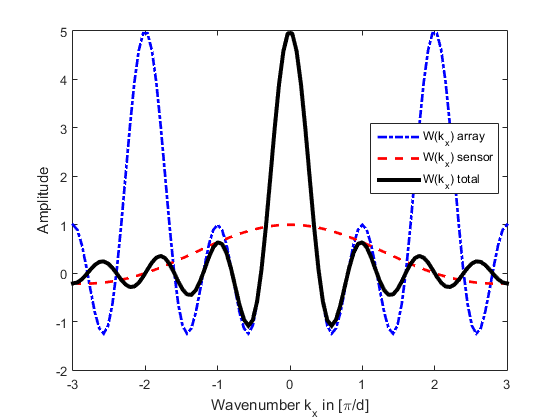
\includegraphics[width=\linewidth]{./images/background/bg_grating1.png}
        \caption{$W(k_x)$ amplitude}
    \end{subfigure}
    \quad
    \begin{subfigure}[b]{0.48\linewidth}
        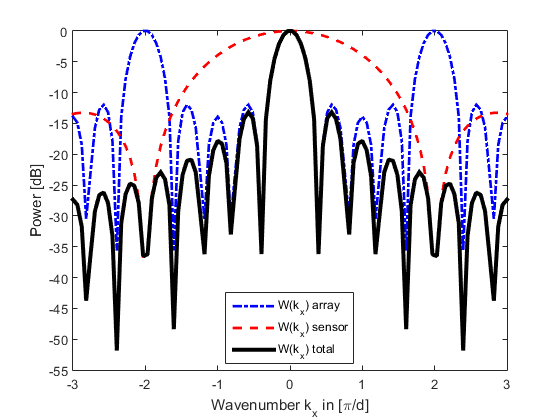
\includegraphics[width=\linewidth]{./images/background/bg_grating2.png}
        \caption{$W(k_x)$ power}
    \end{subfigure}
	\caption{Aperture smoothing function of discrete linear array of M=5 transducers}
	\label{fig:total_aperture}
\end{figure}


\section{Conventional beamforming}
\label{sec:beamforming}
Beamforming is a signal processing technique using multiple transducers to restrain the directionality of signals transmission or reception (\cite{DAS}). In the case of near-field beamforming (Section \ref{sec:nearfield_farfield}), this technique also restrains the range of focus. Medical ultrasound imaging is an example of a near-field scenario. And, since it uses active systems (Section \ref{sec:medical_imaging}), the beamforming can be done both on transmission and reception. This is often referred as \textit{two-way beamforming}, while \textit{one-way beamforming} designates beamforming on reception only. Although based on the same theory, beamforming on transmission and reception have two different goals:
\begin{itemize}
    \item Transmission: Produce signals such that they become all in phase at the focus point and result in a maximized energy radiation towards it.
    \item Reception: Align the recorded signals such that any potential signal coming from the focus point adds up coherently and maximizes its signal-to-noise ratio (SNR) when all recorded waveforms are summed together. The same approach can be applied to different focus points on the same signal measurements, which is why it is often referred to as \textit{dynamic focusing}.
\end{itemize}
\noindent
In this thesis, all beamformers use two-way beamforming and create beamformed images by sequentially transmitting narrow beams in a number of directions and, for each transmitted beam, dynamically delaying the received signals from all channels.

\subsection{Beamforming on transmission}
\label{sec:beamforming_transmission}
Whenever multiple waves are present in a wavefield, their superposition may result in interference.
As an example, let us imagine two monochromatic plane waves $s_1(\boldsymbol{x}, t)$ and $s_2(\boldsymbol{x}, t)$ of same frequency $\omega$ and amplitude $A$ being transmitted by two different emitters $t_1$ and $t_2$. The equation of such waves can be extracted from Equation (\ref{eq:mono_plane_wave}):
\begin{equation}
    s_i(x, t) = A ~ e^{j (\omega t - \boldsymbol{k}_i \cdot \boldsymbol{x} + \Phi_i)}, ~ i = [1, 2],
\end{equation}
\noindent
where $\Phi_i$ is the phase value of $s_i$ at position $\boldsymbol{x} = (0, 0, 0)$.
Let us have a receiver $r$ exposed to those waves. Its wavefield measurement $y_r(\boldsymbol{x}_r, t)$ is then, according to the superposition principle, equal to the sum of the two waves at that location and time:
\begin{align}
    y_r(\boldsymbol{x}_r, t) &= s_1(\boldsymbol{x}_r, t) + s_2(\boldsymbol{x}_r, t) \nonumber \\
    &= A ~ e^{j \omega t} (e^{-j (\boldsymbol{k}_1 \cdot \boldsymbol{x}_r - \Phi_1)} + e^{-j (\boldsymbol{k}_2 \cdot \boldsymbol{x}_r - \Phi_2)}),
\end{align}
\noindent
where $e^{-j (\boldsymbol{k}_1 \cdot \boldsymbol{x}_r - \Phi_1)} + e^{-j (\boldsymbol{k}_2 \cdot \boldsymbol{x}_r - \Phi_2)}$ is a periodic function with values in the [-2, 2] range, which means that, depending on the receiver's position $\boldsymbol{x}_r$, it can be exposed to energy amplitudes ranging from 0 to 2A. The waves interference is often referred to as \textit{constructive interference} when the recorded energy amplitude is higher than A, respectively \textit{destructive interference} when lower amplitude than A.

The example above shows that the effects of constructive interference can be used to achieve higher SNR than when transmitting a single signal.
Beamforming on transmission uses this physical property to aim towards a spatial point $\boldsymbol{x}_t$ and ensure constructive interference of its transmitted signals in that point.

Given an array of M transducers, each sending a signal $s_m(t) = s(t - \Delta_m)$, the delays $\Delta_m$ can be made such that constructive interference occurs at the focus point $\boldsymbol{x}_t$. The set of those time-based delays $\boldsymbol{e} = [\Delta_0, \Delta_1, ..., \Delta_{M-1}]^T$ can be seen as a beamforming focus vector, since it defines at which positions $\boldsymbol{x}$ constructive, and respectively destructive, interference occurs.


\subsection{Beamforming on reception}
\label{sec:beamforming_reception}
Given an array of M transducers and a set $Y(t) = [y_1(t), y_2(t), ..., y_M(t)]^T$, where $y_m(t)$ is the data recorded by transducer $m$.

Beamforming on reception can be done in a similar way as beamforming on transmission by creating a set of time-delays $\boldsymbol{e} = [\Delta_1, ..., \Delta_M]^T$ and applying the time-delays to the recorded data. Given any receive focus point $\boldsymbol{x}_r$, the time-delays set $\boldsymbol{e}_r$ is built such that any potential signal coming from $\boldsymbol{x}_r$ gets aligned coherently in the recorded data $Y(t)$.
Let us define the set of time-delayed recorded data $Y_e(t) = [y_{1e}(t), y_{2e}(t), ..., y_{Me}(t)]^T$, where $y_{me}(t) = y_m(t - \Delta_m)$.

Assuming a signal $s(t)$ sent towards the array from a source at position $\boldsymbol{x}_r$, each transducer's recorded wavefield $y_m(t)$ can be defined as:
\begin{equation}
    y_m(t) = s(t - \Delta_{rm}) + n_m(t),
\end{equation}
\noindent
where $\Delta_{rm}$ is a time delay attribute dependent on the position of transducer $m$ relative to the position of the source and the signal propagation properties, and $n_m(t)$ random noise recorded by transducer $m$.
The beamformer can focus on the source position by applying time delays equal to $-\Delta_{rm}$. Given $\boldsymbol{e}_r = [-\Delta_{r1}, -\Delta_{r2}, ..., -\Delta_{rM}]$, the time-delayed vectors $y_{me}(t)$ are then:
\begin{align}
    y_{me}(t) &= y_m(t - \Delta_m) = y_m(t + \Delta_{rm}) \nonumber \\
    &= s(t) + n_m(t + \Delta_{rm}).
\end{align}

The signal $s(t)$ can then be added constructively and result in a signal power $M$ times higher than if recorded by a single transducer. If the noise $n_m(t)$ recorded by each transducer is assumed to be white noise, it can be considered to be statistically uncorrelated to $n_i(t),~i \neq m$. This means that the sum of time-delayed signals also results in a signal SNR $M$ times higher than that of a single transducer recording.

Signals coming from other sources are expected to result in lower SNR than the one coming from $\boldsymbol{x}_r$, although, as seen in Section \ref{sec:aperture_smoothing}, this can not always be guaranteed.
The terms \textit{constructive} and \textit{destructive interference} are usually connoted to physical interference, so they are not used in this thesis for beamforming on reception to avoid confusion.


\subsection{Delay-And-Sum (DAS) beamforming}
\label{sec:DAS}
DAS beamforming is one of the simplest beamforming algorithms, yet still widely used in medical ultrasound imaging. The DAS beamformer's output signal can be defined as:
\begin{equation}
    z(t) \equiv \sum_{m=0}^{M-1} w_m y_m(t - \Delta_m),
\label{equ:das}
\end{equation}
\noindent
where $y_m(t - \Delta_m)$ is the data recorded by transducer $m$ after time-delay (Section \ref{sec:beamforming_reception}) and $w_m$ is the amplitude weight applied that data. If no shading (Section \ref{sec:sensor_arrays}) is applied, then $w_m = 1 \forall m \in \{0, 1, ..., M-1\}$. 
With the set of time-delayed received signals $\boldsymbol{Y}_e(t) = [y_{1e}(t), ..., y_{Me}(t)]^T$ defined as in Section \ref{sec:beamforming_reception}, Equation (\ref{equ:das}) can be rewritten in the vectorial form as:
\begin{equation}
    z(t) = \boldsymbol{w}^H \boldsymbol{Y_e}(t),
\end{equation}
\noindent
where $\boldsymbol{w}$ is the vector of amplitude weight values $w_m$ applied to transducer $m$ and $\boldsymbol{w}^H$ its conjugate transpose.

By using dynamic focusing on reception, a different time-based focus vector $\boldsymbol{e_x}$ can be defined for each focus point $\boldsymbol{x}$ in the imaged sector. 
The DAS beamformer output power can then be defined as a function of f $\boldsymbol{e_x}$:
\begin{equation}
\begin{split}
    Z(\boldsymbol{e_x}) \equiv E[|z(t)|^2](\boldsymbol{e_x}) = E\{(\boldsymbol{w}^H \boldsymbol{Y_{ex}})(\boldsymbol{w}^H \boldsymbol{Y_{ex}})^H\} \\
    = \boldsymbol{w}^H E\{\boldsymbol{Y_{ex}} \boldsymbol{Y_{ex}^H} \} \boldsymbol{w} = \boldsymbol{w}^H \boldsymbol{R_e} \boldsymbol{w},
\end{split}
\label{eq:das_power}
\end{equation}
\noindent
where $E[]$ is the expected value function and $\boldsymbol{R_e}$ is the \textit{spatial correlation matrix}, or \textit{covariance matrix}, of $\boldsymbol{Y_{ex}}$. Section \ref{sec:covariance_estimation} explains how this matrix can be estimated.

\subsection{Beamforming with narrowband signals}
\label{sec:beamforming_frequency}
Considering a monochromatic signal $s(t) = e^{j \omega t}$, a time-shift of $\Delta_m$ corresponds to a phase-shift of $e^{-j \omega \Delta_m}$:
\begin{equation}
    s(t - \Delta_m) = e^{j \omega (t - \Delta_m)} = e^{j \omega t} e^{-j \omega \Delta_m}.
\end{equation}
\noindent
Steering the transducers array can then easily be done by multiplying the set of received signals $Y_m(\omega)$ with a set of phase delays $e^{-i \omega \Delta_m}$. This set of phase-delays define the beamformer's phase-based \textit{steering vector} \textbf{a}.
Unlike the time-based focus vector \textbf{e} (Section \ref{sec:beamforming_transmission}), the phase-based one is only properly defined for a single frequency $\omega$. In fact, for any frequency $\omega_2 \neq \omega$, the phase shift $e^{-i \omega \Delta_m}$ differs of that of the $e^{-i \omega_2 \Delta_m}$ phase required for constructive signals superposition at the chosen focus point.

Although only valid for monochromatic waveforms, the phase-based steering approach is often used in narrowband applications, for which most of the energy radiated or recorded is within a small frequency bandwidth relative to the center frequency. In such scenarios, the phase shift difference $e^{-i (\omega_2 - \omega) \Delta_m}$ can be considered negligible.
In broadband applications, such as ultrasound medical imaging, the phase shift difference can only be considered negligible for small shifts, meaning for steering angles close to perpendicular to the array. For larger steering angles, the time-based dynamic focusing approach (Section \ref{sec:beamforming_reception}) can be used to fall back to reasonable phase shifts (\cite{Jensen_multibeam}). This technique is used throughout this thesis and all the theory presented from this point on is focusing on monochromatic waveforms.


\subsection{Near-field and far-field beamforming}
\label{sec:nearfield_farfield}
As mentioned in Section \ref{sec:prop_waves}, waves do not propagate along a single direction, but in all directions such that the set of coordinates with the same wave phase looks like a sphere, as illustrated in Figure \ref{fig:farfield}. Due to this type of propagation, sensors at different locations can experience a different wave propagation direction. This seems logical since the source of the propagating wave is potentially located at different relative orientations to each sensor. It is this difference in relative propagation direction that allows the possibility to focus a sensor array to a specific point in space.

However, if a wave's direction of propagation is approximately equal for all sensors, the perceived waveform resembles more the one of a plane wave, as illustrated in Figure \ref{fig:farfield}. This scenario can occur if the source of the propagating wave is located far from the array and plane wave approximation (Section \ref{sec:prop_waves}) can be applied. In that case, beamforming can resolve the source orientation but not its distance to the array.

Sources located close enough to the array to extract their distances to it are said to be in the array's \textit{near field}, whereas sources beyond that are said to be in its \textit{far field}. In most cases, the focus of interest is either in the near field or in the far field and different beamforming algorithms are usually used in either case. Therefore the terms \textit{nearfield beamforming} and \textit{farfield beamforming} are often used to differentiate the two scenarios.

The crossover distance $d_c$ between near field and far field is not a hard-defined one. It is based on deciding at which distance to the array the different wave propagation directions perceived by each sensor can be approximated to equal directions with a negligible phase error. The definition of negligible can vary a lot depending on the beamforming application and expected outcome.

An intuitive example of the crossover distance for linear arrays can be found in \cite{wright_compendium}. This example's crossover distance is $d_c = A^2 / \lambda$, where $A$ is the length of the linear array and $\lambda$ is the maximum signal wavelength present in the recorded wavefield.
In conventional ultrasound imaging, the array's length is typically in the order of centimeters, whereas the signals transmitted are in the order of $MHz$. Given the crossover distance $d_c = A^2 / \lambda$, most of the medical ultrasound imaging applications occur in the array's near field.

\begin{figure}[ht]
    \centering
    \begin{subfigure}[b]{0.48\linewidth}
        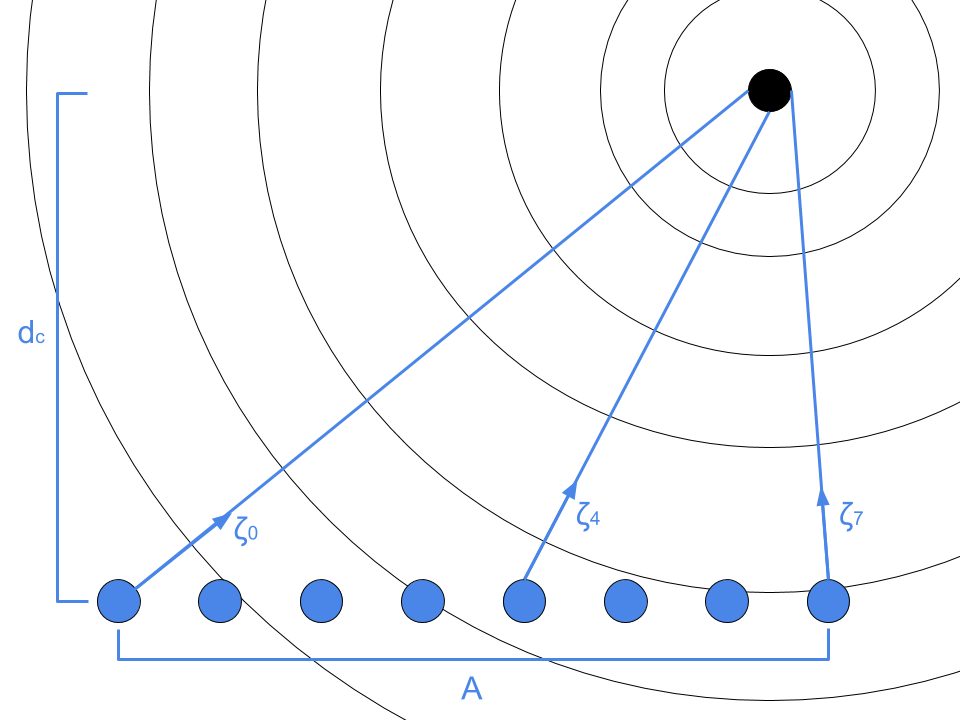
\includegraphics[width=\linewidth]{./images/background/nearfield.png}
        \caption{Nearfield}
    \end{subfigure}
    \quad
    \begin{subfigure}[b]{0.48\linewidth}
        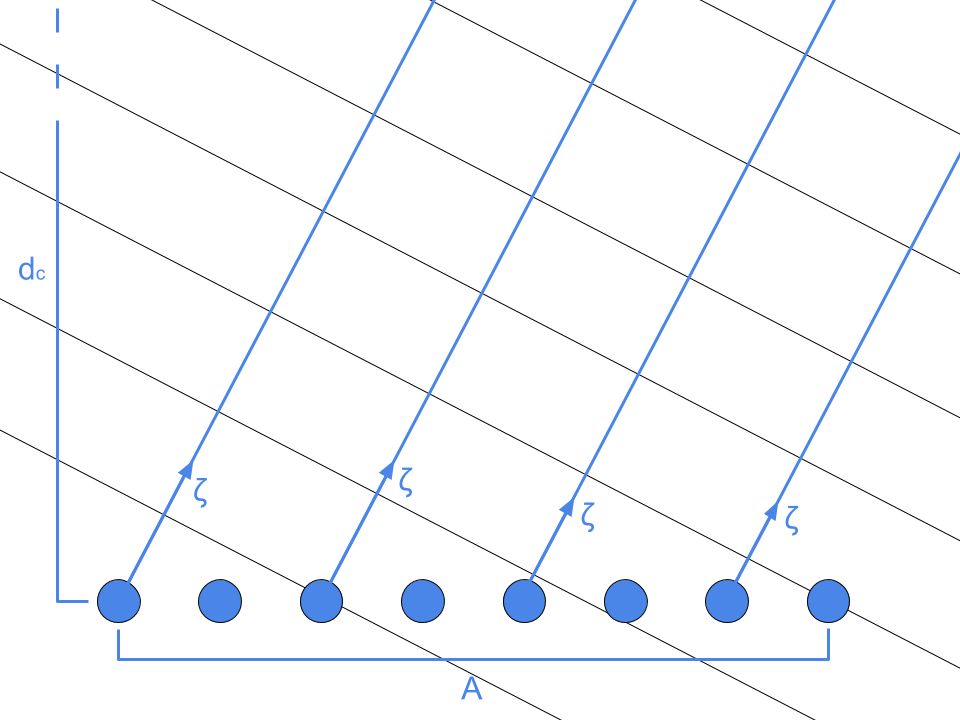
\includegraphics[width=\linewidth]{./images/background/farfield.png}
        \caption{Farfield}
    \end{subfigure}
	\caption{Illustrations of nearfield and farfield beamforming. The black lines and curves represent planes of constant phase.}
	\label{fig:farfield}
\end{figure}


\subsection{Beampattern and steered response}
\label{sec:beampattern} 
An array's aperture smoothing function, or array pattern, $W(\boldsymbol{k})$ defines its response to a monochromatic plane wave.
For a discrete array of M transducers, its aperture function $w(\boldsymbol{x})$ is defined by Equation (\ref{eq:aperture_global}) and its array pattern $W(\boldsymbol{k})$ from Equation (\ref{eq:array_aperture_smoothing}) as:
\begin{equation}
    W(\boldsymbol{k}) = \int_{\mathbb{R}^3} w(\boldsymbol{x}) e^{j \boldsymbol{k} \cdot \boldsymbol{x}} d\boldsymbol{x} = \sum_{m=0}^{M-1} w_m e^{j \boldsymbol{k} \cdot \boldsymbol{x}_m}, 
\label{eq:bp_aas}
\end{equation}
\noindent
where $\boldsymbol{x}_m$ is the position of transducer $m$.

Assuming a monochromatic plane wave $s(\boldsymbol{x},t)$ of temporal frequency $\omega^0$ and slowness vector $\boldsymbol{\alpha}^0$ and no other signal or noise, the resulting wavefield $f(\boldsymbol{x},t)$ is then:
\begin{equation}
    f(\boldsymbol{x},t) =  s(\boldsymbol{x},t) = s(t - \boldsymbol{\alpha}^0 \cdot \boldsymbol{x}) = e^{j \omega^0 (t - \boldsymbol{\alpha}^0 \cdot \boldsymbol{x})},
\label{eq:bp_mono}
\end{equation}
\noindent
where $s(t - \boldsymbol{\alpha}^0 \cdot \boldsymbol{x})$ comes from Equation (\ref{eq:mono_plane_wave}).
The DAS beamformer output defined in Equation (\ref{equ:das}) is then:
\begin{equation}
    z(t) = \sum_{m=0}^{M-1} w_m s(t - \boldsymbol{\alpha}^0 \cdot \boldsymbol{x}_m - \Delta_m),
\label{eq:bp_das}
\end{equation}
\noindent
where $\Delta_m$ is the time delay applied to the signal recorded by transducer $m$.
As explained in Section \ref{sec:prop_waves}, for a monochromatic signal, this time delay can also be expressed as a phase delay $\phi = \omega^0 \boldsymbol{\zeta}_m \boldsymbol{x}_m / c$, where $\boldsymbol{\zeta}_m$ is the direction of focus of transducer $m$ and $c$ the signal's propagation speed.
Furthermore, if that signal is considered to be a plane wave, all transducer have the same direction of focus $\boldsymbol{\zeta}$.
To simplify the comparison between the array's focus and the recorded wavefield properties, we say that the array is looking for signals propagating with slowness vector $\boldsymbol{\alpha} = -\boldsymbol{\zeta}/c$. The minus sign represents the fact that $\boldsymbol{\zeta}$ is the orientation of the array as a vector originating from it and directed outwards, whereas the signals it is looking for are expected to originate away from the array and propagate towards it.
This definition allows for a more intuitive expression of Equation (\ref{eq:bp_das}):
\begin{equation}
    z(t) = \sum_{m=0}^{M-1} w_m s(t + (\boldsymbol{\alpha} - \boldsymbol{\alpha}^0) \cdot \boldsymbol{x}_m).
\label{eq:bp_das_alpha}
\end{equation}

Equation (\ref{eq:bp_das_alpha}) shows that a signal originating at the array's focus point is then added coherently by the DAS beamformer.
It also reveals that the DAS output can be expressed as a function of $W(\cdot)$. Indeed, combining Equations (\ref{eq:bp_aas}), (\ref{eq:bp_mono}) and (\ref{eq:bp_das_alpha}) yields the following equation:
\begin{align}
    z(t) &= \sum_{m=0}^{M-1} w_m e^{j \omega^0 (t + (\boldsymbol{\alpha} - \boldsymbol{\alpha}^0) \cdot \boldsymbol{x})} \nonumber \\
    &= e^{j \omega^0 t} \sum_{m=0}^{M-1} w_m e^{j (\omega^0 \boldsymbol{\alpha} - \boldsymbol{k}^0) \cdot \boldsymbol{x}_m} \nonumber \\
    &= e^{j \omega^0 t} W(\omega^0 \alpha - \boldsymbol{k}^0),
\end{align}
\noindent
where $\boldsymbol{k}^0 = \omega^0 \boldsymbol{\alpha}^0$ is the wavenumber vector of $s(t)$.

This equation shows that, under the monochromatic plane wave assumption, the DAS beamformer can be seen as a linear and time-invariant system.
Indeed, considering a linear and time-invariant system, its output equals the recorded wavefield $f(\boldsymbol{x},t) = s(\boldsymbol{x}, t)$ convolved with the system's impulse response $h(\boldsymbol{x}, t)$ (\cite{Dudgeon_book}).
In the frequency domain, this convolution becomes a multiplication:
\begin{equation}
    z(\boldsymbol{x}, t) = s(\boldsymbol{x}, t) * h(\boldsymbol{x}, t) ~~ \overset{F}{\Longrightarrow} ~~  Z(\boldsymbol{k}^0, \omega^0) = S(\boldsymbol{k}^0, \omega^0) H(\boldsymbol{k}^0, \omega^0),
\end{equation}
where $*$ is the convolution operator and $H(\boldsymbol{k}^0, \omega^0)$ is the frequency domain expression of the system's impulse response. The notation $\boldsymbol{k}^0$ and $\omega^0$ is kept in order to avoid confusion with the array's targeted slowness vector $\boldsymbol{\alpha} = \boldsymbol{k} / \omega$.
With $s(\boldsymbol{x},t)$ as defined by Equation (\ref{eq:bp_mono}), its Fourier transform is $S(\boldsymbol{k}^0, \omega^0) = e^{j \omega^0 t}$.
The system's space-time filter $h(\boldsymbol{x}, t)$ is therefore built such that $H(\boldsymbol{k}^0, \omega^0) = W(\omega^0 \boldsymbol{\alpha} - \boldsymbol{k}^0)$. This space-time filter is often referred to as the \textit{wavenumber-frequency response} of a linear and time-invariant system.

The expression of the wavenumber-frequency response $W(\omega^0 \boldsymbol{\alpha} - \boldsymbol{k}^0)$ shows that its input $\omega^0 \boldsymbol{\alpha} - \boldsymbol{k}^0$ is a combination of both the wavefield's propagation parameters $\boldsymbol{k}^0$ and $\omega^0$ as well as the array's configuration $\boldsymbol{\alpha}$.
The analysis of the wavenumber-frequency response can then be interestingly partitioned into two different angles of observation.
One focused on the effects of different wavefield parameters with a fixed array configuration. This corresponds to $W(\omega^0 \boldsymbol{\alpha} - \boldsymbol{k}^0)$ with fixed $\boldsymbol{\alpha}$ and is known as the array's \textit{beampattern}.
The second approach is to analyze the effects of different array configurations given a fixed wavefield. This corresponds to $W(\omega^0 \boldsymbol{\alpha} - \boldsymbol{k}^0)$ with fixed  $\omega^0$ and $\boldsymbol{k}^0$ and is known as the array's \textit{steered response}.


\subsection{Parallel-receive beamforming}
\label{sec:prb}
When performing ultrasound imaging of moving structures, such as a moving heart, relatively high image acquisition rates are often required.
One common way to increasing frame rate while maintaining high resolution is using a higher beam density on reception (Section \ref{sec:beamforming_reception}) than on transmission (Section \ref{sec:beamforming_transmission}). 
This approach is often referred to as \textit{parallel-receive beamforming} (PRB, \cite{prb_approaches}) or \textit{multiple-line acquisition} (MLA), in opposition to the traditional \textit{single-line acquisition} (SLA) approach.

The concept is to use the imperfect beamforming on transmission by creating multiple receive beams per transmit beam in order to extract information available in several directions. The beamforming on transmission is said here to be imperfect because energy is not only radiated towards the transmit beam's focus point, but also in other directions. A beamformer can then potentially use this phenomenon to detect signals backscatterered by scatterer points in directions where energy is sent.

However, the misalignment between transmit and receive beams causes several geometric distortions in their corresponding two-way beampattern.
Those distortions are separated in \cite{prb_approaches} into three categories: Beam wrapping, beam skewing and energy loss.

Beam wrapping, also known as beam wander, is the effect that the two-way beam does not follow a straight line. When the transmit and receive beams are not aligned, the transmit beam pulls the two-way beam towards its center.
This phenomenon is illustrated in Figure \ref{fig:prb}, where the direction-of-arrival (DOA) of two-way beam is visibly in between those of the transmit and receive beams.

For linear arrays, both the transmission beampattern and the reception one are symmetric functions. Yet, when they are not aligned, the two-way beampattern can become non-symmetric. This effect is known as beam skewing. In Figure \ref{fig:prb}, the skewing is most apparent around the local minimas of the two-way beampattern, especially by comparing the local minimas at ~$-2.2^\circ$ and $3.2^\circ$ DOA.

Energy loss is visible in Figure \ref{fig:prb} with the two-way beampattern having a general lower gain than that of the transmission and reception ones.
Misalignment between transmission and reception beams causes then loss in signal-to-noise ratio (SNR). Furthermore, the scale of SNR drop is dependent on the level of misalignment.

\begin{figure}[ht]
    \centering
    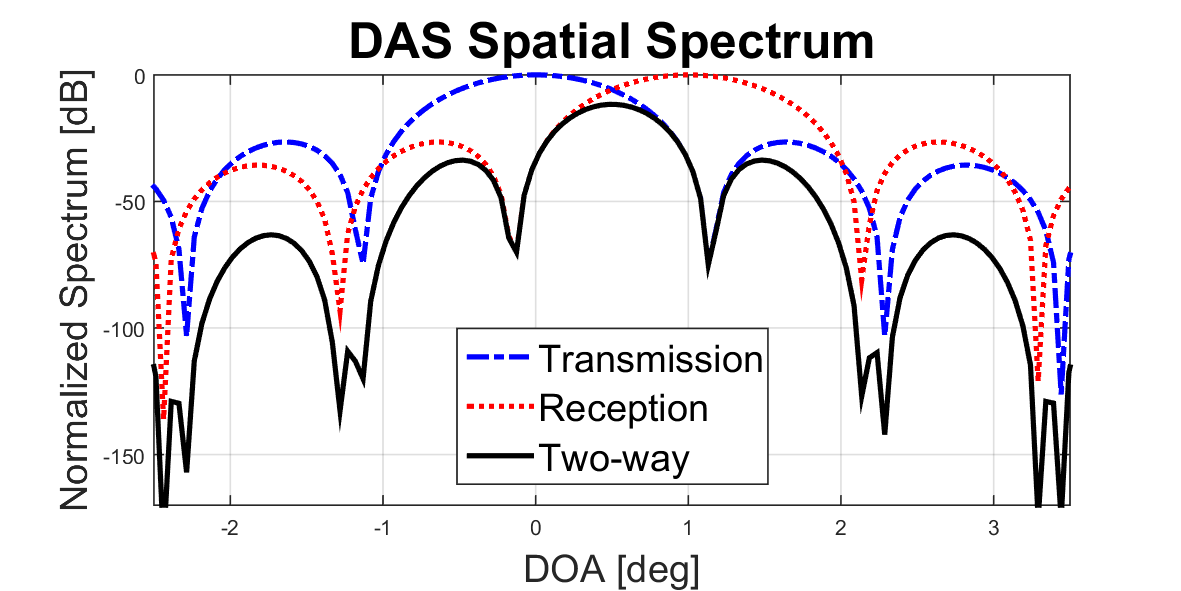
\includegraphics[width=\linewidth]{./images/background/prb.png}
	\caption{Example of DAS transmission, reception and two-way beampatterns with misalignment of transmit and receive beams}
	\label{fig:prb}
\end{figure}

An example of PRB approach is displayed in Figure \ref{fig:prb_3beams}. Three two-way beams are created from a single transmit beam, which means that image acquisition time can be reduced in this case by a factor of three without resolution loss. However, the two-way beams that are not aligned with the transmit beam display lower maximal gain than the one that is aligned.
Their maxima, at -0.5 and $0.5^\circ$ DOA, is also shifted towards that of the transmit beam compared that of their relative receive beams, at -1 and $1^\circ$ DOA.

Several approaches to reducing artifacts caused by PRB exist. Some of them, known as synthetic transmit beams, dynamic steering or the Wright approach, are explained and compared by \cite{prb_approaches}.

\begin{figure}[ht]
    \centering
    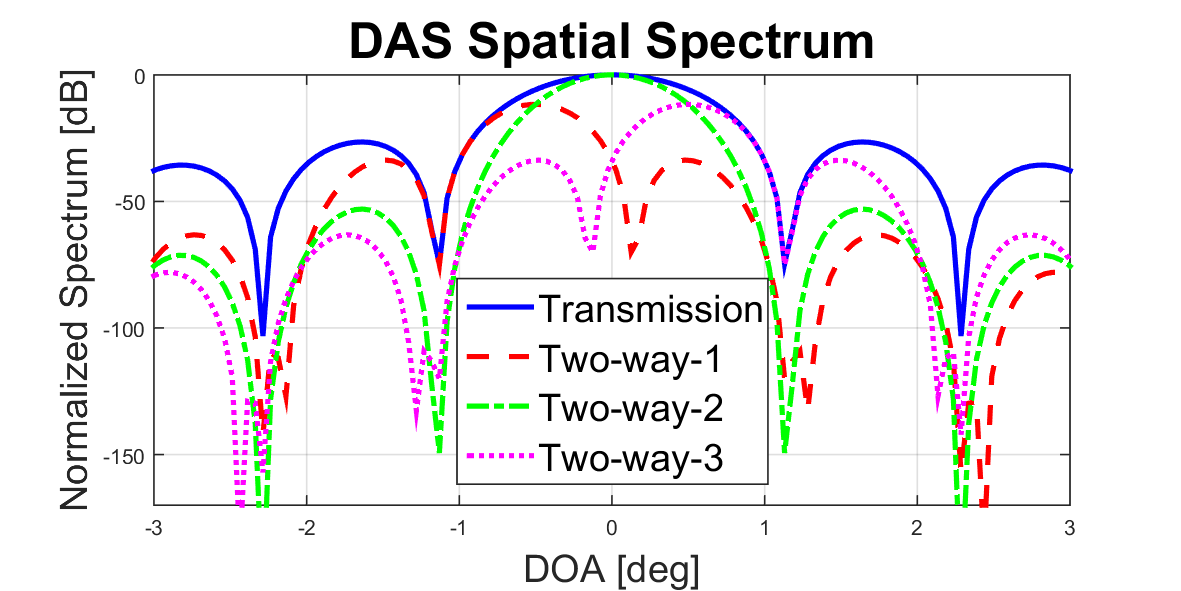
\includegraphics[width=\linewidth]{./images/background/prb_3beams.png}
	\caption{Example of PRB approach, with a single transmit beam centered at $0^\circ$ and 3 receive beams at -1, 0 and $1^\circ$. The resulting two-way beampatterns are displayed along with the transmit beam.}
	\label{fig:prb_3beams}
\end{figure}


\subsection{Covariance matrix estimation}
\label{sec:covariance_estimation}
The covariance matrix of the set of time-delayed recorded signals $\boldsymbol{Y_e}(t)$ is defined $\boldsymbol{R_e}(t) = E[\boldsymbol{Y_e}(t) \boldsymbol{Y_e}^H(t)]$.
Assuming the transducer array to record only monochromatic waves in the far-field (Section \ref{sec:nearfield_farfield}), $\boldsymbol{Y_e}(t)$ can be considered as a \textit{stationary process} in time, which means $\boldsymbol{R_e}$ is only dependent on the focus vector $\boldsymbol{e}$. Considering that all backscatterers in the imaged medium are uncorrelated and $\boldsymbol{Y_e}$ is a stationary process, $\boldsymbol{R_e}$ is a Toeplitz matrix (\cite{van_trees}). A Toeplitz matrix is a matrix whose descending left-to-right diagonals are constants. It notably has the property of being \textit{persymmetric}:
\begin{equation}
    \boldsymbol{R} = \boldsymbol{JR^TJ}, \quad J = \begin{bmatrix}
    0 & 0 & ... & 0 & 1 \\
    0 & 0 & ... & 1 & 0 \\
    : & : & ... & : & : \\
    0 & 1 & ... & 0 & 0 \\
    1 & 0 & ... & 0 & 0
    \end{bmatrix},
\label{eq:persymmetric}
\end{equation}
\noindent
where $\boldsymbol{J}$ is a MxM exchange matrix. This property is notably used by the \textit{forward-backward} approach (Section \ref{sec:fb_averaging}).
\noindent
This matrix is used in Equation (\ref{eq:das_power}) for obtaining the DAS beamformer power output $Z(\boldsymbol{e})$. However, this matrix is unknown and an estimate of it, $\boldsymbol{\tilde{R}(e)}$, needs to be built.

In medical ultrasound imaging, the recorded signals are often broadband and in the array's near field. The assumption that $\boldsymbol{Y}$ is a stationary process is therefore often not true.
However, instead of building a global covariance matrix estimate $\boldsymbol{\tilde{R}}$ for the whole beamformed image, a different covariance matrix estimate $\boldsymbol{\tilde{R}}_{\theta,n}$ can be built for each image sample $Z_{\theta, n}$, i.e each sample range index $n$ and angle index $\theta$.
Note that a range index $n$ can consist of a multiple temporal samples $t$ of the recorded wavefield $\boldsymbol{Y}(t)$ if time averaging (Section \ref{sec:time_averaging}) is used.
The discrete covariance matrix estimate $\boldsymbol{\tilde{R}}_{\theta,n}$ can be expressed as follow:
\begin{equation}
    \tilde{\boldsymbol{R}}_{\theta,n} = \frac{1}{2T+1} \sum_{t=-T}^{T} \boldsymbol{Y_e}[n - t] \boldsymbol{Y_e}^H[n - t],
\label{eq:cov_matrix}
\end{equation}
\noindent
where $2T + 1$ is the number of temporal samples per radial range and $\boldsymbol{Y_e}$ is the set of recorded wavefield time-shifted by vector $\boldsymbol{e}$. The time-delay focus vector $\boldsymbol{e}$ can be defined as a function of $n$ and $\theta$.
The local estimates of $\boldsymbol{R_e}$ should then technically be defined as $\boldsymbol{\tilde{R}}_{\boldsymbol{e}(\theta,n)}$.
We have chosen to simplify the notation to $\tilde{\boldsymbol{R}}_{\theta,n}$.

Yet, even for local estimates of $\boldsymbol{R_e}$, $\boldsymbol{Y_e}$ is not always stationary. In medical ultrasound imaging, it is often the case that the transducer array is sending short pulses and only recording a few temporal samples $t$ per radial range $n$. This means that the pulse reflected by a target out of the array's focus might not be recorded by all transducers for the same sample range $n$. However, the stationary assumption holds for targets close to the array's focus point, since the recorded data is aligned such that their reflected signal adds up coherently.
    
\section{Adaptive beamforming}
\label{sec:adaptive_beamforming}
Adaptive beamformers, unlike conventional ones, can adapt their aperture weights depending on the recorded wavefield. This adaptive nature allows to build steered responses (Section \ref{sec:beampattern}) with narrower mainlobe by allowing large side-lobes in directions in which there is no/little received energy, thus enduring no/limited energy leakage. This often results in improved image resolution and noise suppression, but at the cost of higher computational complexity.

\subsection{Minimum Variance (MV) beamforming}
\label{sec:MV}
The MV beamformer, also known as Capon beamformer (\cite{Capon}), uses what may be the most straightforward approach to adaptive beamforming. The approach is to minimize the beamformer's global output power (Equation \ref{eq:das_power}) while maintaining a unit gain in its steering direction. Note that this limitation is the reason this beamformer is classed as a \textit{distortionless} beamformer, which is why it is also often referred to as the Minimum Variance Distortionless Response (MVDR) beamformer. In mathematical terms, this comes to solving the following constrained optimization problem:
\begin{equation}
    \min_{\boldsymbol{w}} \boldsymbol{w}^H \boldsymbol{R_e} \boldsymbol{w}, \quad subject ~ to \quad \boldsymbol{w}^H \boldsymbol{1} = 1,
\label{eq:mv_problem}
\end{equation}
\noindent
where $\boldsymbol{w} = [w_1, ..., w_M]^T$ is the set of weights applied to the array transducers $[1,...,M]$, the vector $\boldsymbol{1}$ is a vector of length $M$ whose elements are all equal to 1, $\boldsymbol{e}$ is the beamformer focus vector on reception, as defined in Section \ref{sec:beamforming_reception}, and $\boldsymbol{R_e} = E[\boldsymbol{Y_e} \boldsymbol{Y_e}^H]$ is the covariance matrix of $\boldsymbol{Y_e}(t)$ and $\boldsymbol{Y_e}(t) = [y_{1e}(t), ..., y_{Me}]^T$ is the set of the signals recorded by the array transducers and time-delayed by $\boldsymbol{e}$.

As mentioned in Section \ref{sec:covariance_estimation}, $\boldsymbol{R_e}$ is unknown and needs to be estimated.
Local covariance matrix estimates $\boldsymbol{\tilde{R}}_{\theta,n}$ can be built from Equation (\ref{eq:cov_matrix}) for each angle index $\theta$ and sample range $n$ of the beamformed image $Z(\theta,n)$.
If the array is steered using the phase-based approach presented in Section \ref{sec:beamforming_frequency}, Equation (\ref{eq:mv_problem}) can be written as:
\begin{equation}
    \min_{\boldsymbol{w}} \boldsymbol{w}^H \boldsymbol{\tilde{R}}_{\theta,n} \boldsymbol{w}, \quad subject ~ to \quad \boldsymbol{w}^H \boldsymbol{a} = 1,
\label{eq:mv_problem_fixed}
\end{equation}
\noindent
where $\boldsymbol{a}$ is the array's phase-based steering vector.
The solution to this minimization problem is:
\begin{equation}
    \boldsymbol{w} = \frac{\boldsymbol{\tilde{R}}_{\theta,n}^{-1} \boldsymbol{a}}{\boldsymbol{a}^H \boldsymbol{\tilde{R}}_{\theta,n}^{-1} \boldsymbol{a}}.
\label{eq:mv_weight}
\end{equation}

\noindent
The MV beamformer power output is therefore:
\begin{equation}
    Z(\boldsymbol{a}) = \boldsymbol{w}^H \boldsymbol{\tilde{R}}_{\theta,n} \boldsymbol{w} =
    \frac{1}{\boldsymbol{a}^H \boldsymbol{\tilde{R}}_{\theta,n}^{-1} \boldsymbol{a}}.
\label{eq:mv_power}
\end{equation}
\noindent
$\boldsymbol{\tilde{R}}_{\theta, n}$ is often computed from $2T+1 < M$ observations, where $2T+1$ is the number of temporal samples and $M$ the number of receiving transducers in the array.  As $rank(\boldsymbol{\tilde{R}}_{\theta, n}) \leq min(2T+1, M)$, the matrix is often rank-deficient, therefore not invertible (\cite{Vignon_Focused}). Furthermore, if not all observations are independent, $rank(\boldsymbol{\tilde{R}}_{\theta, n})$ becomes strictly less than T. Due to this condition, $\boldsymbol{\tilde{R}}_{\theta, n}$ is often pseudo-inverted rather than truly inverted. It must also often be \textit{diagonally loaded} (Section \ref{sec:diagonal_loading}) to ensure a robust (pseudo-)inversion.

The MV approach can result in a major increase in resolution, but not without cost.
Although narrow beams increase the image resolution, one fundamental drawback is that more beams are required to image the same angular range and avoid \textit{angular undersampling}. Angular undersampling occurs when the angle between two beams' mainlobes becomes so large that it results in angles for which signals are heavily attenuated or suppressed. Scatterer points can then appear weaker or completely disappear from the beamformed image if in between two beams. This signal attenuation effect is often referred to as \textit{scalloping loss}. This effect can be attenuated by forming wider beams and/or more beams.

As Equations (\ref{eq:mv_weight}) and (\ref{eq:mv_power}) might hint, one major drawback of the MV beamformer, in comparison to DAS, is its computational complexity.
$\boldsymbol{\tilde{R}_{\theta,n}}$ has to be created, inverted and then applied. The matrix inversion is a very time consuming operation (complexity $O(M^3)$, where $M$ is the number of receiving transducers).

\subsection{Diagonal loading}
\label{sec:diagonal_loading}
The MV beamformer is particularly sensitive to divergences between the array and medium assumed model and their true model. Such divergences can for example be inaccuracies in the speed of signals propagation in the medium, differences in the sensors sensitivity or the presence of faulty sensors.

\textit{Diagonal loading} is a technique used to increase robustness to such divergences in the model by adding a small value $\epsilon$ to the diagonal of the covariance matrix estimate:
\begin{equation}
    \boldsymbol{\hat{R}}_{\theta, n} = \boldsymbol{\tilde{R}}_{\theta, n} + \epsilon \boldsymbol{I},
\end{equation}
\noindent
where $\epsilon$ is typically chosen as a fragment of the trace of $\boldsymbol{\tilde{R}}_{\theta, n}$ (\cite{Synnevag_adaptive}):
\begin{equation}
    \epsilon = \delta tr\{\boldsymbol{\tilde{R}}_{\theta, n} \} / L,
\end{equation}
\noindent
where $\delta \geq 0$ is the \textit{diagonal loading factor}, typically taken as a user parameter, and $L$ is the size of the subarrays used for \textit{spatial smoothing} (Section \ref{sec:spatial_smoothing}).

This approach is conceptually similar to adding spatially white noise to the recorded signals and results in a wider mainlobe of the steered response (\cite{Synnevag_adaptive}). The value $\epsilon$ influences therefore directly the width of the steered response's mainlobe and is a trade-off between image resolution and beamformer robustness to errors in the model. Note that as $\epsilon$ increases, the covariance matrix estimate $\boldsymbol{\hat{R}}_{\theta, n}$ loses more of its adaptive nature and, if $L=M$, converges towards the one of the conventional DAS beamformer.

\subsection{Spatial smoothing}
\label{sec:spatial_smoothing}
Since medical imaging is a domain using mainly active systems (Section \ref{sec:ultrasound_imaging}), most of the recorded signals are echoes from the same transmitted signals and are therefore generally highly correlated, or \textit{coherent}. This coherency between the received signals can cause noticeable signal cancellation and result in lower SNR.
Figure \ref{fig:spatial_smoothing} illustrate this effect with two closely-separated scatterer points.

In order to correct this effect, the coherent signals have to be decorrelated. \textit{Spatial smoothing}, also known as \textit{spatial filtering} or \textit{subarray averaging}, is a method first introduced by \cite{Evans_spatial} to decorrelate the signal of interest from the noise-and-interference signals. The approach divides the receiver array of M elements into K smaller overlapping arrays of L elements, where $K = M - L + 1$ and $1 \leq L \leq M$. The covariance matrix estimate $\boldsymbol{\hat{R}}_{\theta, n}$ can then be built by averaging the covariance matrix estimates of all K subarrays:
\begin{equation}
    \boldsymbol{\hat{R}}_{\theta, n} = \frac{1}{K} \sum_{k=0}^{K-1} \boldsymbol{\hat{R}_k}(\theta, n),
\label{eq:mv_spatial}
\end{equation}
\noindent
where each subarray covariance matrix estimate $\boldsymbol{R_k}(\theta, n)$ is defined by Equation (\ref{eq:cov_matrix}). If no temporal averaging (Section \ref{sec:time_averaging}) is used, Equation (\ref{eq:mv_spatial}) can be expressed as:
\begin{equation}
    \boldsymbol{\hat{R}}_{\theta, n} = \frac{1}{K} \sum_{k=0}^{K-1} \boldsymbol{Y_k}[n] \boldsymbol{Y_k}^H[n],
\end{equation}
\noindent
where, for each subarray $k$, $\boldsymbol{Y_k}$ is the set of recorded wavefield time-delayed and/or phase-shifted to focus on angle index $\theta$ and range index $n$.

$L$ is often taken as a user parameter and its value chosen depending on the application. As $L$ converges towards $M$, the covariance matrix estimate converges to the original one and the beamformer converges to the original MV beamformer. On the other hand, as $L$ converges towards 1, each element gets considered as an array and the beamformer converges to the conventional DAS beamformer. The choice of $L$ is then a trade-off between image resolution and robustness to signal coherence.
\par
Figure \ref{fig:spatial_smoothing} illustrates the effects of spatial smoothing by comparing the steered response of 4 beamformers variants:
\begin{enumerate}
    \item Conventional DAS beamforming, no spatial smoothing
    \item MV beamforming without spatial smoothing, L = M
    \item MV beamforming with long subarray length, L = 3 M / 4
    \item MV beamforming with half subarray length, L = M / 2
\end{enumerate}

\noindent
An array of $M=100$ sensors is simulated and two coherent signals in random Gaussian noise are generated at -1 and 1 degrees direction-of-arrival (DOA) from the array center. In this scenario, the standard MV beamformer suffers extreme signal cancellation. As expected spatial smoothing succeeds in partially decorrelating the two signals and attenuating the signal cancellation.

\begin{figure}[ht]
    \centering
    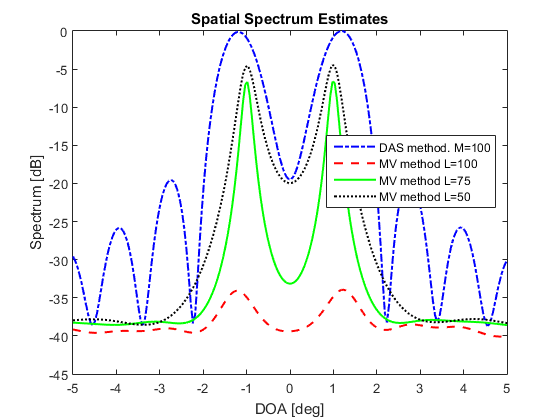
\includegraphics[width=\linewidth]{./images/background/spatial_averaging.png}
    \caption{Effects of spatial smoothing with coherent signals.}
    \label{fig:spatial_smoothing}
\end{figure}


\subsection{Time averaging}
\label{sec:time_averaging}
The MV beamformer has shown to be able to achieve higher resolvability of scatterer points than the conventional DAS. However, the spatial covariance matrix estimate used in the MV beamformer affects the patterns of homogeneous tissue. Homogeneous tissues are typically represented in beamformed images by \textit{speckle}, which consists of the transmitted signals scattered by a large number of small, densely distributed, scatterer points. In this thesis, speckle is generated by simulating a large number of small scatterer points uniformly distributed in the medium.
\cite{speckle} showed that the MV beamformer has a tendency to attenuate the homogeneity of the speckle and may give the impression of scatterer points existing in the homogeneous tissue.
Spatial averaging can enhance scatterer points resolution, but tend to result in lower average speckle magnitude. This effect can be beneficial for certain applications, as it tends to improve the SNR of isolated scatterer points, but can be undesirable in applications that use speckle in their image formation and/or analysis (e.g. skin tissue imaging).

Temporal averaging is a solution proposed by \cite{speckle} to reduce the effect of spatial averaging on speckle. Temporal averaging consists of using multiple samples per range for the spatial covariance matrix estimation. The idea is to allow a better capture of the speckle statistics by using multiple temporal samples, to the expense of reduced spatial resolution in the range dimension. Equation (\ref{eq:mv_temp}) reflects the addition of temporal averaging on Equation (\ref{eq:cov_matrix}):
\begin{equation}
    \boldsymbol{\hat{R}}_{\theta, n} = \frac{1}{(2T + 1) K} \sum_{t=-T}^{T} \sum_{k=0}^{K-1} \boldsymbol{Y_k}[n - t] \boldsymbol{Y_k}^H[n - t],
\label{eq:mv_temp}
\end{equation}
\noindent
where 2T + 1 temporal samples t are used per range unit n.


\subsection{Forward-backward averaging}
\label{sec:fb_averaging}
In Equation (\ref{eq:mv_temp}), each vector $\boldsymbol{Y}_k$ is the vector of time-delayed signals for each array $k$. Those vectors are typically defined as:
\begin{equation}
    \boldsymbol{Y}_k[n] = [y_k[n], y_{k+1}[n],...,y_{k+L-1}[n]], \quad k = 0,...,K-1.
\label{eq:forward_only}
\end{equation}
\noindent
This approach is often referred to as \textit{forward-only} estimate.
On the other hand, any other definition of $\boldsymbol{Y_k}[n]$ can result in a different covariance matrix estimation. Equation (\ref{eq:backward_only}) reflects the definition opted by the \textit{backward-only} approach:
\begin{equation}
    \boldsymbol{Y}_k[n] = [y_{K-k+L-1}[n], y_{K-k+L-2}[n],...,y_{K-k}[n]], \quad k = 0,...,K-1.
\label{eq:backward_only}
\end{equation}
\noindent

The \textit{forward-backward} (FB) averaging is an approach that builds covariance matrix estimates by combining the forward-only and backward-only approaches (\cite{van_trees}):
\begin{equation}
    \boldsymbol{\hat{R}}_{\theta,n}^{FB} = \frac{1}{2} (\boldsymbol{\hat{R}}_{\theta,n}^F + \boldsymbol{\hat{R}}_{\theta,n}^B).
\label{eq:fb_averaging}
\end{equation}

The idea behind the FB approach is to enforce the persymmetric property of the covariance matrix $\boldsymbol{R}$ (Equation (\ref{eq:persymmetric})) and thus removing coherency between the recorded signals.


\subsection{Beamspace projection}
\label{sec:beamspace_projection}
When only imaging a subsection of the whole -90 to 90$^\circ$ angular range, adaptive beamformers can potentially be disturbed by the lack of energy sent and received outside of the image sector.
Diagonal loading (Section \ref{sec:diagonal_loading}) is often applied to ensure some energy distribution along the whole -90 to 90$^\circ$ angular span and render the beamformer's covariance matrix estimate $\boldsymbol{\hat{R}}$ (pseudo-)invertible. Although this approach works, it can be viewed as inefficient, since it can potentially model a much wider image sector than the one actually imaged.

Another approach to making $\boldsymbol{\hat{R}}$ invertible is to reduce the dimensionality of the beamspace model to the one of the imaged sector.
It is worth noting that this approach corrects for the lack of energy outside of the image sector, but does not correct for any potential lack of energy within it. For that reason, diagonal loading is often still used along with beamspace projection.

Transmitted beams are typically both directional and narrow enough so that only a subsection of the image sector is insonated by a single beam. These properties result in most of the energy transmitted by a single beam to be restrained to a relatively small spatial frequency range. With the use of time-delay on received beams, most of this energy can be shifted towards the array's center line, which effectively transposes those spatial frequency ranges to low spatial frequencies. Since then most of the energy lies within low spatial frequencies, one could potentially apply a spatial low-pass filter without losing a lot of information.

This is what beamspace projection conceptually does. The time-delayed signals $\boldsymbol{Y_e}[n]$ can be transposed to a reduced-dimensional beamspace with a simple multiplication by a transformation matrix $\boldsymbol{B}_{bs}$ mapping $\mathbb{C}^M$ to $\mathbb{C}^B$, where $M$ is the number of transducers in the array and $b$ the targeted beamspace dimensionality:
\begin{equation}
    \boldsymbol{Y_e}^b =  \boldsymbol{B}_{bs} \boldsymbol{Y_e}.
\end{equation}
\noindent
The transform can alternatively be applied to the covariance matrix estimate instead of the time-delayed signals:
\begin{equation}
    \boldsymbol{\hat{R}}_{\theta,n}^B =  \boldsymbol{B}_{bs}^T \boldsymbol{\hat{R}}_{\theta,n} \boldsymbol{B}_{bs}.
\end{equation}
\noindent
This is the approach selected in this thesis.
The transformation matrix $\boldsymbol{B}_{bs}$ can be built in several ways. In this thesis, $\boldsymbol{B}_{bs}$ is conceptually built as a spatial lowpass filter, where only the spatial frequencies covering the imaged sector are kept. This approach uses the monochromatic signals assumption presented in Section \ref{sec:beamforming_frequency} which allows to map a physical angle of arrival $\theta$ to a spatial frequency $f_\theta = \sin(\theta) \cdot M / 2$. The reduced-dimensional beamspace should therefore ideally include all spatial frequencies from $0$ to $f_{\theta_{max}}$, where $\theta = 0$ is the direction of the transducers array's normal vector and $\theta_{max}$ is the angle of the imaged sector extremities, and excludes all spatial frequencies $f > f_{\theta_{max}}$.

The number of dimensions $B$ in the projected beamspace should then ideally reflect this condition. If the imaged sector spans the whole $\pm 90^{\circ}$, then the transformation matrix should be the identity matrix, mapping $\mathbb{C}^M$ to $\mathbb{C}^M$, meaning that $B = M$. On the other extreme case, if the image sector consists only of one direction, $\theta = 0$, the resulting beamspace should only have one dimension ($B = 1$). The beamspace dimensionality $B$ can be defined a linear function of $f_{\theta_{max}}$:
\begin{equation}
    B = 2 \cdot f_{\theta_{max}} + 1 = 2 \cdot \frac{\sin(\theta_{max}) \cdot M}{2} + 1,
\label{eq:beamspace_ideal}
\end{equation}
\noindent
where the added 1 represents the central angle $\theta = 0$ and the factor 2 represents the two halves of the image sector. However, the number of dimensions $B$ has to be an integer and $f_{\theta_{max}}$ is not always one. Different rounding approaches can be implemented. In this thesis, the nearest integer higher than $f_{\theta_{max}}$, using the ceiling function, is used to define $B$. The reduced-dimension beamspace then spans a sector bigger or equal to the imaged sector. Equation (\ref{eq:beamspace_ideal}) is redefined accordingly:
\begin{equation}
    B = 2 \cdot \lceil f_{\theta_{max}} \rceil + 1 = 2 \cdot \lceil \frac{\sin(\theta_{max}) \cdot M}{2} \rceil + 1,
\label{eq:beamspace_size}
\end{equation}
\noindent
where $\lceil \rceil$ is the ceiling function.
The transformation matrix $\boldsymbol{B}_{bs}$ is built as a $M x B$ matrix whose columns $b = \{1, 2,..., B \}$ are built as:
\begin{equation}
    \boldsymbol{B}_{bs}(1:M, b) = e^{i \cdot \boldsymbol{n} \cdot \frac{2\cdot \pi}{M} c\cdot (\lfloor B / 2 \rfloor - b)},
\label{eq:beamspace}
\end{equation}
\noindent
where $\boldsymbol{n}$ is a vector of size $M$ containing all integers within the range $[- (L - 1 / 2), L - 1 / 2]$.
In addition to the monochromatic wave assumption, this implementation of $\boldsymbol{B}$ implicitly assumes the beamforming to be working in the far-field (Section \ref{sec:nearfield_farfield}), since it assumes all transducers to experience the same spatial frequency $f_\theta$ for a signal coming from angle $\theta$. 


\subsection{Multibeam covariance matrix approach}
\label{sec:multibeam}
One major drawback to adaptive beamforming methods, in comparison to conventional ones, is their computational complexity. Standard adaptive beamformers compute (and inverse) a separate covariance matrix estimate $\boldsymbol{\hat{R}}_{\theta, n}$ for each image sample, e.i. each radial distance of each received beam. $\boldsymbol{\hat{R}}_{\theta, n}$ is sometimes referred to as \textit{sample covariance matrix}. Since such a matrix is built from a single beam, it also requires the use of spatial averaging (Section \ref{sec:spatial_smoothing}) to decorrelate coherent signals.
\par
Another approach would be to compute a single covariance matrix estimate $\boldsymbol{\hat{R}}_n$ for each radial distance $n$, thus reducing the number of matrix inversions to the number of radial distances (\cite{Jensen_multibeam}). Such a matrix should be formed such that the beamformers weights can be extracted from it for any steering angle $\theta$. This condition is expressed in Equation (\ref{eq:mv_multibeam}), which is Equation (\ref{eq:mv_problem_fixed}) adapted to this situation:
\begin{equation}
    \min_{\boldsymbol{w}} \boldsymbol{w}^H \boldsymbol{\hat{R}}_n \boldsymbol{w}, \quad subject ~ to \quad \boldsymbol{w}^H \boldsymbol{a}_{\theta,n} = 1.
\label{eq:mv_multibeam}
\end{equation}
\noindent
And its solution:
\begin{equation}
    \boldsymbol{w_a} = \frac{\boldsymbol{\hat{R}}_{n}^{-1} \boldsymbol{a_{\theta,n}}}{\boldsymbol{a_{\theta,n}}^H \boldsymbol{\hat{R}}_{n}^{-1} \boldsymbol{a_{\theta,n}}}.
\label{eq:mvmb_weight}
\end{equation}
\noindent
It is worth mentioning that phase-based focusing is working under the assumption of narrowband signals. Although this assumption usually does not hold in medical ultrasound imaging, phase-based focusing can be done for small phase shifts. This issue is explained in more details in Section \ref{sec:beamforming_frequency}.

Let the set of time- and phase-delayed signals $\boldsymbol{\hat{Y}}_n$ be defined as:
\begin{equation}
    \boldsymbol{\hat{Y}}_n = \boldsymbol{A}_n \circ \boldsymbol{Y}_n, 
\label{eq:time_phase_delayed}
\end{equation}
\noindent
where $\boldsymbol{A_n}$ is a the set of steering vectors $\boldsymbol{a_{\theta, n}}$ for any given radius index $n$ and $\circ$ denotes the Hadamard product.
The covariance matrix estimate $\boldsymbol{\hat{R}_n}$ can then be formed from $\boldsymbol{\hat{Y}}_n$:
\begin{equation}
    \boldsymbol{\hat{R}}_n = \frac{1}{S} \boldsymbol{\hat{Y}}_n^T \boldsymbol{\hat{Y}}_n,
\label{eq:mb_covariance}
\end{equation}
\noindent
where $S$ is the number of received beams steering angles $(\theta_1,..., \theta_S)$.
This \textit{approach to multibeam covariance matrices} is often simply referred to as the \textit{multibeam} approach, and beamformers using this approach as \textit{multibeam beamformers}.

Once the adaptive array weights are extracted from the covariance matrix estimate, they can actually be used in multiple ways. The most straightforward use is the \textit{single-beam (SB) output}. An image sample $Z_{\theta,n}$ is created by applying the weights $\boldsymbol{w}_{\boldsymbol{a}}$, coming from Equation (\ref{eq:mvmb_weight}) with steering vector $\boldsymbol{a_{\theta,n}}$, to its corresponding array sample $\bar{Y}_{\boldsymbol{a}}$:
\begin{equation}
    Z_{\theta,n} = | \boldsymbol{w_a}^T \boldsymbol{\hat{Y}}_{\theta, n} |^2.
\end{equation}
\noindent
However, due to the adaptive nature of the beamformer, the recorded data used for different directions than that of the image sample can also hold information for that direction.
An alternative approach known as \textit{multibeam compound (MBC) output}, or \textit{multibeam (MB) output} forms an image sample based on the whole covariance matrix estimate rather than a single array sample:
\begin{equation}
    Z_{\theta,n} = \boldsymbol{w_a}^T \boldsymbol{\hat{R}}_n \boldsymbol{w_a}.
\end{equation}


\subsection{Iterative Adaptive Approach (IAA)}
\label{sec:IAA}
As stated in the introduction of this thesis, adaptive beamformers are still nowadays struggling to truly emerge as commercial products in medical ultrasound imaging. This has arguably been mainly due to their global reduced robustness compared to those of the conventional beamformers, their increased computational load, making real-time imaging difficult, and the introduction of additional user parameters to control their degree of adaptivity, which makes them much more difficult to use without a profound knowledge of how they work. 

As the available computational capacities are constantly improving, the computational load issue is becoming less of a concern. It has actually recently been shown that adaptive beamforming (MV) can now be used for real-time imaging when implemented in a Graphics Processing Unit (GPU) framework (\cite{GPU}).
The introduction of various robustification methods allows for more stable beamformers, often at the cost of reduced resolution capacity and increased computational load. However, those methods have to be precisely calibrated in order to yield optimum results. This typically restrains the use of such beamformers to people trained in the domain of beamforming.
In order to limit this parametrization burden, new approaches to adaptive beamforming have emerged and are often referred to as \textit{parameter-free} approaches (\cite{Yardibi_nonparametric_IAA, Yardibi, Du_parameter_free, Jensen_IAA}). This thesis builds on the \textit{Iterative Adaptive Approach} (IAA) as presented by \cite{Jensen_IAA}.

The MV beamformer as presented in Section \ref{sec:mv} creates image samples from local estimates of the recorded signal's covariance matrix $\boldsymbol{R}$.
IAA takes a different approach and creates image samples by building a model of $\boldsymbol{R}$ and iteratively fitting it to the recorded data.
IAA is based on the \textit{sparse signal representation} (\cite{Yardibi_nonparametric_IAA}), as it models a number of potential reflector in the imaged medium often much denser than the actual number of sources. The received signal of any potential source $q$ can be modeled as:
\begin{equation}
    \boldsymbol{y}_q(t) = s_q(t)  \boldsymbol{a}_q,
\end{equation}
\noindent
where $s_q(t)$ is the source's signal and $\boldsymbol{a}_q$ is the phase-based steering vector pointing to the location of the source $q$. The covariance matrix of a single source is then:
\begin{equation}
    \boldsymbol{R}_q = \boldsymbol{E}[\boldsymbol{y}_q(t) \boldsymbol{y}_q(t)^T] = |s_q(t)|^2 \boldsymbol{a}_q \boldsymbol{a}_q^T.
\end{equation}

\noindent
The IAA beamformers follows the sparse signal representation and models $Q$ sources spread densely across the image sector. Assuming those sources are uncorrelated, the total covariance matrix $\boldsymbol{R}$ is the sum of $\boldsymbol{R}_q$ for each source $q$:
\begin{equation}
    \boldsymbol{R} = \sum_{q=1}^{Q} |s_q|^2 \boldsymbol{a}_q \boldsymbol{a}_q^T = \boldsymbol{A} \boldsymbol{P} \boldsymbol{A}^T,
\label{eq:R_IAA}
\end{equation}
\noindent
where $\boldsymbol{A}$ is the matrix of steering vectors $\boldsymbol{a}_q$ and $\boldsymbol{P}$ is a $Q x Q$ diagonal matrix with the sources' squared amplitudes $|s_q|^2$ along its diagonal.
The IAA output image $\boldsymbol{Z}$ is formed from the estimated sources amplitudes $|s_q|$. Therefore each image sample $\boldsymbol{Z}_{\theta,n}$ is build from the corresponding $\boldsymbol{P}$ diagonal element $\boldsymbol{P}_{qq}$ for $q$ being the source located at $(\theta,n)$:
\begin{equation}
    Z_{\theta,n} = \sqrt{\boldsymbol{P}_{qq}}.
\label{eq:IAA_output}
\end{equation}
\noindent
Given an estimate $\boldsymbol{\hat{R}}$ of the covariance matrix $\boldsymbol{R}$, an initial estimate of $\boldsymbol{P}$ can be built by applying matched spatial filtering:
\begin{equation}
    \boldsymbol{\hat{P}} = \boldsymbol{A}_n^T \boldsymbol{\hat{R}} \boldsymbol{A}_n.
\end{equation}

\noindent
This initial estimate of $\boldsymbol{P}$ actually corresponds to the output of the DAS beamformer (Equation (\ref{eq:das_power})) using the multibeam covariance matrix estimation approach (Section \ref{sec:multibeam}).
The iterative stage improves this estimate of $\boldsymbol{P}$ by iteratively using the MV beamformer (Section \ref{sec:MV}):
\begin{enumerate}
    \item The covariance matrix model $\boldsymbol{\bar{R}}$ is built from Equation (\ref{eq:R_IAA}) using $\boldsymbol{\hat{P}}$.
    \item For each potential source $q$, a new set of weights $\boldsymbol{w}_q$ is built from $\boldsymbol{\bar{R}}$ using the MV beamformer (Equation (\ref{eq:mv_weight})).
    \item Those weights $\boldsymbol{w}_q$ are then used to form new estimates of the sources' squared amplitudes:
    \begin{equation}
        \boldsymbol{\hat{P}}_{qq} = \boldsymbol{w}_q^T \boldsymbol{\hat{R}} \boldsymbol{w}_q.
    \label{eq:mb_output}
    \end{equation}
\end{enumerate}

The last step of the iteration is obviously also based on the multibeam approach, but $\boldsymbol{\hat{P}}_{qq}$ can also be estimated based on the singlebeam approach:
\begin{equation}
    \boldsymbol{\hat{P}}_{qq} = |\boldsymbol{w}_q^T \boldsymbol{\hat{Y}}_q |^2,
\label{eq:sb_output}
\end{equation}
\noindent
where $\boldsymbol{\hat{Y}}_q$ is the set of data recorded by the array's transducers and time- and/or phase-shifted in order to align the focus of the array to the position of source $q$. This approach is referred to as the single-beam (SB) output, whereas Equation (\ref{eq:mb_output}) is referred to as the multibeam compound (MBC) or multibeam (MB) output (\cite{Jensen_multibeam, Jensen_IAA}).

After some iterations, the algorithm converges and $\boldsymbol{\hat{P}}$ can used in Equation (\ref{eq:IAA_output}) to build a beamformed image.
The iteration stop condition can either be a fixed number of iterations, a convergence threshold or a combination of both.
The studies by \cite{Yardibi_nonparametric_IAA} and \cite{Jensen_IAA} empirically show reasonable convergences after 5 to 15 iterations (SB: 10-15, MB: 5-10).

Although the choice of SB or MB output approach can be preserved for the last estimate of $\boldsymbol{P}$, it does not have to be either. Regardless of which approach is applied during the iteration stage, the same dilemma occurs when building the beamformed image samples. This combination of choices results in four possible variants of the IAA algorithm:
\begin{itemize}
    \item IAA-SB/SB: The SB approach is used both during the iteration stage and the final sources amplitude estimation.
    \item IAA-SB/MB: The SB approach is used during the iteration stage and the MB approach for the final sources amplitude estimation.
    \item IAA-MB/SB: The MB approach is used during the iteration stage and the SB approach for the final sources amplitude estimation.
    \item IAA-MB/MB: The MB approach is used both during the iteration stage and the final sources amplitude estimation.
\end{itemize}
\noindent
In this thesis, we focus on the multibeam output approach during the iteration process, so we only implement the last two variants of the IAA algorithm.
To avoid confusing, we refer to them as IAA-MBSB, respectively IAA-MBMB, and simply IAA-MB when referring to both approaches.

    \chapter{Material and Methods}
\label{chap:material}
Simulating ultrasound data can be an extremely useful technique to thoroughly test different setups. Unlike real data recording, simulations allow full control of the setups parameters.
One of the most widely used programs for ultrasound imaging simulations is the \textit{Field II Simulation Program}  created by Professor Jørgen Arendt Jensen at the Technical University of Denmark (\cite{Field_II, Field_II_ext}). All simulations produced in this thesis are done in MATLAB using Field II.

\section{Simulation parameters}
\label{sec:sim_param}
In all the simulations, the simulated ultrasound probe consists of a linear array of 96 transducers all transmitting at $f_c = 3~$MHz center frequency with a bandwidth of $2.3~$MHz (77\%). They are also all serving the dual function of recording ultrasound data at the same center frequency and bandwidth. The recorded data is sampled at $90~$MHz sampling frequency. Each transducer has a height of $10~$mm and a width of $0.24~$mm. The transducer's \textit{pitch}, defined as the distance from a transducer's center to the center of its neighboring one, is set to $d = \lambda / 2~$m, where $\lambda$ is the wavelength of the transducer's center frequency.
The speed of ultrasound propagation $c$ in a medium can vary significantly depending, among other parameters, on the imaged medium temperature and content, whether it is fatty or non-fatty tissue, bone, liver, any other organ or a combination of those. \cite{Ultrasound_propagation} showed that $c$ is most often lies in the $1400-1600~$m/s range. In this thesis, $c$ is set to $1500~$m/s.

The transducer's pitch is then $d = \lambda / 2 = c / (2 \cdot f_c) = 1500 / (2\cdot3\cdot10^6) = 0.25~$mm. With a \textit{kerf}, or distance between transducers, of $0.01~$mm, the transducer's width is then of $0.24~$mm (pitch minus kerf) and the total length of the array is $96 \cdot 0.25 = 24~$mm.

A signal pulse $s(t)$ is created by simulating an excitation in the form of alternative voltage of period $T = 2\pi$:
\begin{equation}
    s(t) = \left \{ \begin{tabular}{cc}
        1, & $0 \leq t < \pi$ \\
        -1, & $\pi \leq t < 2\pi$
    \end{tabular}\right..
\end{equation}
\noindent
The transducer's output pulse is defined by the excitation function convolved with the transducer's impulse response $h_t(t)$.
In this thesis, $h_t(t)$ is implemented as a bandpass filter around the pulse's center frequency ($3~$MHz) using a Blackman window (\cite{blackman}). The same impulse response is used for signals reception ($h_r(t) = h_t(t)$). The medium and backscatterer points are assumed to be ideal in the sense that they do not alter the signals properties. This means that $s(t) * h_m(t) * h_p(t) * h_m(t) = s(t)$, where $h_m(t)$ is the medium's impulse response and $h_p(t)$ the one of the scatterer point. The medium's impulse response is applied twice since the signal is traveling from the array to the scatterer point and back.
Under those conditions, a signal pulse $s(t)$ sent by a transducer, backscattered by a point in the medium, and recorded by a transducer can be defined as:
\begin{align}
    y(t) &= s(t) * h_t(t) * h_m(t) * h_p(t) * h_m(t) * h_r(t) \nonumber \\
    &= s(t) * h_t(t) * h_t(t),
\end{align}
\noindent
where $*$ is the convolution operator. The perceived pulse $y(t)$ is illustrated in Figure \ref{fig:pulse}.

\begin{figure}
    \centering
    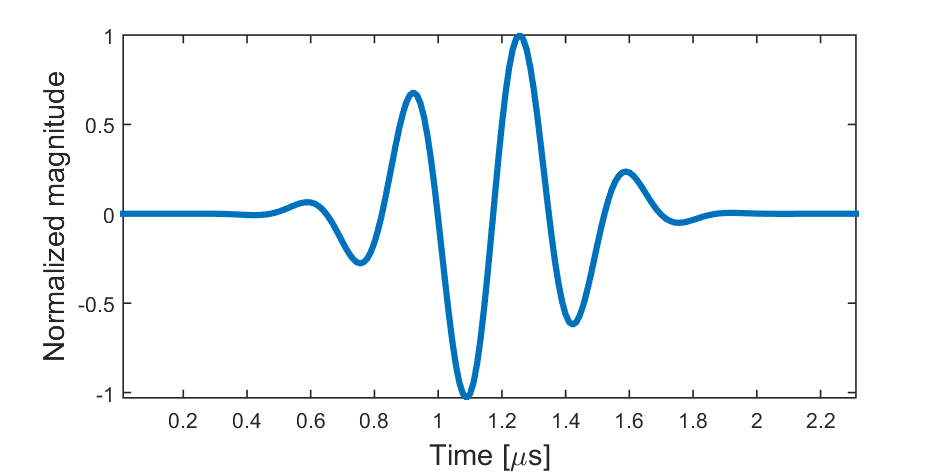
\includegraphics[width=\linewidth]{./images/others/pulse.png}
    \caption{Simulated signal pulse on reception}
    \label{fig:pulse}
\end{figure}

The imaged section is chosen to span from $-17.5$ to $17.5^\circ$ from the array's normal vector, and $35$ to $60~$mm range to it. The aperture default focus is set to $40~$mm radius. Note that this thesis differentiates the terms \textit{radius}, which defines the absolute distance to the array center in any direction, and \textit{range}, which defines the radius projection onto the array's normal plane. A point's \textit{azimuth} is its radius projection onto the array's parallel plane.

All transmit or receive beams are focused at the same radius ($40~$mm) and distributed uniformly along the imaged azimuth sector. In other words, the beams distribution is uniform in $sin(\theta_b)$, where $\theta_b$ is the direction angle of beam $b$ from the array center.
The beams with outermost direction $\theta_b$ from the array center are set to $sin(\theta_b)$ = -0.3 and 0.3.
For any given range $r$, the azimuth distance $d_B$ between two transmit beams is a constant value:
\begin{align}
    d_B = 0.3 \cdot r / \lfloor b_{tr} / 2 \rfloor,
\label{eq:dist_beams}
\end{align}
\noindent
where $b_{tr}$ is the number of beams used to illuminate the imaged sector and $\lfloor \rfloor$ is the floor operator.

Unless specified otherwise, all beamformed images are built by sequentially transmitting beams in various directions and, for each transmit beam, focusing the array towards that same direction during receive. The number of receive beams $b_{re}$ is then equal to the number of transmit beams $b_{tr}$. This approach is often referred to as single-line acquisition (SLA).
In practice, a lot of beamformers are configured to use parallel-receive beamfoming (PRB), also known as multiple-line acqusition (MLA), presented in Section \ref{sec:prb}. The purpose of PRB is to improve a beamformer's frame rate by reducing the number of transmit beams while maintaining a similar resolution level by increasing the number of receive beams.
However, this approach has shown to induce artifacts and various PRB approaches have been introduced to try to limit those artifacts (\cite{multiline}).
In order to avoid this problematic, perfect PRB is simulated in this thesis by upsampling the number of transmit beams and using SLA. Assuming perfect PRB, an image built from $b_{tr} = b_{re} = 195$ beams can therefore also be seen as built from $b_{tr} = 65$ transmit beams and $b_{re} = 3 \cdot b_{tr} = 195$ receive beams, or $b_{tr} = 39$ and $b_{re} = 5 \cdot b_{tr} = 195$ beams.

The imaged medium contains scatterer points either in a noiseless medium or in a \textit{speckle} background, depending on the experiment. Speckle noise consists of the transmitted signals scattered by a large number of small, densely distributed, scatterer points and is used to simulate homogeneous tissues.
The noiseless background scenario is a very controlled setup, with no randomness in the medium which could possibly alter the results. It is typically run first and its results are used to make fundamental observations and in-depth analysis. The speckle scenario is a more realistic one, typically used to verify the observations from the first scenario and obtain qualitative results closer to those of a real use case.
This thesis focuses on noiseless media, but provides an exposure to more realistic media with two examples of randomly-generated speckle background.
Due to the randomness of the speckle noise, a thorough analysis of the influence of motion with the presence of speckle noise would require to run the same experiments with dozens or even hundreds of different randomly-generated speckle backgrounds to be statistically meaningful.
The speckle simulations are therefore targeted to be used as examples of realistic divergences from the noiseless medium and not data of statistical significance.
In this thesis, speckle is generated by simulating one million small scatterer points uniformly distributed along the full image plane, covering -90 to 90 degrees angular span and 5 to 75 mm range.
Figure \ref{fig:speckle} displays DAS beamformed images of the two speckle backgrounds used in this thesis.

The parameters used for the aperture and medium simulation are summarized in Tables \ref{table:aperture_param} and \ref{table:medium_param}.

\begin{figure}[ht]
    \centering
    \begin{subfigure}[t]{0.48\linewidth}
        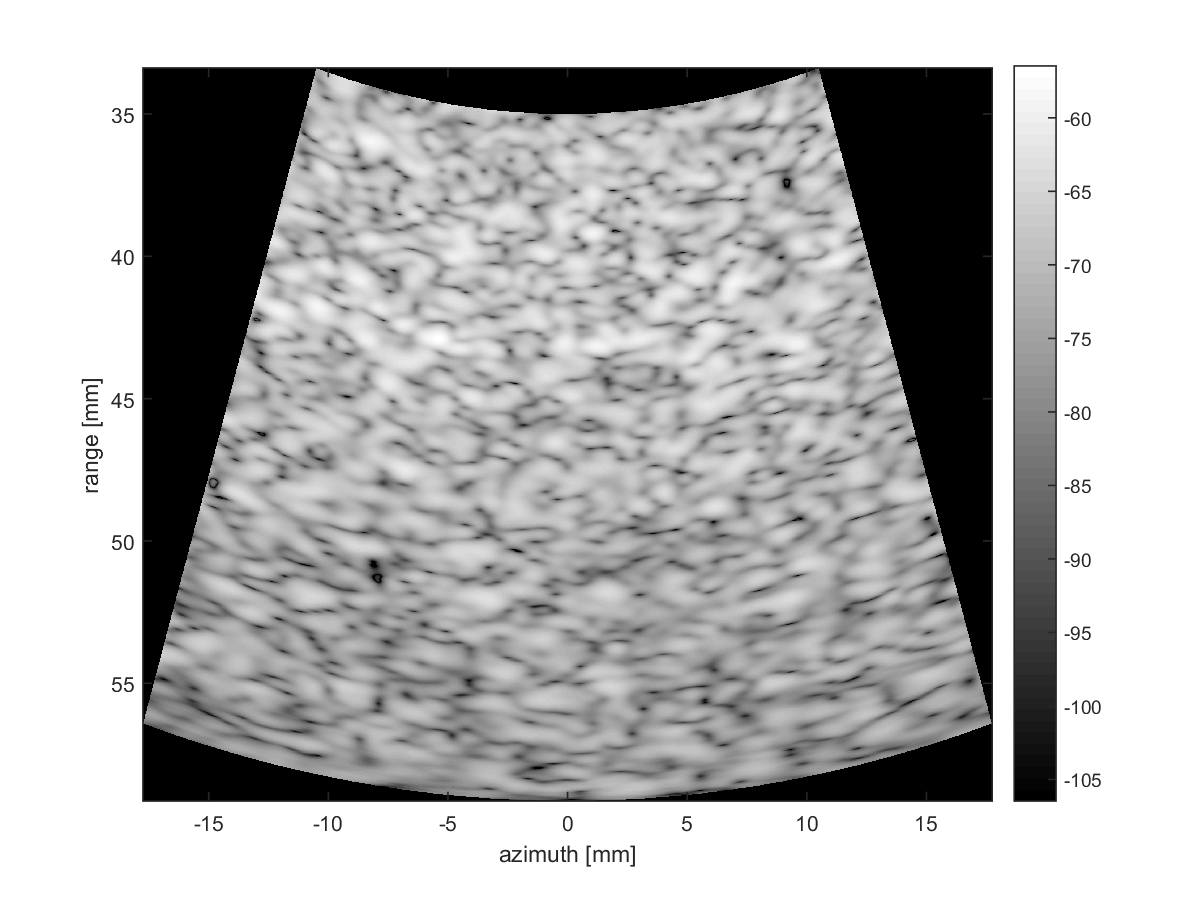
\includegraphics[width=\linewidth]{./images/results/2.3/speckle2.png}
        \caption{Speckle seed = 2}
    \end{subfigure}
    \quad
    \begin{subfigure}[t]{0.48\linewidth}
        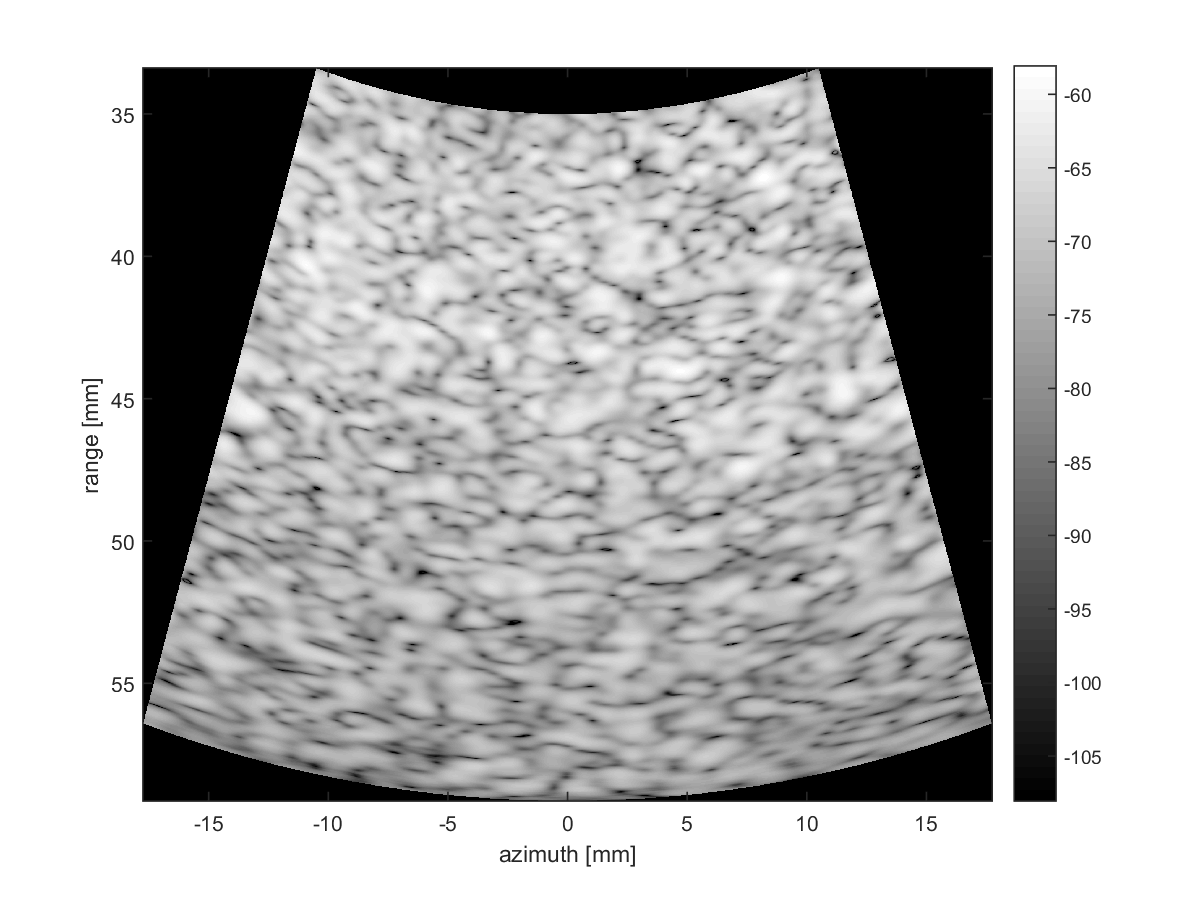
\includegraphics[width=\linewidth]{./images/results/2.3/speckle42.png}
        \caption{Speckle seed = 42}
    \end{subfigure}
	\caption{DAS beamformer image of speckle background with $b_{tr}=65$ transmit beams}
	\label{fig:speckle}
\end{figure}

\iffalse
  Recorded frequencies bandwidth    &   1.8457 - 4.1528 MHz
  along the full image plane, covering the full -90 to 90 degrees angular span.
\fi


\begin{table}[!ht]
\centering
\begin{tabular}{|*{2}{c|}}
 \hline
 \multicolumn{2}{c}{Probe parameters} \\
  \hline
  Transmit and record center frequency    &   3 MHz \\
  Transmit and record frequency bandwidth    &   2.3 MHz \\
  Sampling frequency    &   90 MHz \\
  Number of transducers &   96 \\
  Transducer height   &   10 mm \\
  Transducer width   &   0.24 mm \\
  Transducer pitch   &   0.25 mm \\
  Kerf   &   0.01 mm \\
  Array length   &   24 mm \\
  \hline
  \multicolumn{2}{c}{} \\
  
  \hline
  \multicolumn{2}{c}{Default aperture parameters} \\
  \hline
  Imaging sector  &   -17.5 to 17.5 degrees \\
  Imaging range     &   35 to 60 mm \\
  Radial focus   &   40 mm \\
  Impulse response window   &   Blackman \\
  Distribution of transmit beams   &   Uniform along azimuth \\
  Distribution of receive beams   &   Matching transmit \\
  \hline
 \end{tabular}
\caption{Probe parameters}
\label{table:aperture_param}
\end{table}
  
\begin{table}[!ht]
\centering
\begin{tabular}{|*{2}{c|}}
 \hline
 \multicolumn{2}{c}{Medium parameters} \\
  \hline
  Speed of propagation    &   1500 m/s \\
  Speckle sector    &   -90 to 90 degrees \\
  Speckle range     &   5 to 75 mm \\
  Speckle azimuth   &   -75 to 75 mm \\
  Speckle distribution  &   Uniformly distributed \\
  Number of points in speckle    &   $10^6$ \\
  Random generator seed     &   2 and 42 \\
  Scatterer points amplitude   &   30 dB over speckle \\
  \hline
 \end{tabular}
\caption{Medium parameters}
\label{table:medium_param}
\end{table} 

\section{Beamformers parameters}
\label{sec:beamform_param}
Four different beamforming algorithms are implemented and tested in this thesis:
\begin{itemize}
    \item DAS: Conventional Delay-And-Sum beamforming (Section \ref{sec:DAS})
    \item MV: Minimum-Variance beamforming (Section \ref{sec:MV})
    \item IAA-MB: Iterative Adaptive Approach (Section \ref{sec:IAA}). Two variants of the algorithm are compared:
    \subitem IAA-MBSB: (Multibeam/Singlebeam) The MB approach is used during the iteration stage and the SB approach for the final sources amplitude.
    \subitem IAA-MBMB: (Multibeam/Multibeam) The MB approach is used both during the iteration stage and the final sources amplitude estimation.
\end{itemize}
\noindent
As explained in section \ref{sec:MV}, the MV beamformer in its standard form is prone to artifacts and requires some robustification improvements. In this thesis, the MV beamformer is enhanced with the use of spatial smoothing, diagonal loading, temporal averaging and forward-backward averaging (Sections \ref{sec:diagonal_loading}, \ref{sec:spatial_smoothing}, \ref{sec:time_averaging} and \ref{sec:fb_averaging}).
Based on Figure \ref{fig:spatial_smoothing}, the subarray length value is chosen as half the array length ($96/2 = 48$). Diagonal loading and time averaging are set to relatively low values, respectively $5\%$ and +/- 2 samples, in order to keep a high MV image resolution. The time averaging value of $T=2$ means that $2T+1=5$ samples are used per range index. With a sampling frequency of 90 MHz, this corresponds to $5 / (90 \cdot 10^6) = 55.5 \cdot 10^{-9}$ seconds and, with a speed of propagation $c = 1500~$m/s, to $1500 \cdot 55.5 \cdot 10^{-9} = 83.3 \cdot 10^{-6}~$m = 0.0833 mm per range index.
For the signals transmitted at $3~$MHz, these 5 samples correspond to $5 \cdot 3 / 90 = 1/6^{th}$ of their wavelength.

The DAS and IAA beamformers are by nature more robust than MV. In this thesis, none of the for-mentioned robustification methods are applied to those beamformers. The beamspace projection concept introduced in Section \ref{sec:beamspace_projection} is however used with the IAA-MB approaches. A $M x B$ transmformation matrix, where $M$ is the number of transducers in the array and $B$ the chosen number of dimensions in the projected beamspace, is built from Equation (\ref{eq:beamspace}). The value of $B$ is obtained from Equation (\ref{eq:beamspace_size}):
\begin{equation}
    B = 2 \cdot \lceil \frac{sin(\theta_{max}) \cdot M}{2} \rceil + 1 = 2 \cdot \lceil \frac{0.3 \cdot 96}{2} \rceil + 1 = 2 \cdot 15 + 1 = 31,
\end{equation}
\noindent
where $\theta_{max}$ is the angle of the extremities of the imaged sector, set to $\pm 17.5^\circ$ in Section \ref{sec:sim_param}.

As its names suggests, the IAA approach is an iterative method, which therefore requires an iteration stop condition. The iteration steps are developed in Section \ref{sec:IAA}. The iteration stop condition can either be a fixed number of iterations, a convergence threshold or a combination of both. A fixed number of 10 iterations has been chosen in this thesis, based on empirical data from \cite{Yardibi_nonparametric_IAA} and \cite{Jensen_IAA}. Using a convergence threshold, in this case probably a threshold on how much $\boldsymbol{\hat{P}}_{qq}$ varies between two iterations (ref. Section \ref{sec:IAA}), might yield better result, but to the cost of varying computational load. This variance in number of iterations could, in extreme cases, lead to varying frame rates, which can be problematic. Furthermore, the IAA approaches have not been explored enough yet to provide reliable convergence thresholds for each variant of the beamformer.
Table \ref{table:beamformers_param} summarizes the parameters used for all beamformers.

\begin{table}[!ht]
\centering
\begin{tabular}{| c | c | c |}
  \hline
  Parameter &   Beamformer   &   Value \\
  \hline
  Subarray length   &   MV &  48 \\
  Diagonal loading  &   MV &   5 \% \\
  Forward-backward averaging    &   MV  &   Enabled \\
  Temporal averaging    &   MV  &   +/- 2 samples \\
  Beamspace projection  &   IAA &   31 \\
  Number of iterations  &   IAA &   10  \\
  \hline
 \end{tabular}
\caption{Beamformers parameters}
\label{table:beamformers_param}
\end{table}


    \chapter{Experiments}
\label{chap:experiments}

As mentioned in this thesis' introduction, adaptive beamformers have often been criticized as not reliable enough in their raw form for most active system applications such as medical ultrasound imaging.
Some of the early concerns such beamformers faced included their notable sensitivity to:
\begin{enumerate}
    \item Signal cancellation in the presence of coherent signals (\cite{van_trees})
    \item Visible artifacts in the presence of motion in the imaged medium (\cite{Asen_shift_invariance})
    \item High beam density requirements due to narrow receive beams
    \item High computational complexity prohibiting real-time ultrasound imaging
    \item High configuration complexity
\end{enumerate}
\noindent
Different approaches have been proposed to solve or limit the effect of one issue or another, some of which are presented in this thesis (Sections \ref{sec:diagonal_loading} - \ref{sec:multibeam}).
Multiple studies have compared different versions of the MV beamformers with the DAS one (\cite{Synnevag_Benefits, Synnevag_adaptive, Asen_shift_invariance}), both in idle scenarios and in scenarios exposed to motion. One objective of this thesis is to build experiments that create similar comparisons and hopefully confirm the conclusions of these publications. This aims to provide confidence in the experiments and analysis with new content.

The multibeam Iterative Adaptive Approach (IAA-MB) has been presented in ultrasound image processing by \cite{Jensen_IAA} as an alternative beamformer to MV. Although very promising, it has only been studied in medical ultrasound imaging on scenarios with stationary imaged media. The effects of motion on the IAA-MB approach is an aspect that this thesis hopes to explore and uncover.

In the domain of medical ultrasound imaging, motion in an imaged medium is often, implicitly or explicitly, defined as position shift of scatterer points from one image, or frame, to another. However, the acquisition of a single frame is not instantaneous, which means that motion within a frame is a real concept and a potential source of issues for different beamformers. This thesis aims to provide a thorough analysis of the effects of motion within frames and the resulting limitations on each beamformer.

The combined analysis of all scenarios experimented with in this thesis is expected to provide a reliable and thorough understanding of the fundamental issues and artifacts induced from motion in ultrasound imaging, along with realistic limitations, and enhancement possibilities, of each beamformer presented in this thesis.

\section{The effect of motion between frames}
\label{sec:frames_motion}
This section aims to compare how well each beamformer copes with motion between frames. \cite{Asen_shift_invariance} already revealed results comparing the MV beamformer with DAS. The goal of this section is to build on this study, hopefully confirm its findings, and provide a similar analysis for the different versions of the IAA approach presented in this thesis.

The for-mentioned study showed that the MV algorithm requires a much higher beam density than DAS in order to ensure no visible artifact. Due to the MV beams being very narrow at the radial focus, the reflections from scatterer points located in between two beams focus points can be heavily attenuated compared to scatterer points located at a beam focus point. This signal attenuation effect is known as \textit{scalloping loss} (\cite{Asen_shift_invariance}). In the case of a moving scatterer point, this scalloping loss effect will result in the point's apparent intensity varying with its position. When combining beamformed images into videos, as done for example in real-time imaging,  scatterer points in motion may appear blinking. Figure \ref{fig:bf_im} illustrates the effect of scalloping loss with the DAS beamformer. A single scatterer point is simulated in a speckle noise background. The white lines indicate transmit beams trajectories. The scatterer point starts on the center beam trajectory and is shifted half the distance between two beams per frame, such that it ends exactly on the neighboring beam trajectory in the third frame. In this example, the scatterer point is visible in frames 1 and 3, but completely disappears in the speckle background in frame 2.

\begin{figure}[ht]
    \centering
    \begin{subfigure}[t]{0.48\linewidth}
        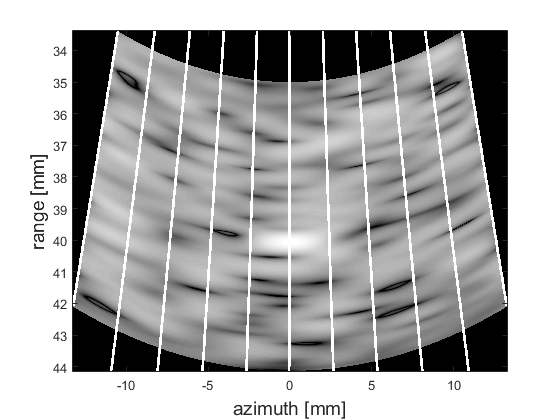
\includegraphics[width=\linewidth]{./images/others/scallop_loss1.png}
        \caption{Position of $s_1 = (0, 40)~$mm.}
        \label{fig:bf_im1}
    \end{subfigure}
    \quad
    \begin{subfigure}[t]{0.48\linewidth}
        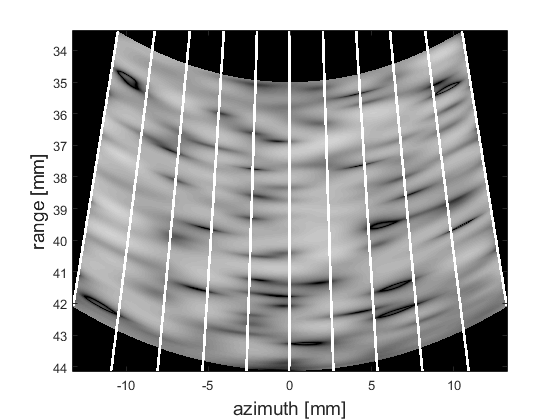
\includegraphics[width=\linewidth]{./images/others/scallop_loss2.png}
        \caption{Position of $s_1 = (1.2, 39.98)~$mm.}
        \label{fig:bf_im2}
    \end{subfigure}
    \quad
    \begin{subfigure}[t]{0.48\linewidth}
        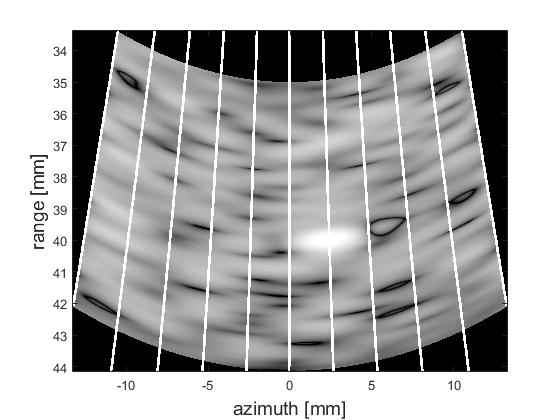
\includegraphics[width=\linewidth]{./images/others/scallop_loss3.png}
        \caption{Position of $s_1 = (2.4, 39.93)~$mm.}
        \label{fig:bf_im3}
    \end{subfigure}
    \caption[DAS beamformed images of a scatterer point $s_1$ moving in speckle.]{DAS beamformed images of a scatterer point $s_1$ moving in speckle. The scatterer point is shifted, along the beamformer's focus radius, half the distance between beams per frame. The position $(x, y)$ of $s_1$ is $(0, 40)~$mm in (a), $(1.2, 39.98)~$mm in (b) and $(2.4, 39.93)~$mm in (c), where $x$ is the offset of $s_1$ relative to the center of the array along the azimuth dimension and $y$ is the offset along the range dimension. The white lines are added on top of the beamformed image and represent the transmit beams trajectories.}
	\label{fig:bf_im}
\end{figure}

Scalloping loss, for any scatterer point in the medium, can be caused by a lack of energy transmitted towards the point's position or by signal suppression from the array towards that position.
Two of the most straightforward approaches to reducing scalloping loss are by either increasing the density of transmit beams or their width. However both methods have obvious drawbacks. The choice of beam width is a trade-off between sensitivity to scalloping loss and image resolution, whereas the choice of their density is a trade-off between sensitivity to scalloping loss and image acquisition time.

A beamformed image is considered in this thesis to be formed by sequentially transmitting and recording focused beams. Its acquisition time $t_{im}$ can be expressed in seconds as:
\begin{equation}
    t_{im} = 2 \cdot r_{max} \cdot b_{tr} / c,
\label{eq:acquisition_time}
\end{equation}
\noindent
where $b_{tr}$ is the number of transmit beams, $r_{max}$ is the maximum range in meters for which the probe is recording data and $c$, in m/s, is the speed of ultrasound propagation in the medium. The factor 2 represents the fact that active systems are used, which means that the signals need to travel to $r_{max}$ and back to the probe in order to be recorded. With $r_{max} = 0.15~$m and $c = 1500~$m/s, $t_{im} = 2 \cdot 0.15 \cdot b_{tr} / 1500 =  2 \cdot 10^{-4} \cdot b_{tr}~$seconds. A single beam transmission and acquisition is then considered to take $0.2~$ms.

Instead of acquisition time, it is often slightly more intuitive to talk about frame rate, in number of images per second, especially in the domain of real-time imaging. The beamformers' frame rate $f_{im}$ are calculated through this thesis as:
\begin{equation}
    f_{im} = 1 / t_{im} = 1 / (2 \cdot 10^{-4} \cdot b_{tr}) = 5 \cdot 10^3 / b_{tr}.
\label{eq:frame_rate}
\end{equation}
\noindent
A beamformer's frame rate is dependent on the number of transmit beams $b_{tr}$, but not dependent on the number of receive beams $b_{re}$. For beamformers using single-line acquisition (SLA), those number are equal. However, as explained in Section \ref{sec:prb}, multi-line acquisition (MLA) is an approach that can create multiple receive beams per transmit beam and output beamformed images with $b_{re} > b_{tr}$.
Given an image resolution threshold, MLA approaches can often be used to reduce the required transmit beam density compared to that of the SLA approach, thus increasing a beamformer's maximum frame rate.

Since data processing and acquisition can often be done simultaneously and computation capabilities are constantly increasing, we focus in this thesis on analyzing delays due to data acquisition and assume data processing can be made such that it does not result in additional delays.
In order to avoid potential artifacts, the whole imaged medium is considered to be idle within a single frame. The effects of motion within frames are studied in Section \ref{sec:beams_motion}.

In order to give a meaningful interpretation of the effects of scalloping loss, and qualitatively compare these results with previous studies, the scalloping visibility threshold is taken from \cite{Asen_shift_invariance}: \newline
\textit{In an ultrasound image with 50dB dynamic range mapped to 256 gray levels, a 1dB loss corresponds to 5 gray levels. This is approximately equal to the visibility threshold [Weber fraction of 2\%] for grayscale images. A loss larger than 1dB could therefore end up being visible to the observer.}

Since focused beams are by definition the narrowest at their radial focus, it is the range at which the scalloping loss of scatterer points is expected to be the most severe. This assumption has to be verified before comparing beamformers performance at radial focus.
To simulate the highest possible scalloping loss, the scatterer point motion follows the aperture's focus radius and is therefore physically a circular motion. Multiple frames are recorded with the point at different angles from the aperture's center. The maximum scatterer point gain is expected to be recorded when its angle matches one of the array's beams. Its minimum gain is expected to be recorded when its angle is exactly in between two beams angle. The scatterer point maximum scalloping loss is then calculated by subtracting its estimated minimum gain to its estimated maximum gain.


\section{The effect of motion within frames}
\label{sec:beams_motion}
In Section \ref{sec:frames_motion}, the back-scattered image was assumed to be still within each frame. This section is analyzing the effects of motion within a single frame. This domain has been very little studied so far in medical ultrasound imaging, which makes it harder to predict the outcome of such experiments. However this might hint that motion within frames has not revealed any known major issue for conventional beamformers and might only induce negligible errors in the beamformers model. The purpose of this section is to analyze the effects of such motion and give sensible information about how robust the different beamformers are in realistic scenarios.

The domain of photography, although fundamentally different in its signal acquisition process from ultrasound beamforming, is dramatically affected by motion within frames. Almost anybody who has ever handled a camera has experienced motion in the imaged scenery leading to blur in the image. This experience, perhaps misleadingly, directs us to expect such motion in the ultrasound imaging domain to result in distortions of the scatterer points shape and amplitude.

In order to give more insightful predictions, it is worth analyzing the photography analogy a bit deeper. First of all, cameras capture frames by recording light waves simultaneously for the whole spatial spectrum. The reason blur or artifacts can appear is that the frame's capture is not instantaneous. The camera's \textit{exposure time} is what defines how long a frame is recorded for. A long exposure time allows us to record a lot of light and get brighter pictures. A short exposure time limits the effects of motion blur, but also results in darker pictures. This process can be seen as continuously taking instantaneous frame for a given period and produce the final picture by averaging those frames. If an object moves during that time, it can appear blurry since not at the same spatial location for all frames. Motion in any direction would then result in the object appearing bigger than if idle. 

In ultrasound imaging, the probes are typically sending short pulses which are reflected by scatterers in the imaged medium. In such scenarios, with only a few samples per range pixel, motion in the medium within a single beam is way beyond human perception for velocities $v << c$, the speed of ultrasound propagation, and can be ignored. However, blur and artifacts can occur due to the sequential nature of image acquisition, i.e. the formation and recording of directional beams. Frames are produced by transmitting and recording directional beams along the imaged spatial spectrum. In this thesis, the beams are transmitted sequentially from negative to positive degrees/azimuth. Each beam needs to propagate until the desired maximum image range and back to the array before another beam can be transmitted. The image acquisition time is defined by Equation (\ref{eq:acquisition_time}).

In the photography analogy, it would be similar to taking a panoramic picture, where picture frames are extended by other ones in order to form a picture with extended spatial range. Assuming this time that each picture is instantaneous, no blur or artifact can occur within a single picture. For simplicity, it is first considered that all pictures are forming a perfectly aligned panoramic picture, with no overlap in their imaged sector. Multiple scenarios of a single object moving in a stationary background are then proposed in Table \ref{table:panoramic_perfect}, where the object motion $\boldsymbol{m_o}$ is expressed relative to the panoramic picture acquisition direction $\boldsymbol{m_p}$.

With these initial intuitions in mind, the photography analogy can be extended to the scenario for which the different pictures overlap in their imaged sector. The same scenes as Table \ref{table:panoramic_perfect} are analyzed with pictures overlap in Table \ref{table:panoramic_imperfect}.

\begin{table}[!ht]
\centering
\begin{tabular}{| c | c |}
  \hline
  \textbf{Scenario}  &   \textbf{Expected result} \\
  \hline
  Object appears only in one frame    &   No artifact or blur \\
  \hline
  $\boldsymbol{m_o}$ in same direction as $\boldsymbol{m_p}$  &  The object can appear dilated, or, in \\
    &  extreme cases, a duplicate can appear \\
  \hline
  $\boldsymbol{m_o}$ opposite to $\boldsymbol{m_p}$    &  The object can appear eroded   \\
    &   or, in extreme cases, disappear \\
  \hline
  $\boldsymbol{m_o}$ perpendicular to $\boldsymbol{m_p}$    &   The object can appear distorted \\
  \hline
 \end{tabular}
\caption{Photography analogy of an object moving in between frames of a panoramic picture. Expected artifacts with perfect image segmentation.}
\label{table:panoramic_perfect}
\end{table}


\begin{table}[!ht]
\centering
\begin{tabular}{| c | c |}
  \hline
  \textbf{Scenario}  &   \textbf{Expected result} \\
  \hline
  Object appears only in one frame    &   No artifact or blur \\
  \hline
    &  The object can appear blurry, \\
  $\boldsymbol{m_o}$ in same direction as $\boldsymbol{m_p}$  &   dilated or, in extreme cases,  \\
    &   a duplicate can appear   \\
  \hline
  $\boldsymbol{m_o}$ opposite to $\boldsymbol{m_p}$    &  The object can appear \\
    &   blurry or eroded  \\
  \hline
  $\boldsymbol{m_o}$ perpendicular to $\boldsymbol{m_p}$    &   The object can appear \\
    &   blurry or distorted \\
  \hline
 \end{tabular}
\caption{Photography analogy of an object moving in between frames of a panoramic picture. Expected artifacts with imperfect image segmentation.}
\label{table:panoramic_imperfect}
\end{table}

The first part of this section aims to give a first exposure to the effects and possible issues of motion within frames. The assumptions of Tables \ref{table:panoramic_imperfect} and \ref{table:panoramic_perfect} made from the photography analogy are then compared to the results in medical ultrasound imaging. Different motion patterns and velocities are studied with a single scatterer point at the array's focus range, in a noiseless background. Then, the same analysis is done with the presence of speckle noise, in order to confirm or disprove the conclusions made from the first analysis.

Blood flow velocities in arteries are typically on average around 0.12 m/s, with peaks around 0.6 m/s (\cite{Blood_flow}). With this in mind, this section's analysis focuses on the 0 to 0.6 m/s velocity range.
The second part of this section analyses the effect of motion with multiple scatterer points in an attempt to discover any potential additional effect in scenarios with coherent signals. The experiments run are very similar to those of the first part of this section, although with the presence of signal coherence induced by two closely-separated scatterer points in the imaged medium.

    \chapter{Results and Discussion}
\label{chap:results}
\section{The effect of motion between frames}
\label{sec:res_frames_motion}
In this thesis, we explore the effects of tissue motion mainly with worst case scenarios. We believe this allows for more straightforward analyses and results bound by physical constrains rather than arbitrary ones.
The first part of this section aims to define what a worst case scenario consists of.

The first experiment simulates two scatterer points, $s_1$ and $s_2$, at $40~$mm, respectively $55~$mm, distance to the transducer array in an a noiseless medium. Multiple image frames are created with the scatterer points at different angles from the array's normal vector. Each image is built from $b_{re} = b_{tr} = 11$ transmit and receive beams. The first frame has $s_1$ and $s_2$ located at angle $\theta = -3.44^\circ$, which corresponds to the angle of focus of one of the transmit beams. Then 16 additional frames are built with the scatterer points shifted 1/8th of the angular separation between two beams. This means that, in the first, middle and last frames, both scatterer points are on the trajectory of a transmit beam. An illustration of the transmit beams trajectories and the scatterer points position is provided in Figure \ref{fig:frames_illustration}. The vertical and diagonal lines represent the trajectory of transmit beams for each frame, and the ellipses represent the set of scatterer points positions for all frames combined.
Notice that the points' range varies with angular shift so that they always remain at the same radius, i.e. distance to the array's center.

\begin{figure}[ht]
    \centering
    \begin{subfigure}[t]{0.48\linewidth}
        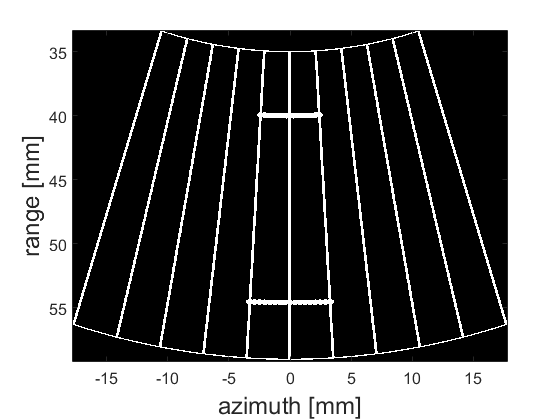
\includegraphics[width=\linewidth]{./images/results/1/illustration_scene.png}
    \caption{Illustration of whole scene}
    \label{fig:image_illustration}
    \end{subfigure}
    \quad
    \begin{subfigure}[t]{0.48\linewidth}
        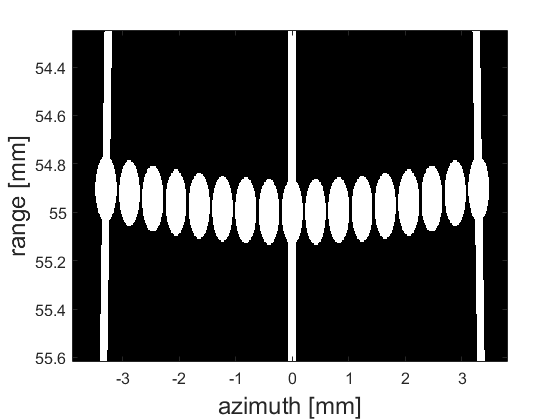
\includegraphics[width=\linewidth]{./images/results/1/zoom_55mm.png}
    \caption{Zoom around $55~$mm range}
    \label{fig:image_illustration_zoom}
    \end{subfigure}
	\caption{Illustration of imaged scene with 11 transmit beams and two scatterer points at $40~$mm and $55~$mm radius}
	\label{fig:frames_illustration}
\end{figure}

For each raw image, all four beamformers presented in Section \ref{sec:beamform_param} are used to produce a different beamformed image. As example of beamformed images, 2 of the 17 DAS beamformed frames are displayed in Figure \ref{fig:DAS_frame}, one with the scatterer points aligned with a beam trajectory ($0~$mm azimuth) and the other with the scatterer points in between two beams ($1.2~$mm and $1.65~$mm azimuth). Both scatterer points have lower apparent gain in Figure \ref{fig:DAS_frame2} than in Figure \ref{fig:DAS_frame1}.
Note that all the beamformed images displayed in this thesis are interpolated to yield smoother displays.
Although image interpolation is common practice before display, it is not applied to any the raw data in order to avoid any potential artifact that could disturb the analysis.

\begin{figure}[ht]
    \centering
    \begin{subfigure}[t]{0.48\linewidth}
        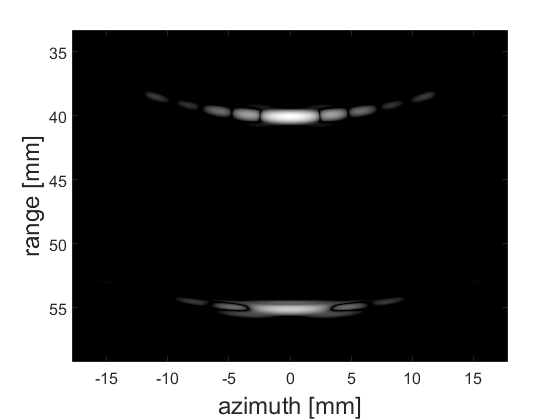
\includegraphics[width=\linewidth]{./images/results/1/DAS_frame1.png}
        \caption{Scatterer points at $0~$mm azimuth}
        \label{fig:DAS_frame1}
    \end{subfigure}
    \quad
    \begin{subfigure}[t]{0.48\linewidth}
        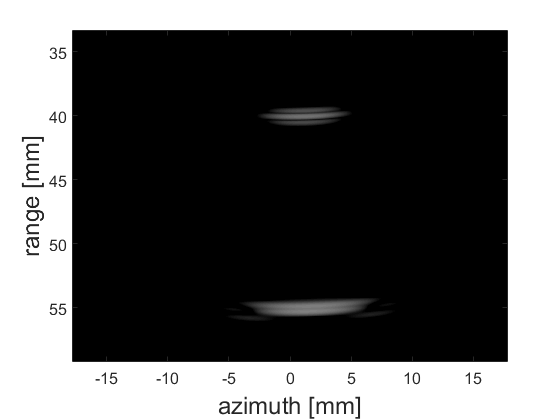
\includegraphics[width=\linewidth]{./images/results/1/DAS_frame2.png}
        \caption{Scatterer points at $1.2~$mm and $1.65~$mm azimuth}
        \label{fig:DAS_frame2}
    \end{subfigure}
	\caption{DAS beamformed image with 11 transmit beams and two scatterer points at $40~$mm and $55~$mm radius}
	\label{fig:DAS_frame}
\end{figure}

The variation in the backscattered signals gain is caused by scalloping loss, as explained in Section \ref{sec:beams_motion}. In this first experiment, for each beamformed image, the gain of the signals backscattered by each scatterer point is extracted and used for analysis.
The resulting gains are displayed in Figure \ref{fig:loss_vs_shift}.
Since the target of analysis is the difference in signal gain and not their absolute value, all gain values are normalized to that of the first frame.
Multiple observations can be made from these results. First of all the MV algorithm experiences much heavier scalloping loss than DAS in this example.
This is expected from the ability of the MV beamformer to form narrow receive beams compared to those of DAS.
This ability is the reason for the MV beamformer to be originally referred to as a high-resolution beamformer and is also the source of its increased sensitivity to angular undersampling compared to DAS.
Perhaps surprisingly, the IAA beamformers, also able to form narrow receive beams, are experiencing scalloping loss of lower or equal magnitude than DAS.
We do not want to draw conclusions based on a single experiment, but it seems at least in that example that the multibeam approach is effective in compensating for scalloping loss with angular undersampling.

As mentioned in Section \ref{sec:frames_motion}, in this thesis scalloping loss is considered invisible (and therefore negligible) if of magnitude lower or equal to 1 dB. 
A second observation is that, for all beamformers, the recorded gain of the scatterer points consistently appears to be maximized when they are aligned with a transmit beam and minimized when exactly in between two beams.
Given these results and the definition of \textit{scalloping loss} in Section \ref{sec:frames_motion}, the following experiments assume the maximum scalloping loss of a scatterer point to be its gain difference when aligned with a transmit beam and when exactly in between two beams. For example, the maximum scalloping loss of the MV beamformer for the scatterer point at $40~$mm radius is $43.2~$dB.

\begin{figure}[ht]
    \centering
    \begin{subfigure}[t]{\linewidth}
        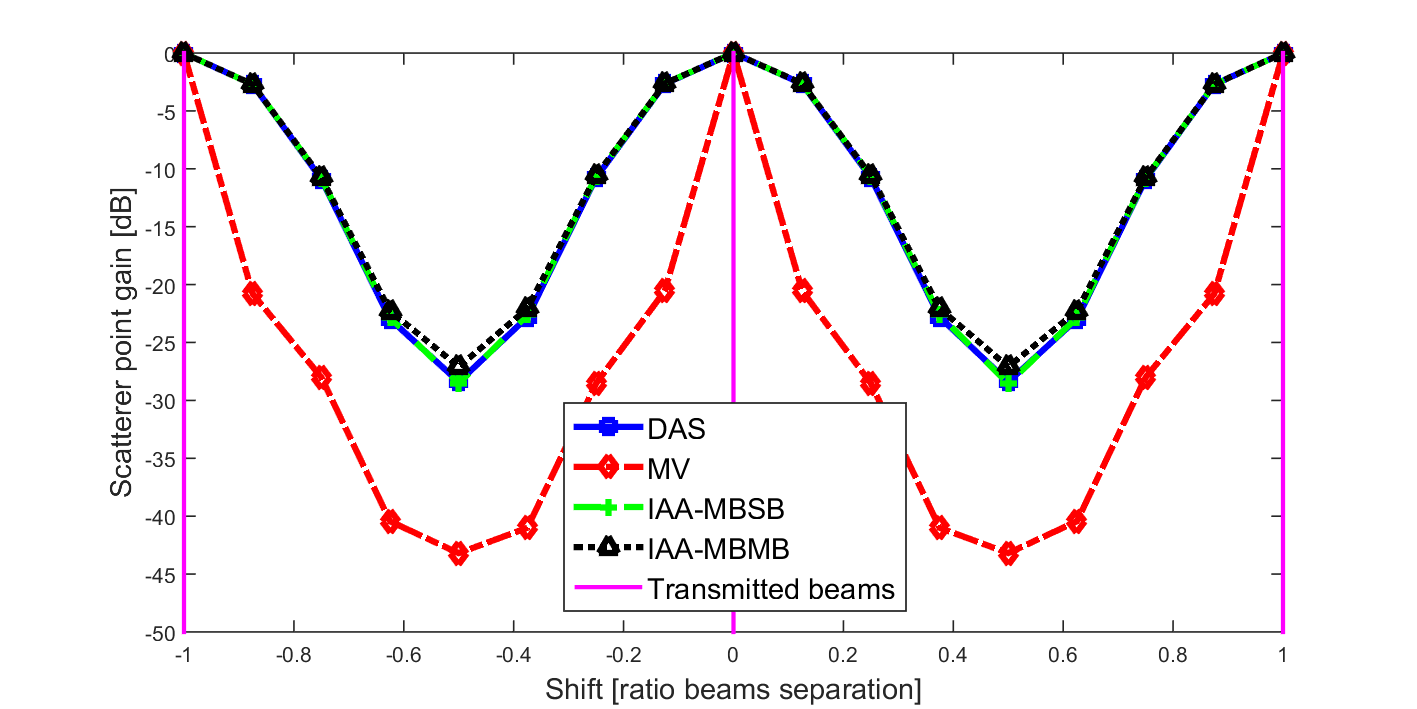
\includegraphics[width=\linewidth]{./images/results/1/loss_vs_shift_40mm.png}
        \caption{Scatterer point at $40~$mm radius}
    \end{subfigure}
    \quad
    \begin{subfigure}[t]{\linewidth}
        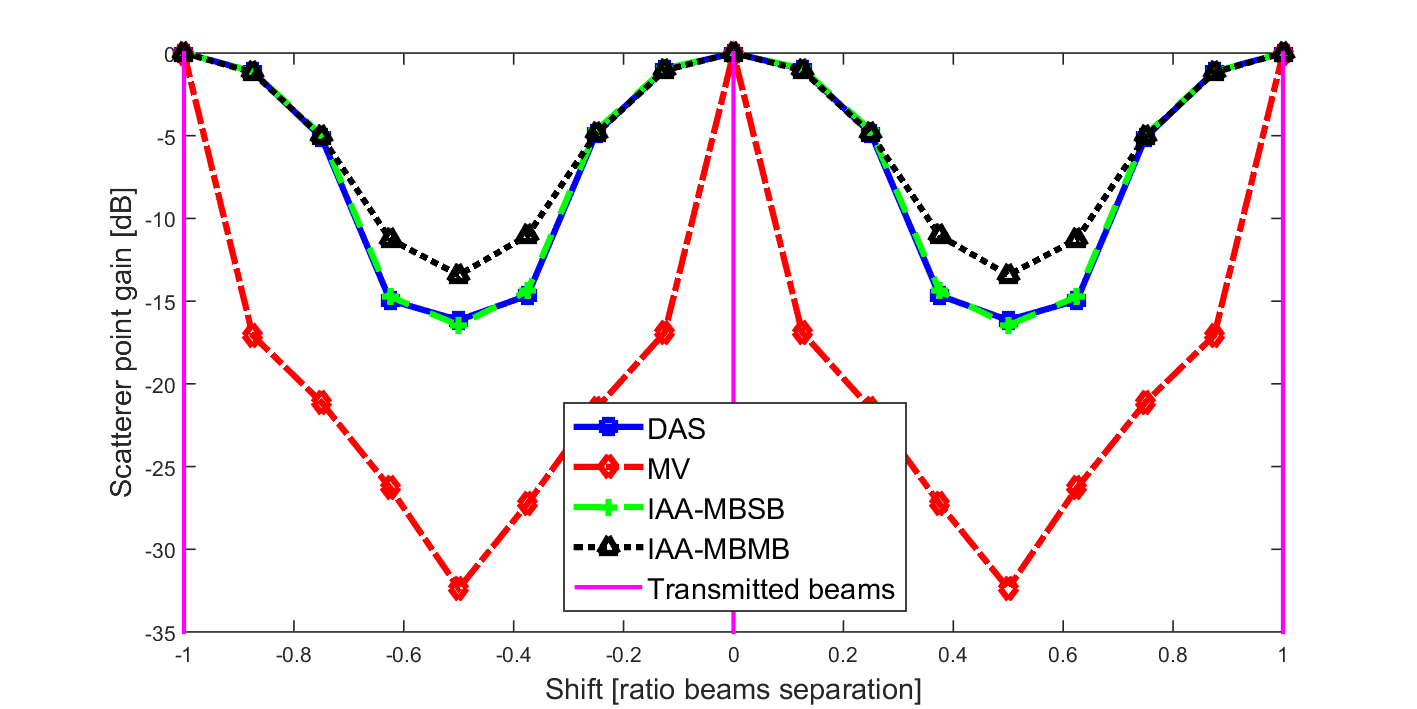
\includegraphics[width=\linewidth]{./images/results/1/loss_vs_shift_55mm.png}
        \caption{Scatterer point at $55~$mm radius}
    \end{subfigure}
	\caption{Normalized backscattered gain of scatterer point shifted 1/8th of the distance between beams per frame}
	\label{fig:loss_vs_shift}
\end{figure}


A final observation is that scalloping loss is more severe at $40~$mm radius than $55~$mm for all beamformers. In Section \ref{sec:frames_motion}, we emitted the hypothesis that scalloping loss can potentially be more severe at the array's focal distance than at any other radius.
In order to confirm that hypothesis, we set up an experiment similar to the previous one with a single scatterer point $s_1$ at various distances from the array, ranging from $36$ to $56~$mm radius.
For every given radius, we create two frames; one with $s_1$ aligned with the array's center transmit beam, at $0^\circ$ angle, and another frame with $s_1$ shifted along the same radius value so that it is placed exactly in between two beams.
For each beamformer and radius value, the scatterer point's recorded gain difference between the two frames defines its maximum scalloping loss.
The results of that experiment, displayed in Figure \ref{fig:loss_vs_range}, confirm the hypothesis that the scalloping loss is most severe at the array's focal distance ($40~$mm radius).
The magnitude of scalloping loss experienced by the IAA approaches are again lower or roughly equal to that of DAS.
\begin{figure}[ht]
    \centering
    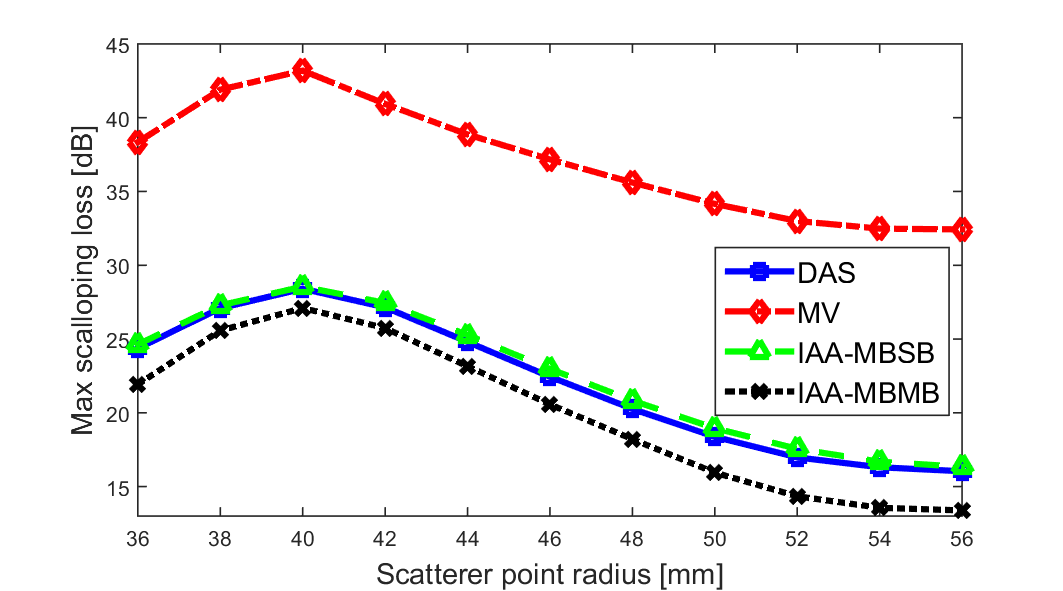
\includegraphics[width=\linewidth]{./images/results/1/loss_vs_range.png}
	\caption{Maximum scalloping loss of single point moving at constant radius}
	\label{fig:loss_vs_range}
\end{figure}

We are now able to define a worst case scenario regarding scalloping loss. The highest scalloping loss is expected to occur along the array's focus distance, assuming that the array's transmit focus line and receive focus line are the same.
Also assuming single-line acquisition (SLA), the highest scalloping loss for any given radius is expected to occur exactly in between two beams.
The highest scalloping loss magnitude is obtained in this thesis by simulating a scatterer point located at the array's focus distance ($40~$mm radius) and in between the array's center beam and its closest one towards the positive angle/azimuth values.
The following experiment recreates this worst case scenario with a noiseless medium.

We stated in Section \ref{sec:frames_motion} that there is an obvious dependence of the scalloping loss magnitude on the array's beam density and width.
We expect from \cite{Asen_shift_invariance} that scalloping loss can be reduced by increasing either the transmit and receive beam density and/or width.
Since the choice of beam width is a trade-off between angular sampling and image resolution, we prefer to focus on the choice of beam density in this section.
The transmit beam density gives a trade-off between angular sampling and image frame rate. We first focus on SLA beamforming.
For each transmit beam density $b_{tr}$, the maximum scalloping loss of each beamformer is recorded and displayed in Figure \ref{fig:loss_vs_beams}.

The DAS beamformer requires at least 65 beams to guarantee no visible scalloping loss in the imaged scene. Since the same algorithm is used for all beamformers for beams transmission, this number can be taken as basis for the required number of transmit beams $b_{tr}$. We think that the other beamformers can then achieve non-visible scalloping loss with $b_{tr} = 65$ by using parallel receive beamforming (PRB, Section \ref{sec:prb}). This can be done by creating multiple receive beams per transmit beam.
In this thesis, the beamformed images are obtained by sequentially transmit beams and, for each transmit beam, create a single receive beam aimed at the same focus point.
The perfect receive beam reconstruction is simulated by simply increasing the number of transmit beams so that $b_{tr} = b_{re}$.
Scalloping loss can obviously also be attenuated by simply increasing $b_{tr}$, but this results in an increased image acquisition time and therefore reduced frame rate. The transmit beam density is therefore always kept as low as possible.
The transmit beam density could be set even lower by increasing their width, but this would result in a resolution loss, as explained in Section \ref{sec:frames_motion}. 

As expected from Figures \ref{fig:loss_vs_shift} and \ref{fig:loss_vs_range}, the MV beamformer requires a much higher beam density than the other beamformers.
At the end of this section, we show an extension of the MV beamformer with higher beam densities until invisible scalloping loss is achieved.
As expected from the previous experiments, the IAA-MB approaches are experiencing lower scalloping loss than DAS at low beams densities ($b_{re} < 35$ for IAA-MBSB and $b_{re} < 31$ for IAA-MBMB), but experience higher scalloping loss at higher beams densities. They require a higher beams density that DAS to avoid visible scalloping loss. This shows that the multibeam approach is good at attenuating major scalloping losses, by combining the information contained in several beams. However, since the IAA approaches are high-resolution beamformers, any remaining scalloping loss not corrected by the multibeam approach can be of higher magnitude than DAS due to the difference in their steered response mainlobe width.

\begin{figure}[ht]
    \centering
    \begin{subfigure}[t]{\linewidth}
        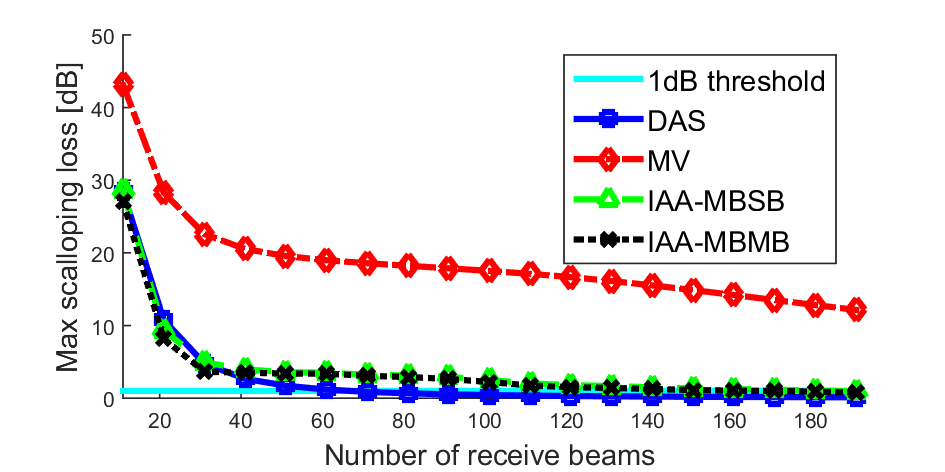
\includegraphics[width=\linewidth]{./images/results/1/loss_vs_beams.png}
        \caption{Whole plot}
    \end{subfigure}
    \quad
    \begin{subfigure}[t]{\linewidth}
        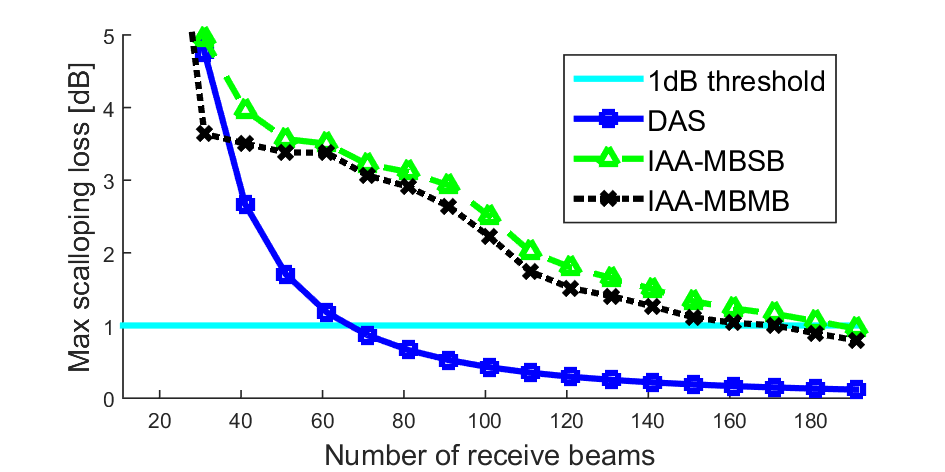
\includegraphics[width=\linewidth]{./images/results/1/loss_vs_beams_zoom.png}
        \caption{Plot focus on $[0, 5]~$dB range}
    \end{subfigure}
	\caption{Maximum scalloping loss of single scatterer point at $40~mm$ radius in noiseless medium}
	\label{fig:loss_vs_beams}
\end{figure}

The same experiment is then done on an imaged section containing speckle. Since speckle noise introduces randomness in the imaged medium, the same experiment is done with two different randomness generator seeds, $2$ and $42$.
Since a background with speckle noise is not smooth, different resolution cells can have different values, which means that a beamformer's maximum scalloping loss can not be estimated as done previously. The experiment displayed in Figure \ref{fig:loss_vs_shift} is reiterated here with a speckle background and displayed in Figure \ref{fig:loss_vs_shift_speckle}. The results show that the scatterer point minimum gain is not guaranteed to be exactly in between two beams anymore, due to the randomness of the background level. For that reason, for a given beam density $b_{tr}$, four frames are created with a single scatterer point shifted 1/4th of the angular distance between two beams per frame. Note that this does not guarantee to obtain the maximum possible scalloping loss, but it is considered in this thesis as good enough for the targeted accuracy. Those speckle simulations are indeed targeted to be used as examples of realistic divergences from the noiseless medium. Accurate analysis of speckle media would not only require a much higher number of frames per simulation, but also many more speckle background example in order to obtain meaningful statistical data. The scale of added computations and workload puts this out of the scope of this thesis.
\begin{figure}[ht]
    \centering
    \begin{subfigure}[t]{\linewidth}
        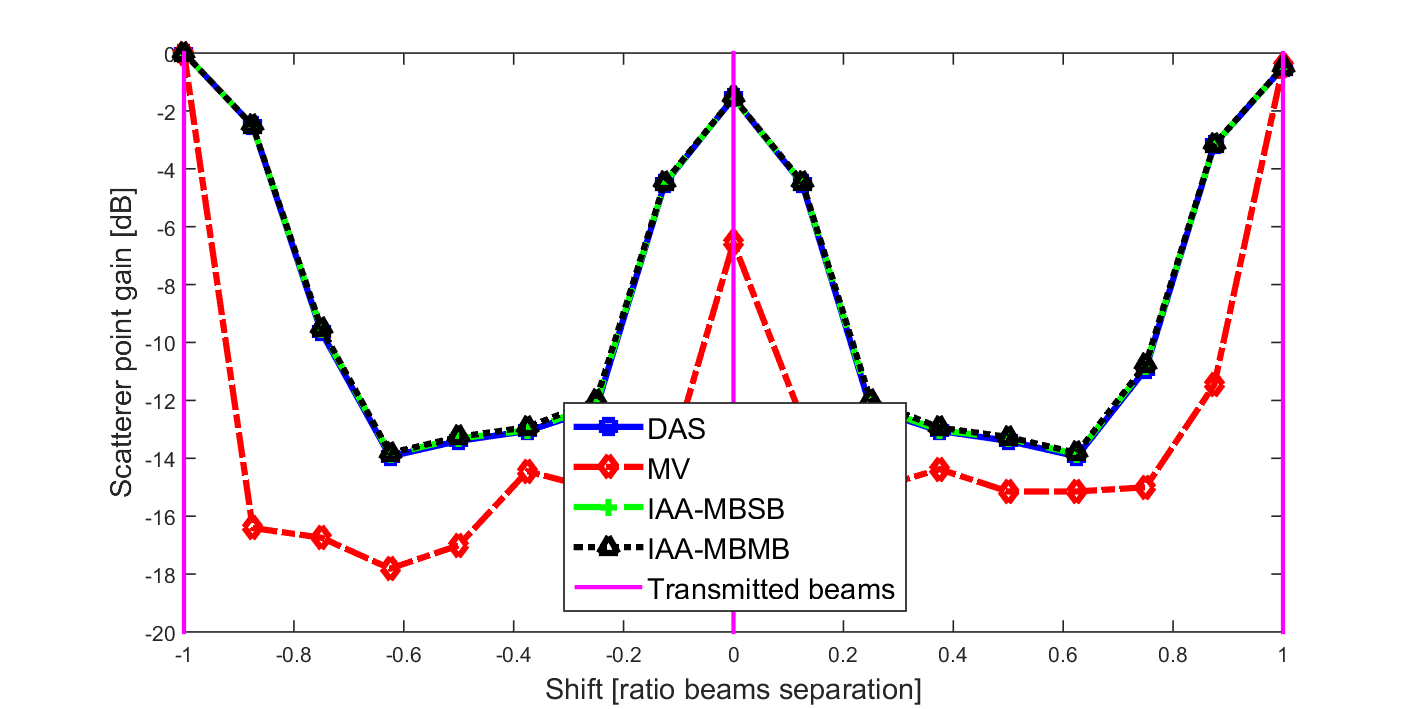
\includegraphics[width=\linewidth]{./images/results/1/loss_vs_shift_40mm_speckle.png}
        \caption{Scatterer point at $40~$mm radius}
    \end{subfigure}
    \quad
    \begin{subfigure}[t]{\linewidth}
        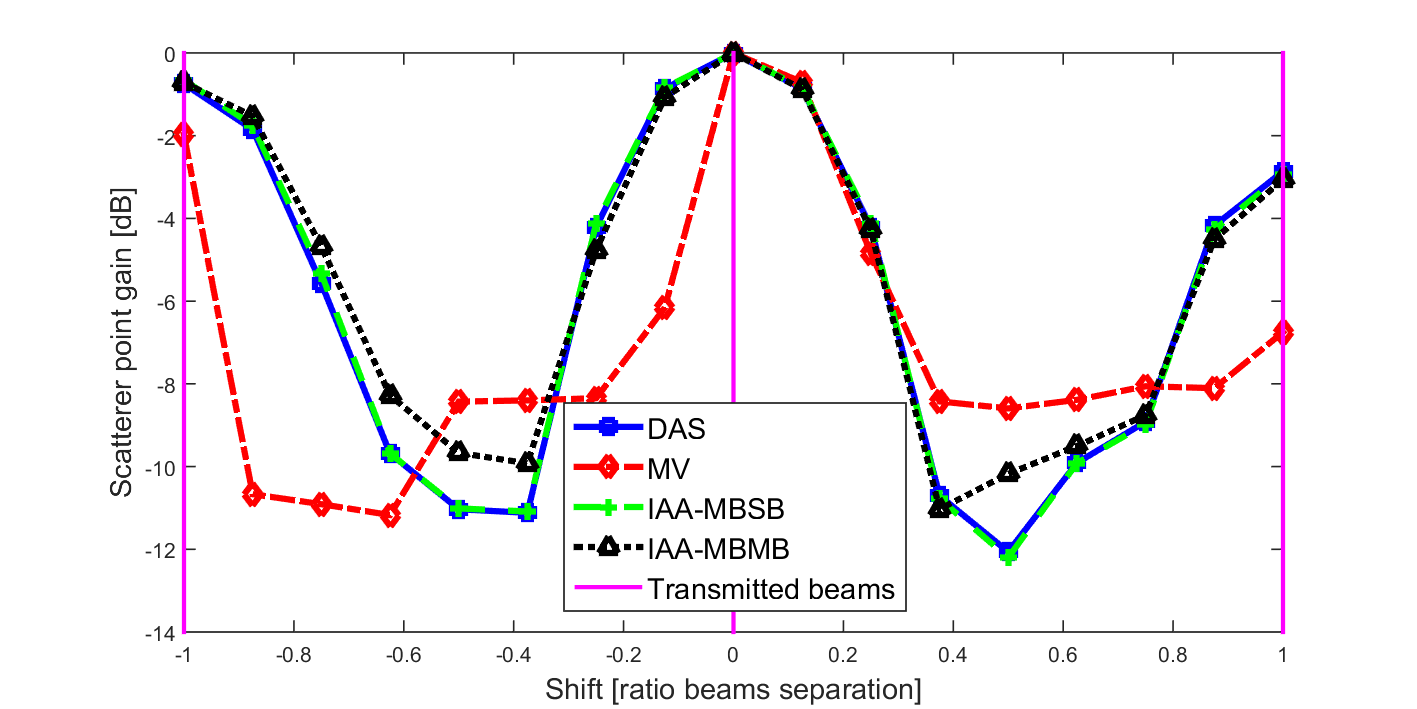
\includegraphics[width=\linewidth]{./images/results/1/loss_vs_shift_55mm_speckle.png}
        \caption{Scatterer point at $55~$mm radius}
    \end{subfigure}
	\caption{Normalized gain of scatterer point shifted 1/8th of distance between beams per frame in speckle background}
	\label{fig:loss_vs_shift_speckle}
\end{figure}

With the new approach to maximum scalloping loss estimation, the next experiment simulates a medium with speckle noise and a scatterer point at $40~$mm radius. The experiment is run with the two speckle backgrounds generated. The results are displayed in Figure \ref{fig:loss_vs_beams_speckle}.
As observed in the previous experiments, the MV algorithm experiences much heavier scalloping loss than the other beamformers. The IAA algorithm performs very well for an adaptive method, but some scalloping loss can still be visible for low beam densities. Another interesting observation is that the adaptive beamformers are more sensitive to the medium properties than the DAS one. They are sensitive to the presence of speckle noise and are consistently requiring fewer transmit beams to guarantee no visible scalloping loss.
This can easily be explained by the adaptive nature of the beamformers steered response. Adaptive beamformers can take advantage of directions towards which no or little energy is recorded and build steered responses with big sidelobes along those directions if it helps to build a higher and narrower mainlobe. The noiseless scenario can therefore produce globally narrower mainlobes, which results in an increase in their required density to avoid visible scalloping loss.
\begin{figure}[ht]
    \centering
    \begin{subfigure}[t]{\linewidth}
        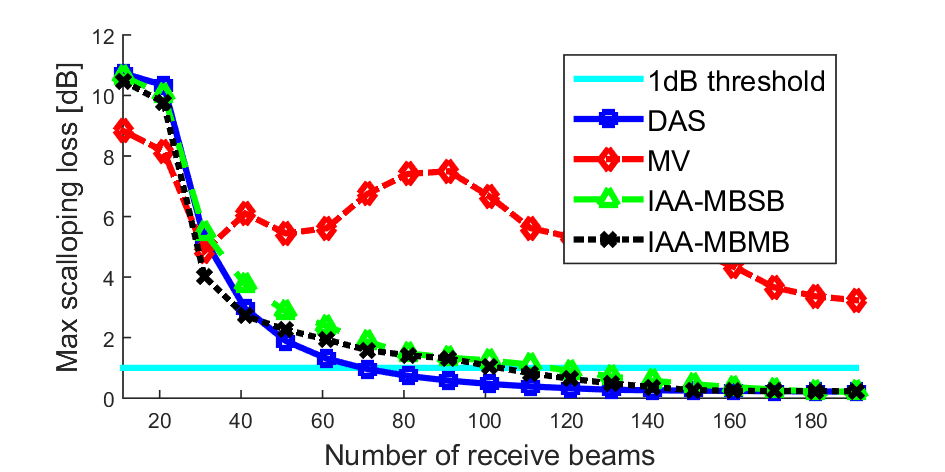
\includegraphics[width=\linewidth]{./images/results/1/loss_vs_beams_speckle2.png}
        \caption{Speckle seed 2}
    \end{subfigure}
    \quad
    \begin{subfigure}[t]{\linewidth}
        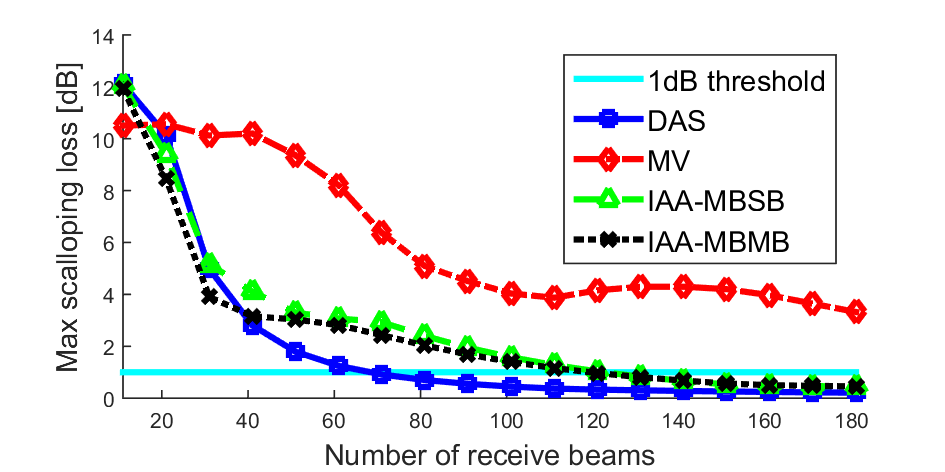
\includegraphics[width=\linewidth]{./images/results/1/loss_vs_beams_speckle42.png}
        \caption{Speckle seed 42}
    \end{subfigure}
	\caption{Maximum scalloping loss of single scatterer point at $40~$mm radius in speckle noise}
	\label{fig:loss_vs_beams_speckle}
\end{figure}

The required number of receive beams for each beamformer is summarized in Table \ref{table:num_beams}. The numbers for the MV beamformer are obtained from extending $b_{re}$ up to 981. An extension of Figures \ref{fig:loss_vs_beams} and \ref{fig:loss_vs_beams_speckle} for the MV beamformer is displayed in Figure \ref{fig:loss_vs_beams_ext}.
It is worth mentioning that 981 beams for 35 degrees coverage is well above typical beam densities and, even assuming that perfect PRB with $b_{re} > 15 \cdot b_{tr}$ is doable, such a high number of receive beams may cause significant computational delays.
In practice, the required receive beam density may have to be reduced. This can be achieved to the cost of reduced resolution by for example increasing the diagonal load and/or by creating wider receive beams.

\begin{figure}[ht]
    \centering
        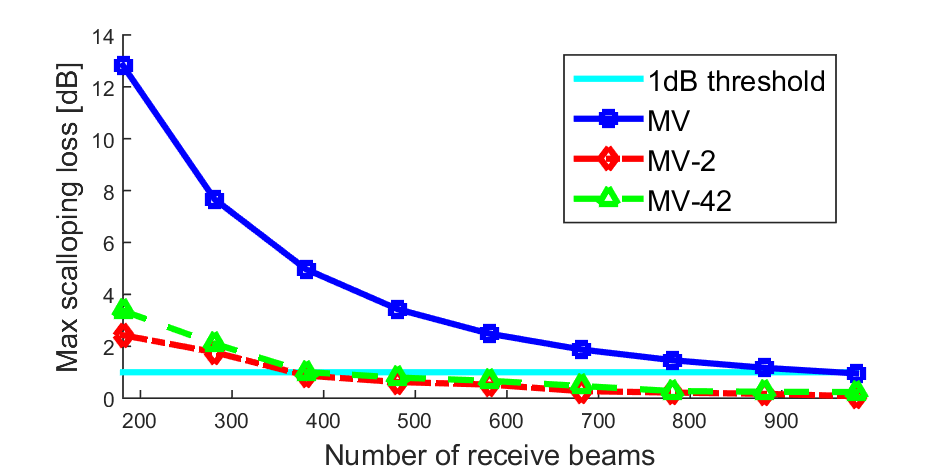
\includegraphics[width=\linewidth]{./images/results/1/loss_vs_beams_ext.png}
	\caption{MV Maximum scalloping loss of single scatterer point at $40~$mm radius in different media. MV is in noiseless medium, MV-2 and MV-42 in speckle noise (Seed 2, respectively 42)}
	\label{fig:loss_vs_beams_ext}
\end{figure}

\begin{table}[!ht]
\centering
\begin{tabular}{| c | c | c | c |}
  \hline
  Beamformer &   Without speckle   &   Speckle - seed 2 &   Speckle - seed 42 \\
  \hline
  DAS       &   65      &   71  &   71   \\
  MV        &   981     &   381  &   381 \\
  IAA-MBSB  &   191     &   101  &   123  \\
  IAA-MBMB  &   173     &   101 &   121  \\
  \hline
 \end{tabular}
\caption{Required number of beams for non-visible scalloping loss}
\label{table:num_beams}
\end{table}

As explained in Section \ref{sec:frames_motion}, the number of transmit beams has an impact on the beamformer's maximum frame rate. With $b_{tr} = 65$, the acquisition time of a single image can be obtained from Equation (\ref{eq:acquisition_time}): $t_{im} = 2 \cdot 0.15 \cdot 65 / 1500 = 13~$ms. In terms of frame rate (Equation (\ref{eq:frame_rate})), this results in a maximum of $f_{im} = 10^4 / (2 \cdot 65) = 76.9$ frames per second.
It is however important to mention that all images produced in this thesis are relatively small, only $2.5~$cm range and $35^\circ$ angular extent, and only are only produced with beams focused at the same radius ($40~$mm). In many applications, bigger images are produced by creating beams with various focal radius. Many applications create images by sequentially transmitting and recording focused beams with a constant focal radius, such as done in this thesis, and repeat the sequence with a new focal radius. Each sequence is often referred to as a \textit{line of focus}. For images with multiple lines of focus, the maximum frame rate can be estimated to that of an image with single line of focus divided by the number of lines of focus.


\iffalse
As explained in Section \ref{sec:frames_motion}, the number of transmit beams has an impact on the beamformer's maximum frame rate. Table \ref{table:max_frame} combines the results of Table \ref{table:num_beams} and Equation \ref{eq:frame_rate}.

\textbf{What kind of frame rate is acceptable for real-time imaging?}

The MV beamformer requires too many transmit beams to both be used in real-time imaging and avoid visible scalloping loss. It is worth mentioning that 981 beams for 35 degrees coverage is well above typical beam densities and such a high number of beams would, on top of the physical acquisition delays, most probably cause significant computational delays. This remark is especially pertinent for the inversion of the covariance matrix estimate $\boldsymbol{\hat{R}}$.

The other beamformers appear to meet decent frame rate requirements for real-time imaging even in worst-case scenarios. However, it is important to mention that all images produced in this thesis are relatively small, only $2.5~$cm in range, and only are only produced with beams focused at the same radius ($40~$mm). In many applications, bigger images are produced by creating beams with various focal radius. Many applications create images by sequentially transmitting and recording focused beams with a constant focal radius, such as done in this thesis, and repeat the sequence with a new focal radius. Each sequence is often referred to as a \textit{line of focus}. For images with multiple lines of focus, the results of Table \ref{table:max_frame} can be extended to such images simply by dividing the frame rates by the number of lines of focus.
\textbf{What are typical number of focus lines when imaging organs?}

The frame rates of the IAA beamformers can therefore become insufficient for certain applications. Section \ref{sec:res_improvement} proposes improvement approaches and analysis their effects.

\begin{table}[!ht]
\centering
\begin{tabular}{| c | c | c | c |}
  \hline
  Beamformer &   Without speckle   &   Speckle - seed 2 &   Speckle - seed 42 \\
  \hline
  DAS       &   76.9     &   70.4 &   70.4  \\
  MV        &   5.1      &   13.1 &   13.1  \\
  IAA-MBSB  &   26.2     &   49.5 &   40.7  \\
  IAA-MBMB  &   28.9     &   49.5 &   41.3  \\
  \hline
 \end{tabular}
\caption{Maximum frame rate to guarantee no visible scalloping loss}
\label{table:max_frame}
\end{table}


Those figures show that the adaptive beamformers are very sensitive to the presence of speckle noise and are consistently requiring fewer transmit beams to guarantee no visible scalloping loss.
This can be explained by their adaptive nature, which allows them to adapt the shape of their steered response depending on the recorded wavefield. In this case, they can allow large steered response sidelobes in directions for which no or little energy is recorded in order to minimize its mainlobe width, thus increasing the resolution of the resulting image. The media containing speckle noise offer less freedom to the adaptive beamformers than noiseless ones, which then often results in larger mainlobes. The beams density requirements to avoid visible scalopping loss are therefore dropped
\fi
    \section{The effect of motion within frames}
\label{sec:res_beams_motion}
Going past the assumption of static scenery within frames, the experiments of this section aim to provide an understanding of the possible effects of motion within frames and the limitations resulting from it.
Adaptive beamformers are generally based on models assuming multiple static uncorrelated reflectors in the imaged medium. Section \ref{sec:spatial_smoothing} focused on divergences from the model due to the highly correlated nature of the reflected signals. Moving reflectors are also diverging from the assumed model, which might result in visible artifacts.

In Section \ref{sec:res_frames_motion}, the experiments focused on scatterer points moving at the array focus radius, since it was assessed to be the motion type causing the highest scalloping loss.
This motion type occurs very rarely, if ever, in real ultrasound imaging. This section focuses on more realistic scenarios with various linear motion types.

In this section, the velocity $\boldsymbol{v}_s$ of a scatterer point $s$ is defined as  $\boldsymbol{v}_s = (v_x, v_y)~$m/s, where the X axis is the image azimuth dimension and Y its range dimension. An illustration of a beamformed image with various examples of linear motion directions $\boldsymbol{v}_s$ at $10~$m/s is displayed in Figure \ref{fig:velocities}.
Within a single frame, motion is simulated by shifting a scatterer point before every beam transmit. Let us for example consider a scatterer point located $40~$mm from the array and moving laterally at $\boldsymbol{v}_s = (5, 0)$ m/s. With a single beam transmit taking 0.2 ms, the scatterer point is laterally shifted $5~$m/s$~\cdot~0.2~$ms $= 1~$mm per transmit beam.

It is of interest to compare $\boldsymbol{v}_s$ to the image acquisition time $t_{im}$, since a long image acquisition time is expected to result in higher sensitivity to scatterer points motion.
Equation (\ref{eq:acquisition_time}) defined the image acquisition time as function of the number of transmit beams $b_{tr}$. 
In this thesis, the simulated probe always transmits beams sequentially from left to right (towards positive X). 
In order to relate the scatterer points velocity $\boldsymbol{v}_s$ to the acquisition time $t_{im}$, Equation (\ref{eq:vtr_init}) defines the transmit beams distribution lateral velocity $v_{tr}$ as:
\begin{equation}
    v_{tr} = b_{tr} \cdot d_b / t_{im},
\label{eq:vtr_init}
\end{equation}
\noindent
where $d_b$, defined in Equation (\ref{eq:dist_beams}), is the lateral distance between two beams at range $r$. Combining Equations (\ref{eq:acquisition_time}) and (\ref{eq:dist_beams}), Equation (\ref{eq:vtr_init}) becomes:
\begin{equation}
    v_{tr} = \frac{b_{tr} \cdot 0.3 \cdot r \cdot c}{2 \cdot \lfloor b_{tr} / 2 \rfloor \cdot r_{max} \cdot b_{tr}} = \frac{1500 \cdot r}{\lfloor b_{tr} / 2 \rfloor},
\label{eq:vtr}
\end{equation}
where $r_{max} = 0.15~$m is the maximum acquisition radius, $c = 1500~$m/s the transmitted signals' speed of propagation and $\lfloor \rfloor$ is the floor operator. 
For example, let us imagine an image illuminated by $b_{tr} = 11$ transmit beams. Their lateral velocity at $40~$mm range is $v_{tr_{40}} = 1500 \cdot 40 \cdot 10^{-3} / 5 = 12~$m/s, and at $55~$mm range $v_{tr_{55}} = 1500 \cdot 55 \cdot 10^{-3} / 5 = 16.5~$m/s. This example is illustrated in Figure \ref{fig:velocities}.
\begin{figure}[ht]
    \centering
    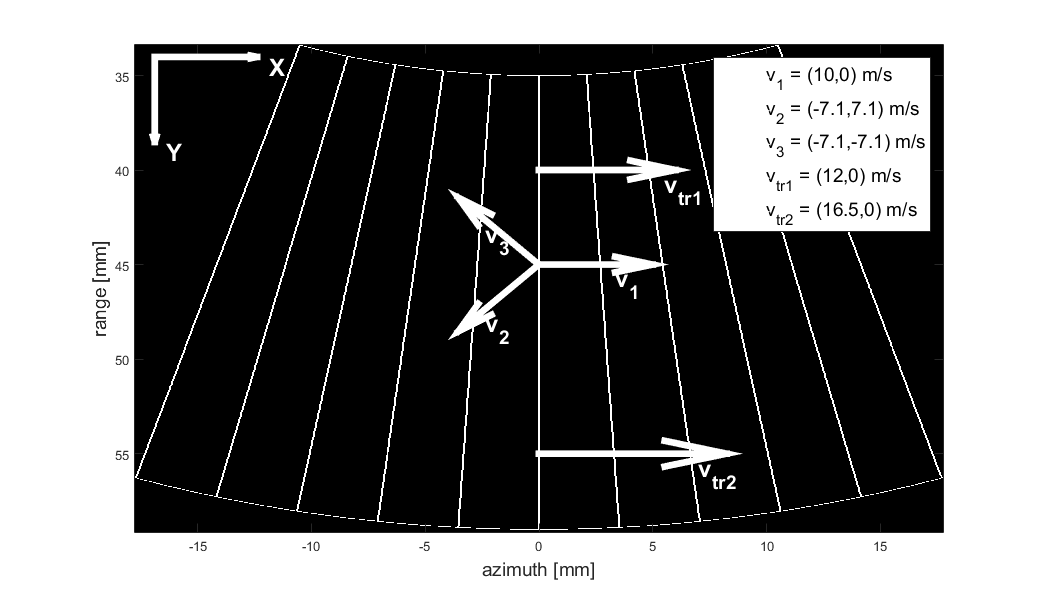
\includegraphics[width=\linewidth]{./images/results/2.1/velocities.png}
    \caption[Illustration of beamformed image with various velocities.]{Illustration of beamformed image with various velocities. The velocity vectors are at a different scale than the image azimuth and range.}
    \label{fig:velocities}
\end{figure}

If not mentioned otherwise, all beamformed images of this section are considered to be built from $b_{tr} = 65$ transmit beams and $b_{re} = 3 \cdot 65 = 195$ receive beams. The number of transmit beams corresponds to the required number of beams to guarantee no visible scalloping loss for DAS in a noiseless medium and $b_{re} = 195$ ensures no visible scalloping loss for the IAA and DAS beamformers (Table \ref{table:num_beams}).
In order to simulate perfect multiline acquisition (MLA) on reception, the images are actually created from $b_{tr} = b_{re} = 195$ beams, but the image acquisition time is still considered to be $t_{im} = 0.3 \cdot 65 / 1500 = 0.013~$s = 13 ms.
We could also have chosen $b_{re} \geq 981$ in order to ensure no visible scalloping loss for the MV beamformer as well, but 
such high beam densities are too computationally demanding for us to run all the experiments with such simulations.
Furthermore, we consider such beam densities to be too high to be realistically implementable and therefore not very interesting to analyze.

The linear motion of a scatterer point is, as explained previously, simulated with a constant shift of its position before each beam transmit and recording. With the MLA approach, the scatterer points should actually only move in between two transmit beams and remain static for receive beams constructed from the same transmit beam. With a MLA coefficient of $MLA_c = b_{re} / b_{tr} = 195 / 65 = 3$, the scatterer points should only be shifted once every three receive beams.
We have however chosen to have the scatterer point shifted in between all beams for two main reasons.
First of all, with continuous motion, the results of this section can be extended to MLA approaches with virtually any coefficient value $MLA_c$, including single-line acquisition ($MLA_c = 1$). Secondly, this thesis focuses on worst-case scenarios and continuous motion seems to us to be a bigger divergence from the beamformers' model of static points than partial motion. We do not expect the partial motion implementation to result in additional artifacts.


\subsection{Single scatterer point in a noiseless medium}
\label{sec:single_noiseless}
In this thesis, a scatterer point shape in a beamformed image is defined by the area within 3 dB of its peak gain. This section focuses on imaging a single scatterer point and analyzing the effects of motion within frames on its shape.

As initial exposure to motion within frames, let us start with a simple example. A single scatterer point $s$ is positioned at $40~$mm range and $0~$mm azimuth in a noiseless medium. In this example, $s_1$ is imaged with different lateral velocities $\boldsymbol{v}_s = (v_x, 0),~ v_x \in \{-0.6, 0, 0.6\}~$m/s.
The DAS beamformed image and steered response of $s_1$ when static are displayed in Figure \ref{fig:DAS_steered}. The problems with those plots are that the beamformed image does not clearly outline the shape of the scatterer point and the steered response plot only shows its width. Instead, we have chosen to replace both plots with a contour plot of the beamformed image with 3 color-coded gain levels (from darkest to brightest): max-100, max-10 and max-3 dB.
Figure \ref{fig:DAS_steered} can then be replaced by the DAS contour plot of Figure \ref{fig:DAS_idle}, where the white area represents the perceived shape of the scatterer point.
This contour plot representation is used as a visualization tool for the rest of this thesis.

\begin{figure}[ht]
    \centering
    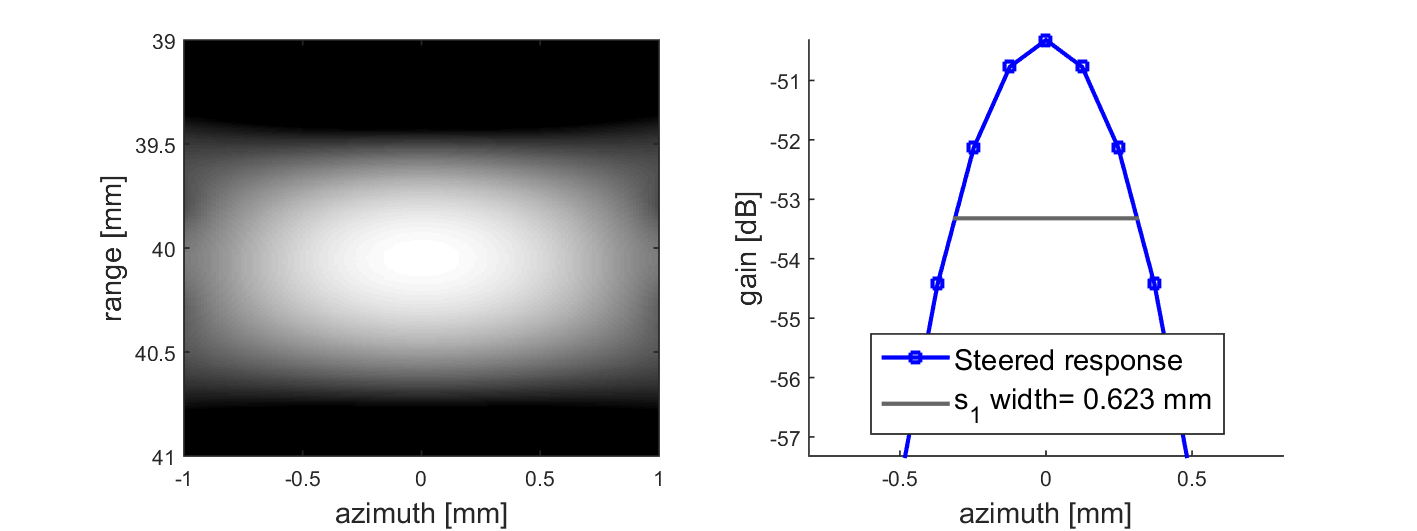
\includegraphics[width=\linewidth]{./images/results/2.1/DAS_steered2.png}
	\caption{DAS beamformed image and steered response of a static scatter point in a noiseless medium.}
	\label{fig:DAS_steered}
\end{figure}

\begin{figure}[ht]
    \centering
    \begin{subfigure}[t]{0.48\linewidth}
        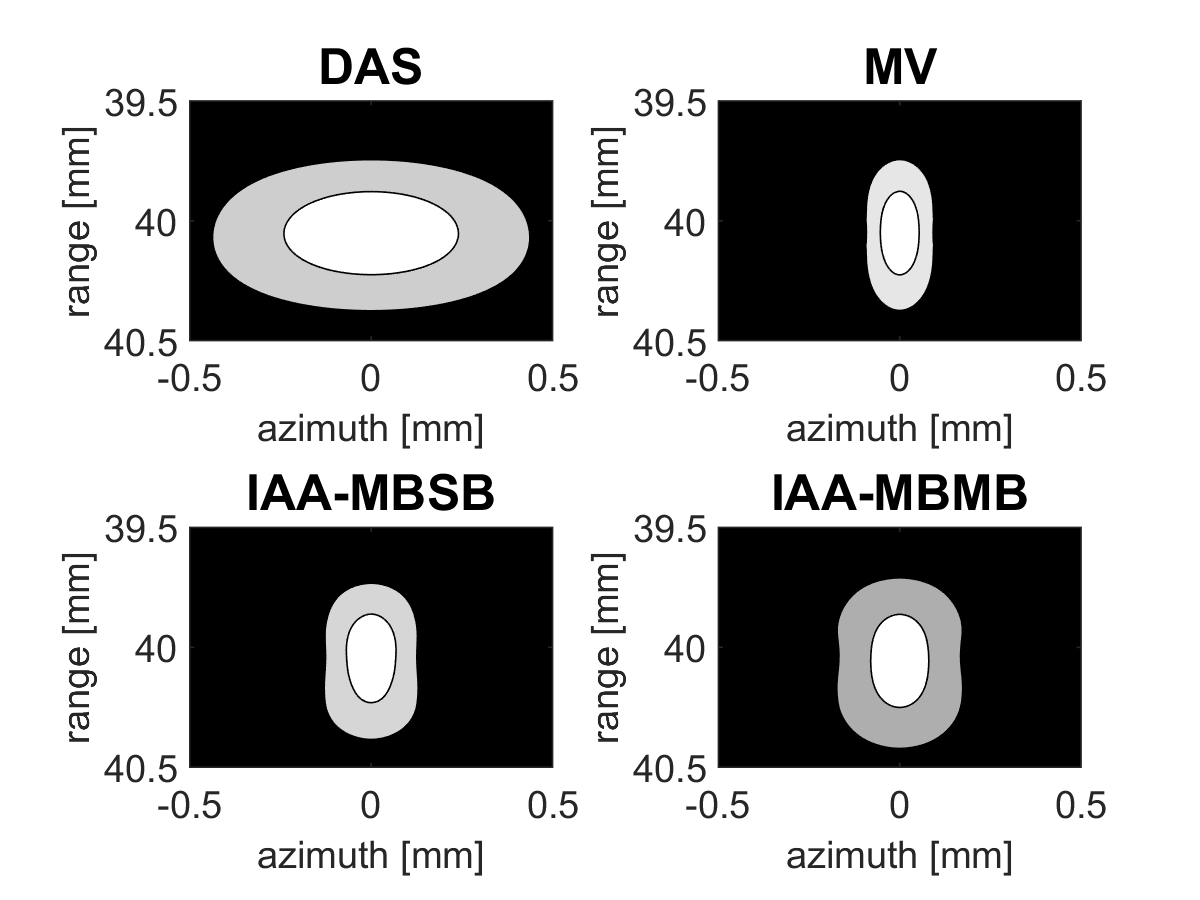
\includegraphics[width=\linewidth]{./images/results/2.1/motion_0_-06.png}
        \caption{$v_x = -0.6~$m/s.}
    \end{subfigure}
    \quad
    \begin{subfigure}[t]{0.48\linewidth}
        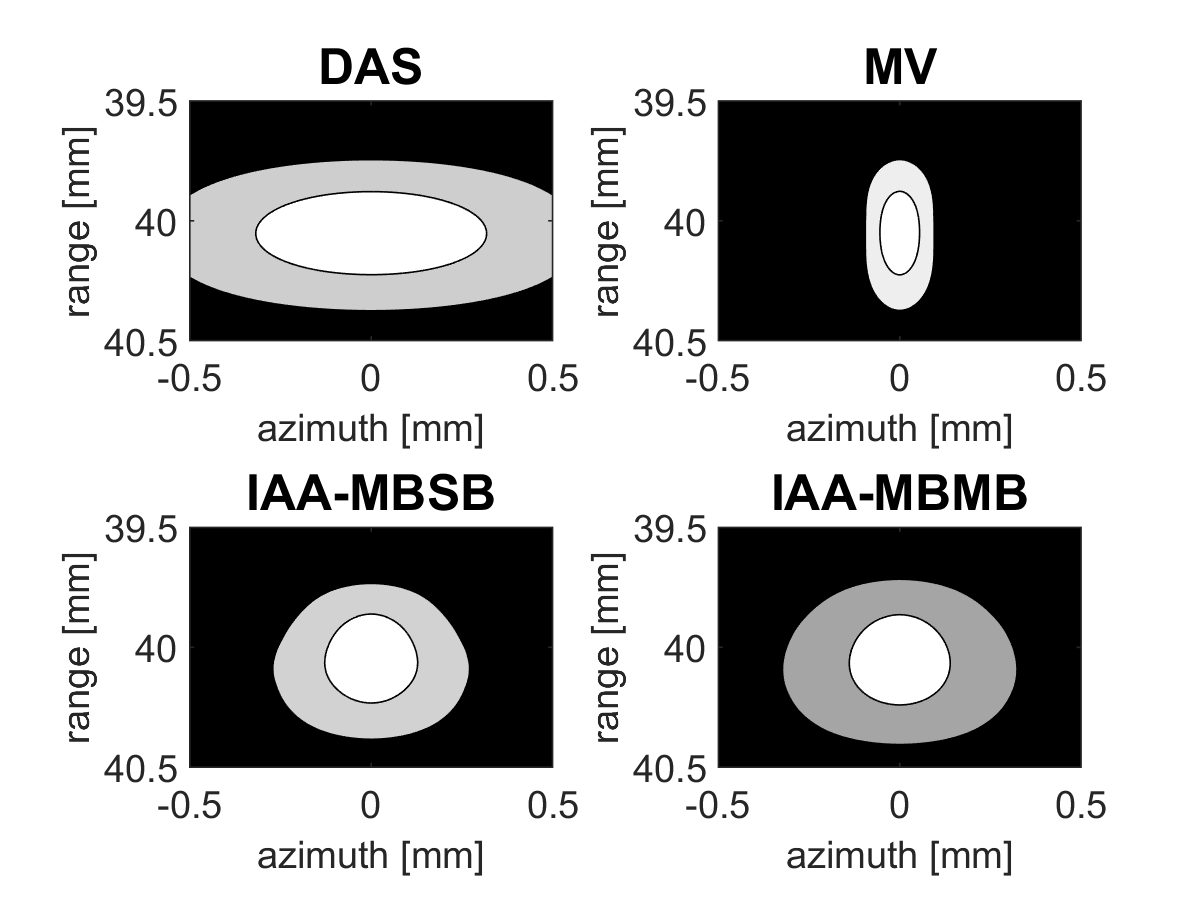
\includegraphics[width=\linewidth]{./images/results/2.1/motion_0_0.png}
        \caption{$v_x = 0~$m/s.}
        \label{fig:DAS_idle}
    \end{subfigure}
    \quad
    \begin{subfigure}[t]{0.48\linewidth}
        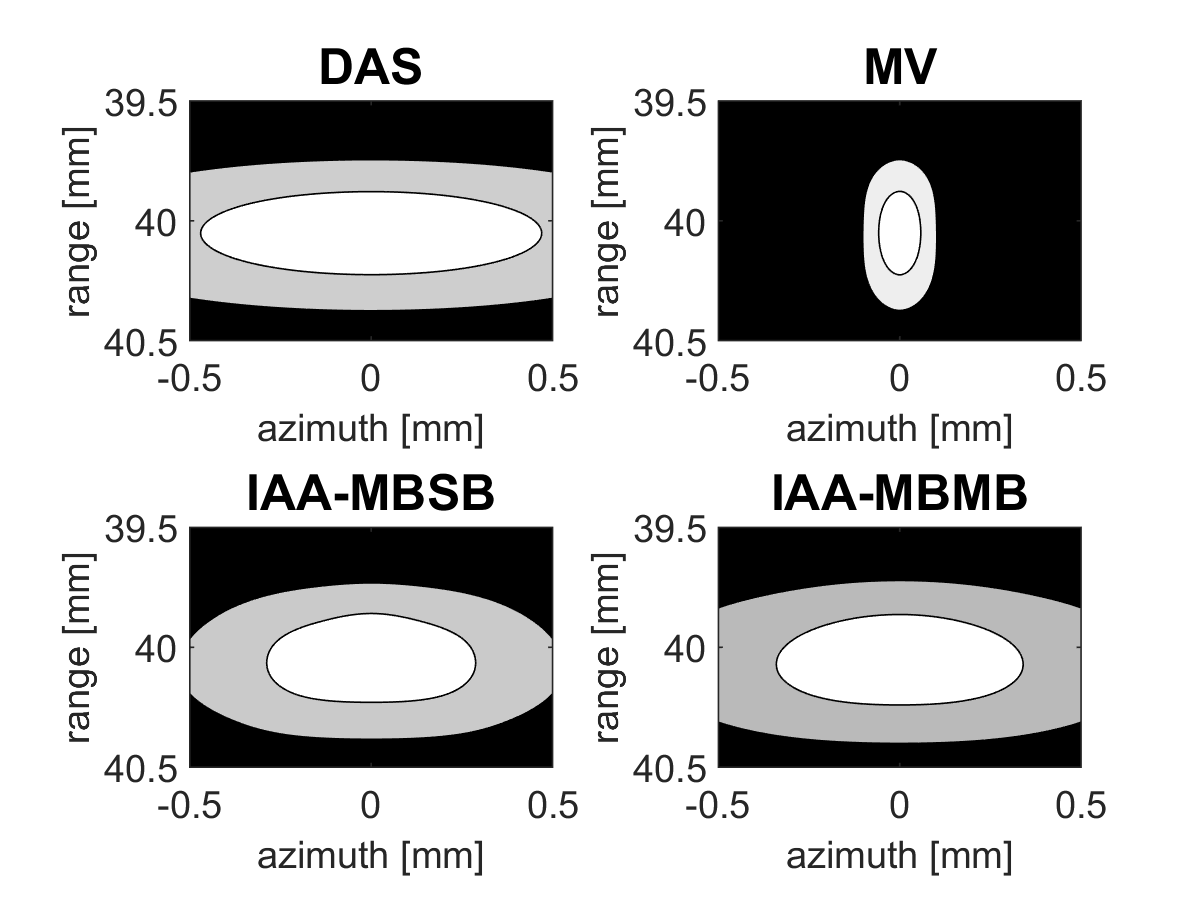
\includegraphics[width=\linewidth]{./images/results/2.1/motion_0_06.png}
        \caption{$v_x = 0.6~$m/s.}
    \end{subfigure}
	\caption{Contour plot of DAS beamformed images. Scatter point in lateral motion in a noiseless medium: $\boldsymbol{v}_s = (v_x, 0)~$m/s, $v_x \in \{-0.6, 0, 0.6\}$.}
	\label{fig:illustration_all}
\end{figure}

Figure \ref{fig:illustration_all} displays the results of the current experiment for the three different velocities $v_x \in \{-0.6, 0, 0.6\}~$m/s and all beamformers.
First of all, the beamformers obviously have different resolution capacities, which is why the shape of the scatterer point varies so much depending on the beamformer used even if static (Figure \ref{fig:DAS_idle}). The comparison of the DAS and MV beamformed images gives a good example of why the MV beamformer has historically been introduced as a high-resolution algorithm.

Compared to the static scene, the scatterer point consistently appears bigger when it is moving in the same direction as $v_{tr}$ ($v_x > 0$) and smaller when $v_x < 0$, although the size variation is hardly visible in the MV beamformed images. The MV beamformer seems much less sensitive to lateral motion than the other beamformers.
But, besides this lateral dilation or erosion of the scatterer point's shape, none of the beamformed images seem to contain visible artifacts.
It is worth mentioning that, in this section, all images are built such that the scatterer point is at $0~$mm azimuth when the center beam is transmitted, regardless of the point's velocity, which is why the center of its shape always is at $0~$mm azimuth and $40~$mm range.
That way we limit potential artifact due to differences in the scatterer point's position, including possibly visible scalloping loss for the MV beamformer.
Note that a scatterer point having a linear motion type, even at constant range, has a varying radius to the array, which means that it can potentially go in and out of the array's focus radius.

For the next experiment, multiple frames are simulated with a single scatterer point located at $40~$mm range and moving at different lateral velocities $v_x$ from -0.6 to 0.6 m/s.
For any given frame, the width of the scatterer point is estimated by the mainlobe width of the array's steered response at $40~$mm radius. For each frame, the resulting scatterer point width is displayed in Figure \ref{fig:width_vs_velocity} both as an absolute value and as a relative increase, in $\%$, compared to that of the scatterer point when static.

\begin{figure}[ht]
    \centering
    \begin{subfigure}[t]{\linewidth}
        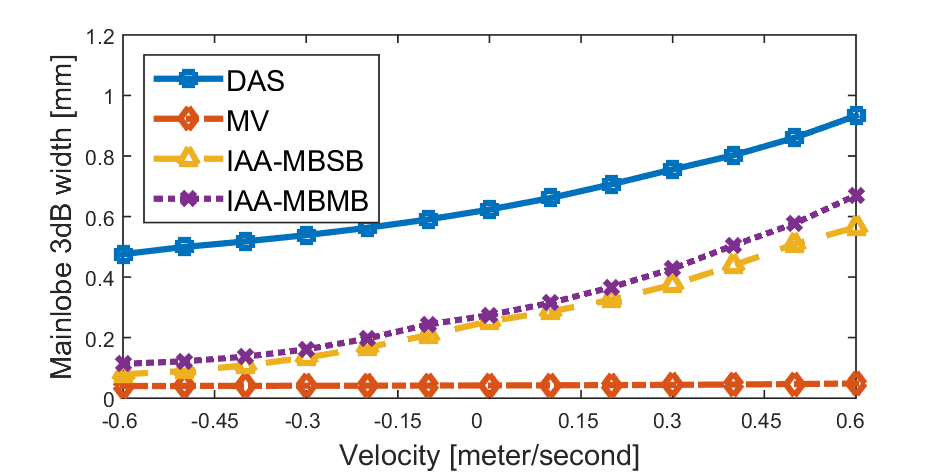
\includegraphics[width=\linewidth]{./images/results/2.1/mainlobe_width_65.png}
        \caption{Steered response mainlobe width in mm.}
        \label{fig:width_vs_velocity_a}
    \end{subfigure}
    \quad
    \begin{subfigure}[t]{\linewidth}
        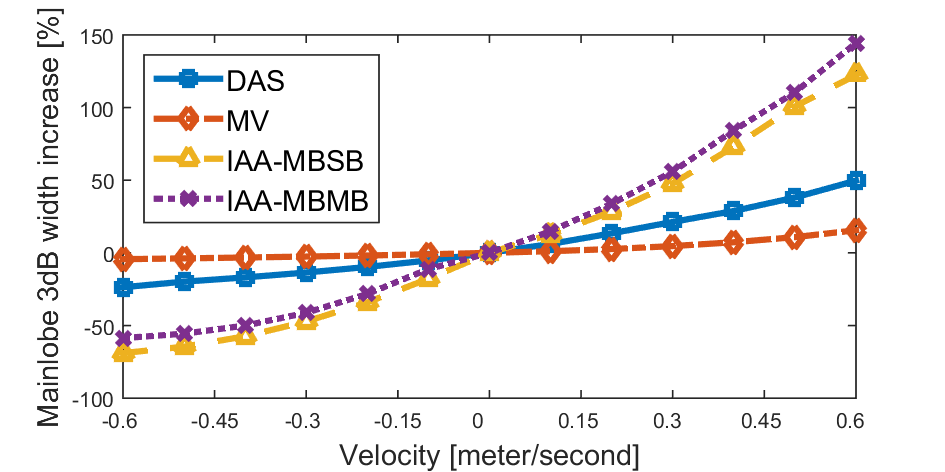
\includegraphics[width=\linewidth]{./images/results/2.1/mainlobe_width_65_rel.png}
        \caption{Steered response mainlobe width relative to that of the static scatterer point scenario.}
        \label{fig:width_vs_velocity_b}
    \end{subfigure}
	\caption{Scatter point in lateral motion in a noiseless medium: $\boldsymbol{v}_s = (v_x, 0)~$m/s, $-0.6 \leq v_x \leq 0.6$.}
	\label{fig:width_vs_velocity}
\end{figure}

As predicted in Table \ref{table:panoramic_imperfect}, the point's apparent width gets dilated with positive velocities along its motion path. Motions opposite to the beam distribution direction ($v_x < 0$) result in the point's width appearing smaller. This can be explained by the fact that the scatterer point potentially hits more transmit beams as $v_x$ increases. Following that principle, if $v_x$ increases to very high values, the apparent width of the scatterer point should decrease. The maximum apparent width should happen when $v_x$ is equal to $v_{tr}$, where $v_{tr}$ is defined by Equation (\ref{eq:vtr}). This statement can be confirmed by extending the current experiment to extreme velocities. The results with velocities $v_x \leq 3~$m/s are displayed in Figure \ref{fig:width_vs_velocity_ext_pos}. With $b_{tr} = 65$, the acquisition lateral velocity at $40~$mm radius is $v_{tr_{40}} = 1500 \cdot 40 \cdot 10^{-3} / \lfloor 65 / 2 \rfloor = 60 / 32 = 1.875~$m/s. For all beamformers, the scatterer point's width increases with its lateral velocity $v_x$ and peaks when $v_x = v_{tr}$, then decreases as $v_x$ increases beyond that. This effect is indeed not an artifact caused by a particular beamformer algorithm but by a physical limitation, even if different beamformers have different sensitivities to that effect.

\begin{figure}[ht]
    \centering
    \begin{subfigure}[t]{\linewidth}
        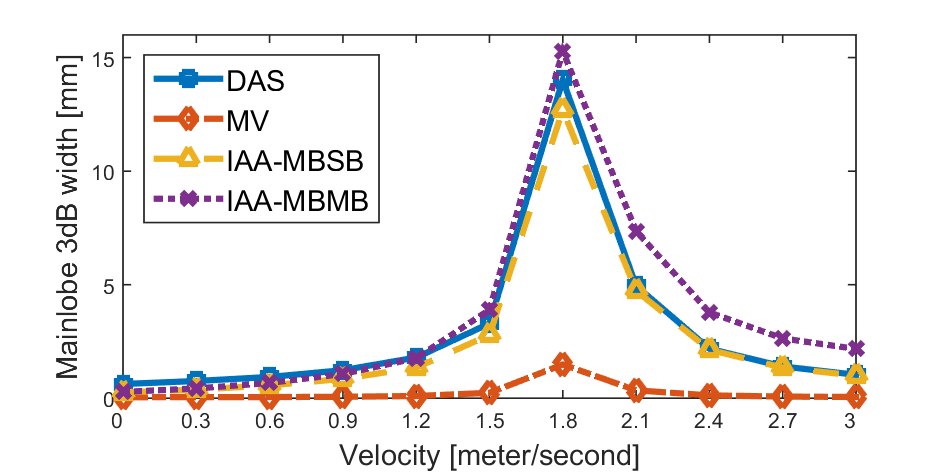
\includegraphics[width=\linewidth]{./images/results/2.1/speeds_ext_pos.png}
        \caption{$0 \leq v_x \leq 3~$m/s.}
	    \label{fig:width_vs_velocity_ext_pos}
    \end{subfigure}
    \quad
    \begin{subfigure}[t]{\linewidth}
        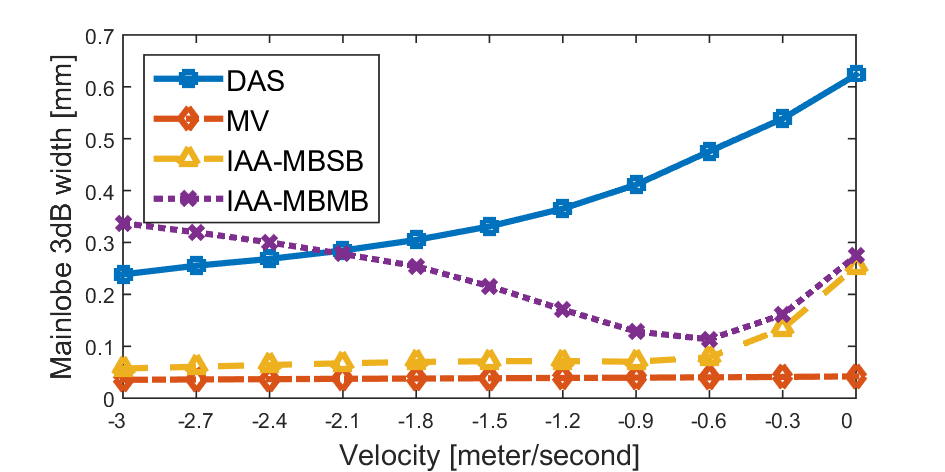
\includegraphics[width=\linewidth]{./images/results/2.1/speeds_ext_neg.png}
        \caption{$-3 \leq v_x \leq 0~$m/s.}
	    \label{fig:width_vs_velocity_ext_neg}
    \end{subfigure}
	\caption{Scatter point in lateral motion in a noiseless medium: $\boldsymbol{v}_s = (v_x, 0)~$m/s, $-3 \leq v_x \leq 3$.}
	\label{fig:width_vs_velocity_ext}
\end{figure}

In most imaging applications, one would want to avoid scenarios where $v_x$ converges towards $v_{tr}$, since the scatterer point can potentially appear much wider than it should and may result in a dramatic loss of resolution.
This imposes an upper limitation on the number of transmit beams. Such a limitation depends on how much resolution loss is considered acceptable, which depends on the application.
As an example, let us consider the limitation that any scatterer point should not move faster than 80\% of the beam distribution velocity: $v_x \leq 0.8 \cdot v_{tr}$.
Adding to that the assumption of Section \ref{sec:beams_motion} that $\boldsymbol{v}_s \leq 0.6$ m/s, the upper limit beam distribution velocity with this setup is: $v_{tr} = 0.6 / 0.8 = 0.75$ m/s. Since $v_{tr}$ is defined in Equation (\ref{eq:vtr}) as a function of the range $r$, for $b_{tr} = 65$, the upper limit of $v_{tr}$ implicitly sets a minimum range limit $r_{lim} = v_{tr} \cdot \lfloor b_{tr} / 2 \rfloor / 1500 = 0.75 \cdot 32 / 1500 = 16~$mm. This means that, in this example, resolution losses beyond what is considered acceptable might occur for range values $r < 16~$mm.

As mentioned previously, the cause of the apparent dilation or erosion of a scatterer point is a physical one, but different beamformers have different sensitivities to that effect. A quick comparison of the DAS and MV beamformers shows that the MV beamformer is much less sensitive to lateral motion, for the same beam density, both in terms of absolute mainlobe width or relative width increase. One could then speculate that, for singlebeam beamformers, their sensitivity to lateral motion is highly correlated with the mainlobe width of their receive beams.
Although we do not prove this speculation in this thesis, it seems logical that, given the same beam density, creating wider beams would result in the scatterer point hitting more of them and, consequently, lead to increased sensitivity to lateral motion.

Regardless of the veracity of this speculation, the sensitivity to lateral motion of the multibeam IAA approaches can not be solely explained from their mainlobe width. They appear indeed more sensitive to motion than their sheer mainlobe width would suggest.
The IAA beamformers are based on the sparse signal representation approach (\cite{Yardibi_nonparametric_IAA}), which means that they model static scatterer points and try to adapt that model to the recorded data.
A moving point does not fit well with this model since the different beams can potentially hold contradicting information about the presence of a scatterer point in a given direction.
When combining the receive beams into a multibeam covariance matrix estimate, the mismatch between the beams' information can cause distortions in the scatterer point's apparent shape.
We did not know how such a divergence between the expected model and the recorded data would affect the performance of the IAA beamformers.
We see from Figures \ref{fig:illustration_all} and \ref{fig:width_vs_velocity_ext} that this divergence only seems to result in loss of image resolution.
The IAA-MBSB beamformer is more sensitive than DAS in terms of relative loss of resolution, but still maintains an absolute resolution under or equal to that of the DAS.
The width of the scatterer point follows the same general pattern with the IAA-MBSB as with the singlebeam beamformers.
It increases with $v_x$, peaks at $v_x = v_{tr}$ and then decreases.

The IAA-MBMB, on the other hand, displays a different behaviour with $v_x \leq -0.6~$m/s. While, with the other beamformers, the width of the scatterer point diminishes with $v_x$ going towards $-\infty$, it appears with IAA-MBMB to grow back and even beyond its value when static.
The IAA-MBMB is also altogether more sensitive to lateral motion than IAA-MBSB and can yield results with lower resolution than DAS for relatively high velocities, both positive and negative.
Both the IAA-MBSB and IAA-MBMB beamformers suffer from this discrepancy of the imaged medium from the assumed model. However, the IAA-MBMB approach is more sensitive to this divergence since it uses the multibeam $\boldsymbol{\hat{R}}$ for the final estimate of the scatterer point amplitudes (Equation (\ref{eq:mb_output})), whereas the IAA-MBSB approach only uses the corresponding time- and phase-shifted array data for that final step (Equation (\ref{eq:sb_output})).

For the next experiment, scatterer points moving in different directions are imaged. The beamformed images are simulated in the same manner as for the previous experiment, with a single scatterer point moving in a noiseless medium. The only difference is that the scatterer point is not only assumed to move laterally ($v_x \neq 0$), but also vertically ($v_y \neq 0$). The goal of this experiment is to find out if the vertical component of a scatterer point's velocity induces additional artifacts in its apparent shape. Different scatterer point velocities $\boldsymbol{v}_s$  such that $|\boldsymbol{v}_s| = 0.6~$m/s are experimented with and the resulting beamformed images are displayed in Figure \ref{fig:linear_motion}.

The results of Figure \ref{fig:linear_motion} converge with those of Figure \ref{fig:width_vs_velocity} in the sense that motion within frames only seems to result in dilation or erosion of the scatterer point. However, it is worth noticing that the direction of dilation $\boldsymbol{d}_s = (d_x, d_y)~$m does not always correspond to the direction of motion $\boldsymbol{v}_s = (v_x, v_y)~$m/s. 
The Y component $d_y$ is always of same sign as $v_y$, but the X component is not only dependent on $v_x$, but also $v_y$ and $v_{tr}$.
Figures \ref{eq:vertical_towards} and \ref{eq:vertical_away} reveal that the scatterer point appears dilated along the X axis also with vertical linear motion ($v_x = 0$). 
Since the images are formed by sequentially transmitting beams from left to right ($v_{tr} \geq 0$), the direction of dilation has $d_x >0$ even if the scatterer point has no lateral motion. This can result in visual confusion of the direction of dilation, since the resulting scatterer point shape can look very much alike for various velocity directions.

\begin{figure}[ht]
    \centering
    \begin{subfigure}[t]{0.48\linewidth}
        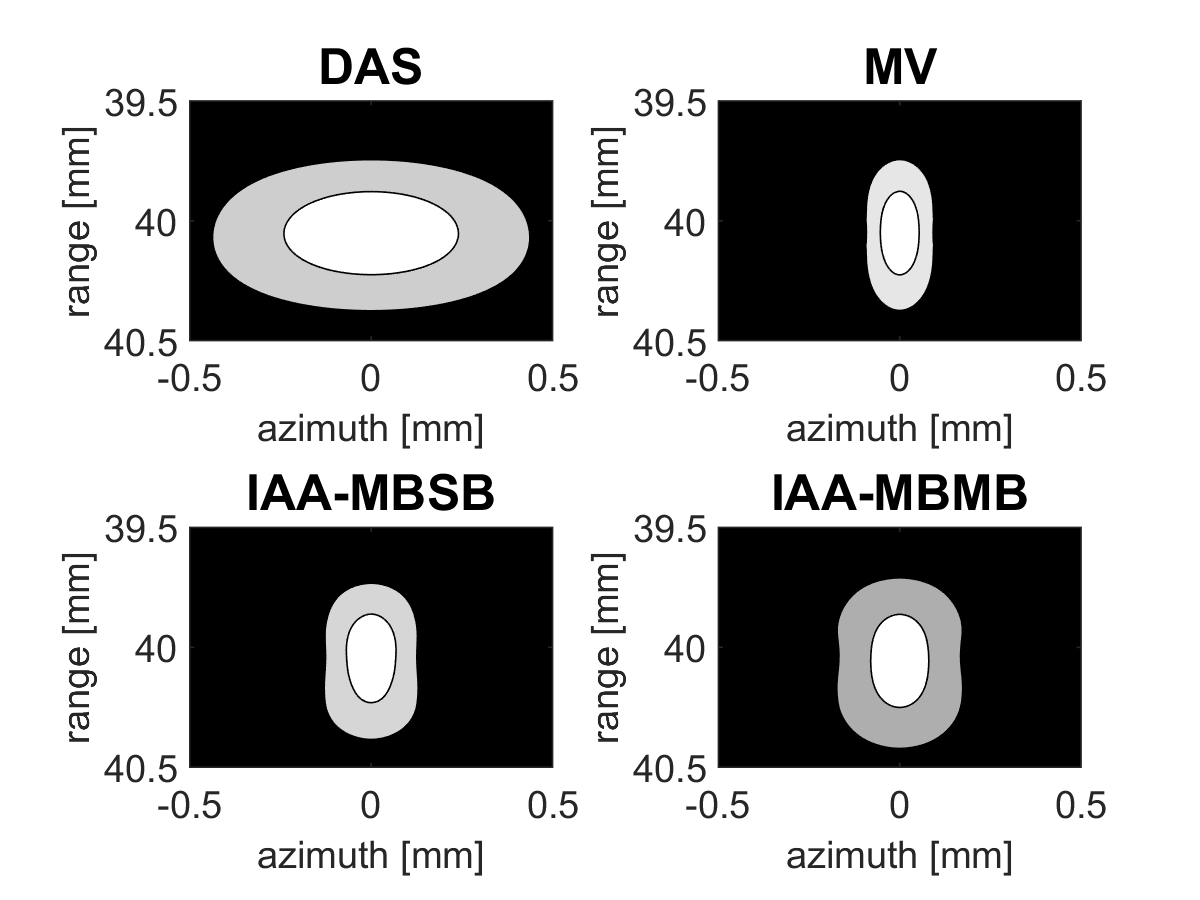
\includegraphics[width=\linewidth]{./images/results/2.1/motion_0_-06.png}
        \caption{$\boldsymbol{v}_s = (-0.6, 0)~m/s$.}
    \end{subfigure}
    \quad
    \begin{subfigure}[t]{0.48\linewidth}
        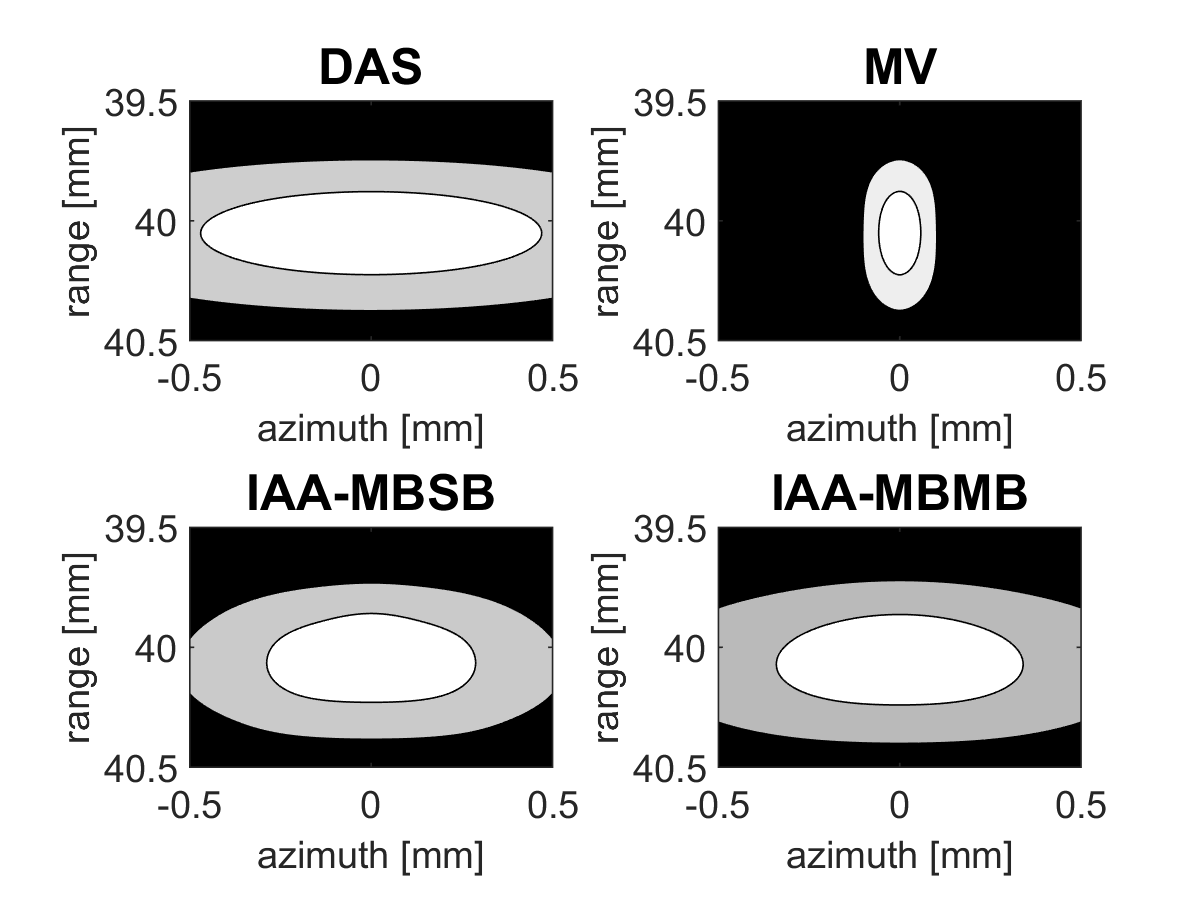
\includegraphics[width=\linewidth]{./images/results/2.1/motion_0_06.png}
        \caption{$\boldsymbol{v}_s = (0.6, 0)~m/s$.}
    \end{subfigure}
    \quad
    \begin{subfigure}[t]{0.48\linewidth}
        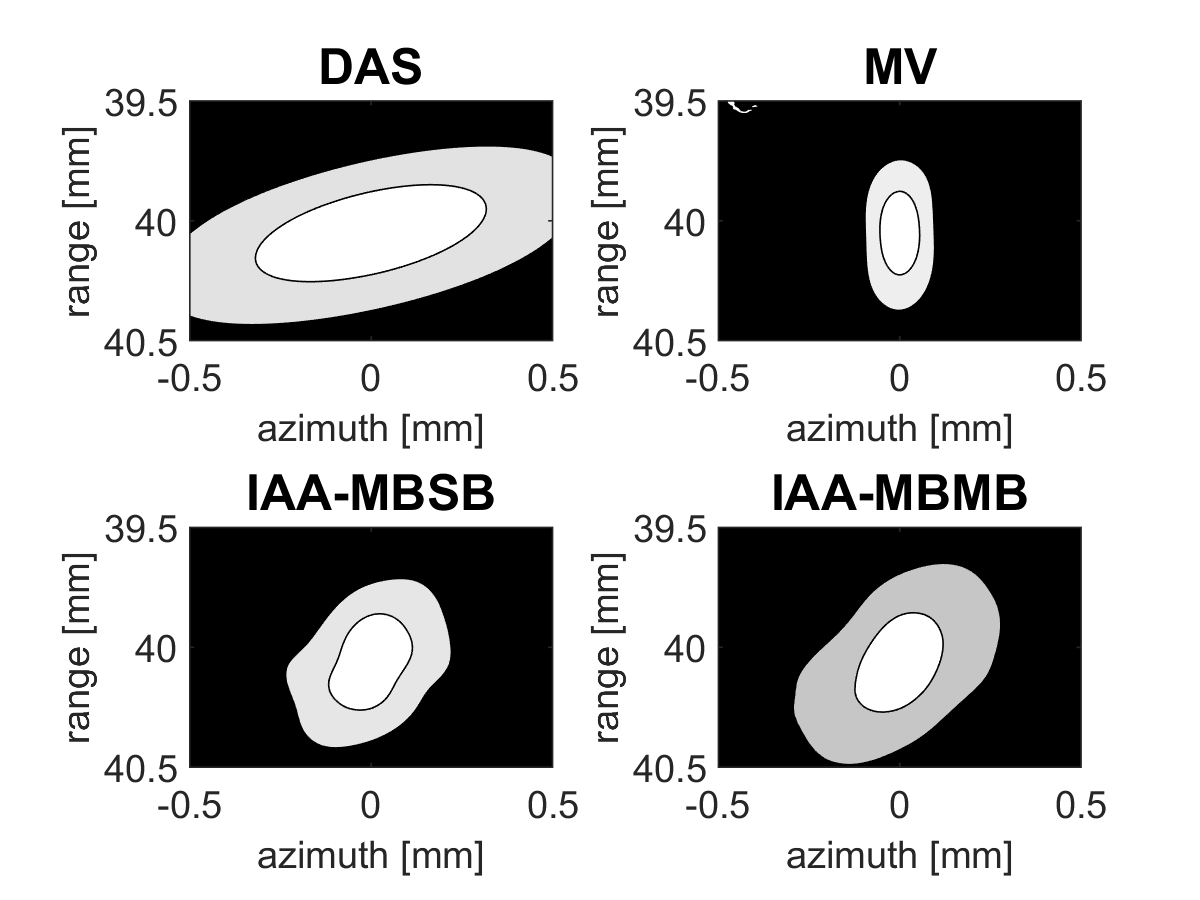
\includegraphics[width=\linewidth]{./images/results/2.1/motion_90_-06.png}
        \caption{$\boldsymbol{v}_s = (0, -0.6)~m/s$.}
        \label{eq:vertical_towards}
    \end{subfigure}
    \quad
    \begin{subfigure}[t]{0.48\linewidth}
        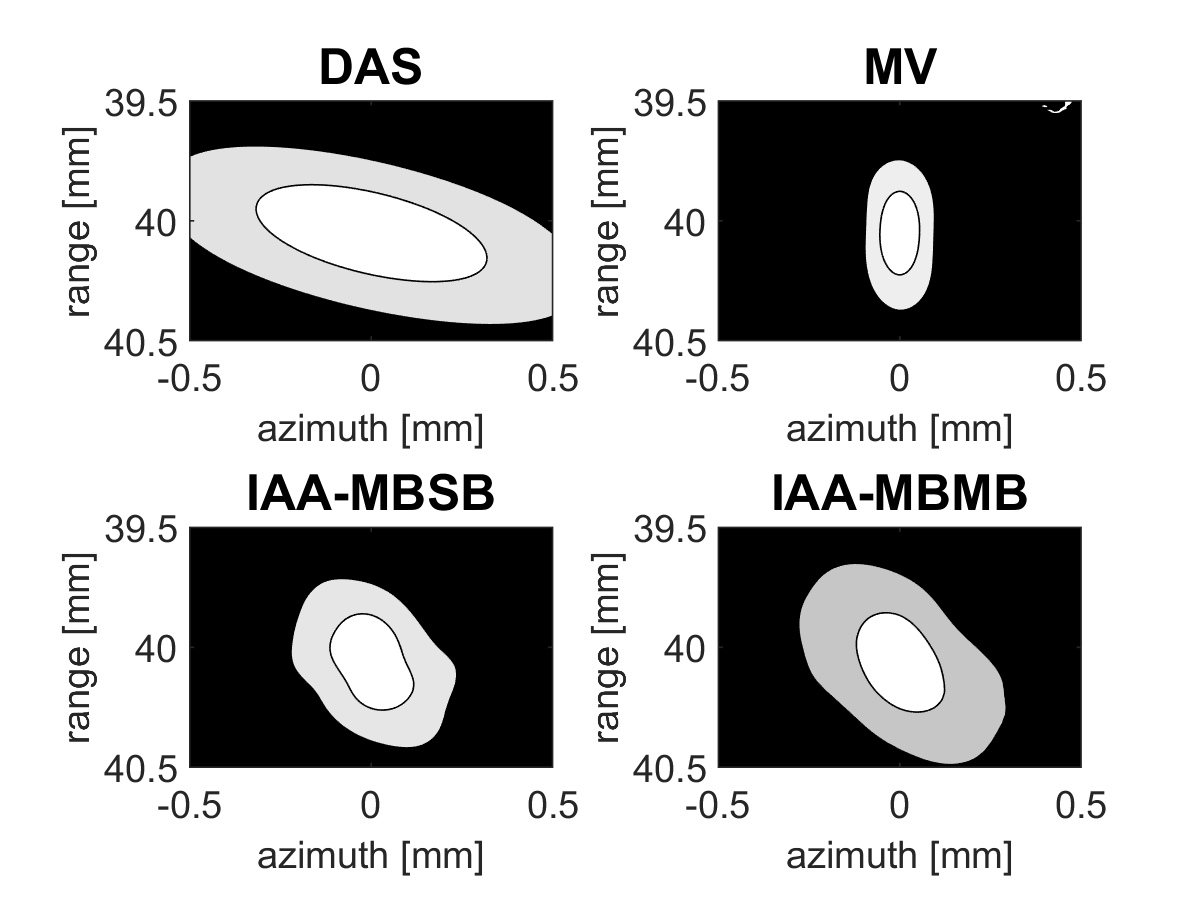
\includegraphics[width=\linewidth]{./images/results/2.1/motion_90_06.png}
        \caption{$\boldsymbol{v}_s = (0, 0.6)~m/s$.}
        \label{eq:vertical_away}
    \end{subfigure}
    \quad
    \begin{subfigure}[t]{0.48\linewidth}
        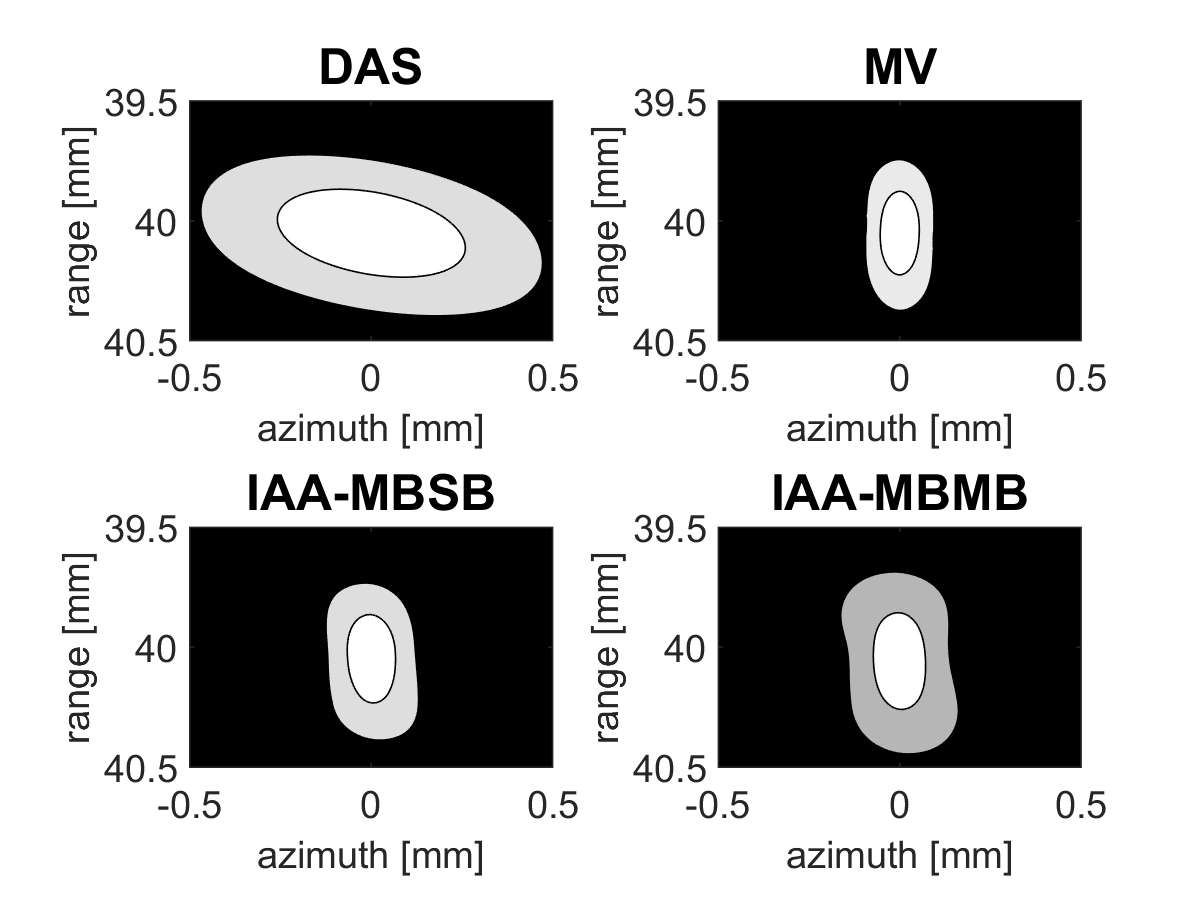
\includegraphics[width=\linewidth]{./images/results/2.1/motion_-45_-06.png}
        \caption{$\boldsymbol{v}_s = (-0.42, 0.42)~m/s$.}
    \end{subfigure}
    \quad
    \begin{subfigure}[t]{0.48\linewidth}
        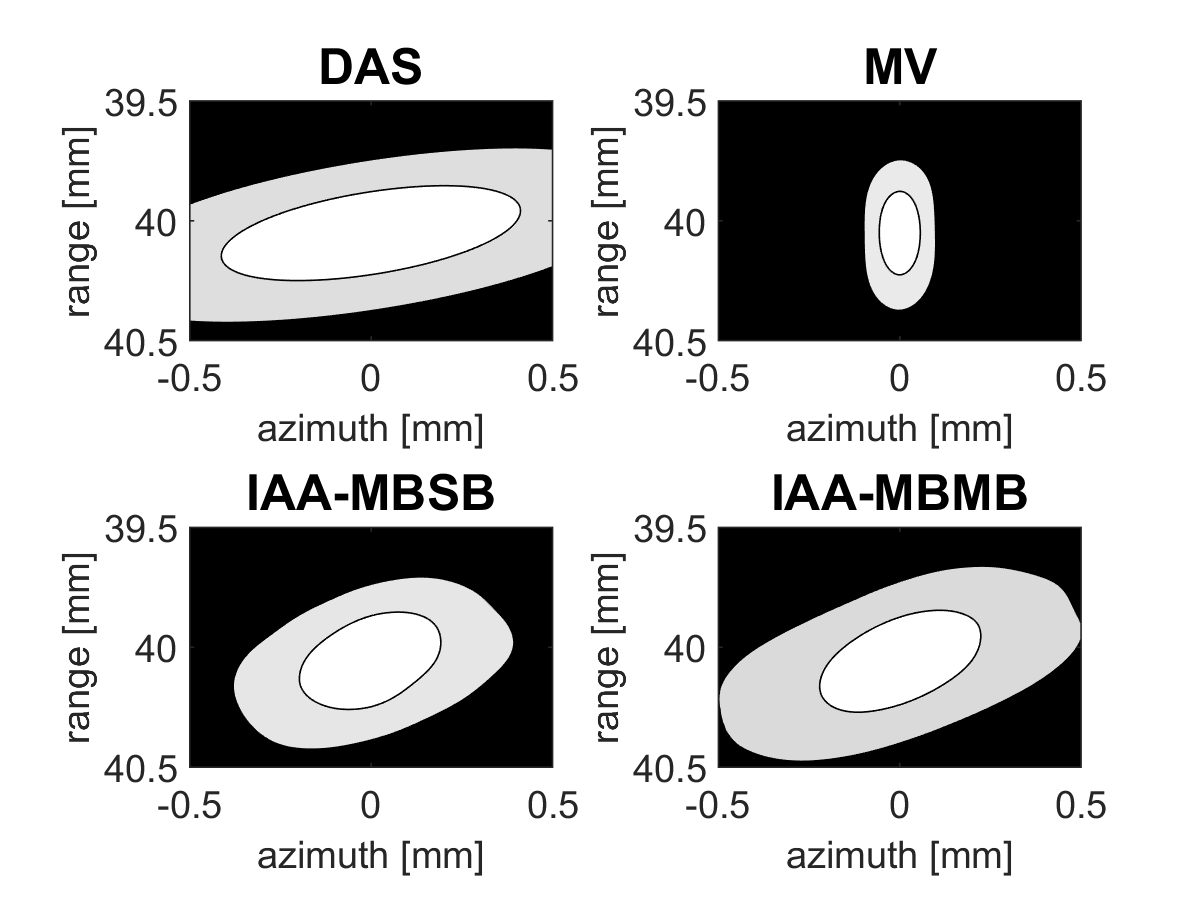
\includegraphics[width=\linewidth]{./images/results/2.1/motion_-45_06.png}
        \caption{$\boldsymbol{v}_s = (0.42, -0.42)~m/s$.}
    \end{subfigure}
    \quad
    \begin{subfigure}[t]{0.48\linewidth}
        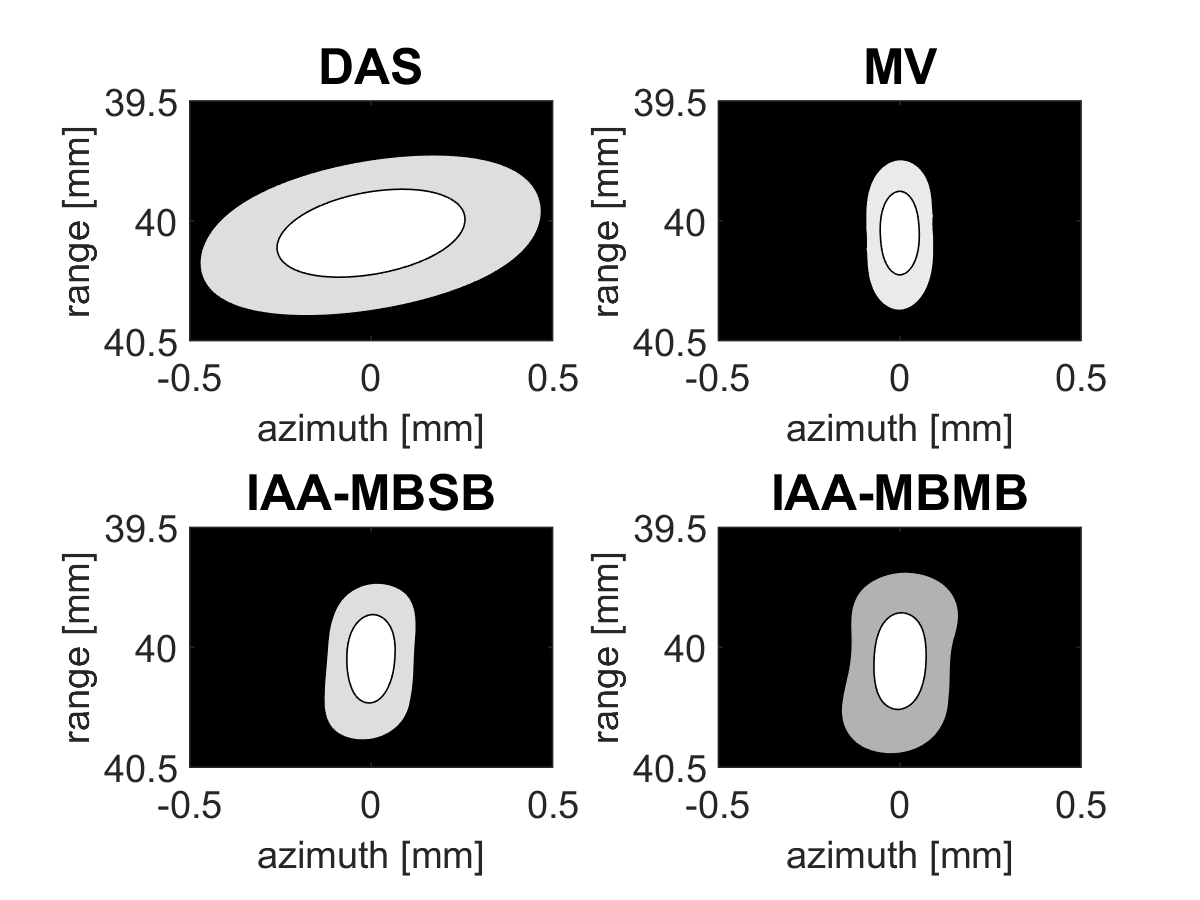
\includegraphics[width=\linewidth]{./images/results/2.1/motion_45_-06.png}
        \caption{$\boldsymbol{v}_s = (-0.42, -0.42)~m/s$.}
    \end{subfigure}
    \quad
    \begin{subfigure}[t]{0.48\linewidth}
        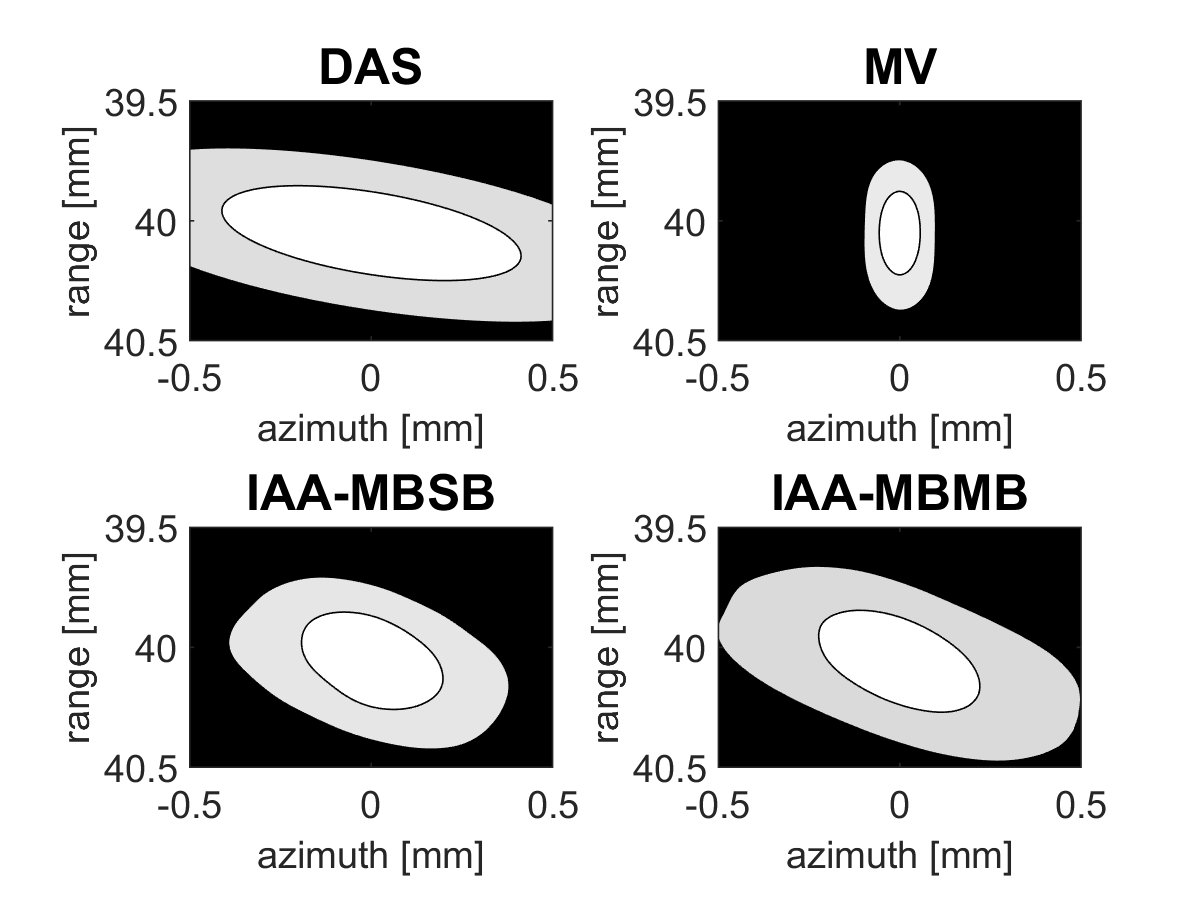
\includegraphics[width=\linewidth]{./images/results/2.1/motion_45_06.png}
        \caption{$\boldsymbol{v}_s = (0.42, 0.42)~m/s$.}
    \end{subfigure}
	\caption[A single scatterer point in various linear motions $\boldsymbol{v}_s$ with $|\boldsymbol{v}_s|=0.6~m/s$ in a noiseless medium.]{A single scatterer point in various linear motions $\boldsymbol{v}_s$ with $|\boldsymbol{v}_s|=0.6~m/s$ in a noiseless medium. Contour plot levels: max-100, max-10 and max-3 dB.}
	\label{fig:linear_motion}
\end{figure}


\clearpage
\subsection{Closely separated points in a noiseless medium}
\label{sec:twopoints_noiseless}
Section \ref{sec:spatial_smoothing} explored the issues with the presence of coherent signals in a recorded wavefield. Adaptive beamformers such as MV assume signals reflected by different scatterer points to be totally uncorrelated. Since active beamforming systems are by definition transmitting signals and recording their echoes from elements in the imaged medium, those echoes are by nature correlated.
This deviation from the model can induce apparent signal cancellation and result in lower SNR of the signals backscattered by the scatterer points in the imaged medium. The MV beamformer used in this thesis actively uses the spatial smoothing robustification method (Section \ref{sec:spatial_smoothing}) to decorrelate as much as possible the scatterer point echoes and reduce the signal cancellation effect.

The IAA approaches do not use spatial smoothing, since they are both based on the sparse signal representation and the multibeam covariance matrix estimate approaches.
As mentioned in Section \ref{sec:multibeam}, the multibeam approach can be used as an alternative method to spatial averaging to partially decorrelate spatially different signals.
Furthermore, due to the sparse signal representation, when fitting the recorded data into the covariance matrix model, the data from two closely-separated scatterer points does not match with any potential single point in the model.
For those reasons, spatial averaging is deemed not necessary for the IAA approaches.

Closely-separated scatterer points are a deviation from the expected model, not due to their proximity, since the model expects closely-separated points, but due to the high coherence of their respective backscattered signals.
The spatial averaging approach (Section \ref{sec:spatial_smoothing}) is used for the DAS and MV beamformers to decorrelate the backscattered signals. Since the length of the subarrays is typically taken as a user parameter, we can expect this approach to yield sub-optimal performances.
The IAA beamformers are able to decorrelate recorded signals without spatial averaging or required user parameter.
We therefore expect the IAA beamformers to globally yield more optimal corrections for signal coherence than the beamformers using spatial averaging.

However, we do not know how two closely-separated points in motion would affect the performances of the IAA beamformers.
We saw in Section \ref{sec:single_noiseless} that motion of a single scatterer point may result in shape distortion and resolution loss.
But the presence of motion with coherent signals might become too much of a deviation from the expected model for the IAA beamformers to correctly handle it.

In this section as well as the previous one, all beamformed images are considered to be built from $b_{tr} = 65$ transmit beams and $b_{re} = 3 \cdot 65 = 195$ receive beams by simulating perfect parallel receive beamforming. The beamformed images are also displayed as contour plots in order to outline the apparent shape of the scatterer points.
As defined in Section \ref{sec:aperture_smoothing}, two points are considered \textit{resolved} only if the minima between their peaks is of lower or equal amplitude than the lowest peak gain minus $3~$dB.
In the contour plots, the scatterer points are resolved only if their shape, delimited by the white colored layer, do not intersect.

Let us first start with static scatterer points. Two scatterer points $s_1$ and $s_2$ are simulated in a noiseless medium at $40~$mm range and respectively 0 and $0.75~$mm azimuth (or 0 and $1.07^\circ$).
With $b_{tr} = 65$, the distance between two transmit beams at $40~$mm range is $0.375~$mm. The scatterer points are therefore both located on a transmit beam trajectory and are separated by a transmit beam exactly in between them.
Since both points are static and on a transmit beam trajectory, they are not subject to scalloping loss.
The resulting beamformed images are displayed in Figure \ref{fig:two_points_static}.
In this case, none of the beamformers are able to resolve the two scatterer points, although the MV beamformer is very close to achieving it. The two points are spatially too correlated, or in other words too close to each other, for the beamformers to resolve them.

Before adding motion into the imaged scene, it is worth having a short reflection on the image acquisition sequence. In this thesis, an image is formed by sequentially transmitting and recording beams with their focus point shifted from negative azimuth to positive azimuth, or in other words, towards positive X (Figure \ref{fig:velocities}). Imagining that a scatterer point $s_1$ located at position $(x_1, y_1)$ is illuminated at time $t_1$, then any point $s_2$ located at position $(x_2, y_2)$, such that $x_2 > x_1$ is illuminated at time $t_2 \geq t_1$. If the scatterer points are not illuminated by the same transmit beam, then $t_2 > t_1$.
Let the true distance between $s_1$ and $s_2$ be $\delta x = x_2 - x1$ and the distance perceived by the beamformer be $\delta x_{BF}$.
Let us further assume that both $s_1$ and $s_2$ are moving at the same lateral velocity $v_x$.
Then the true distance $\delta x$ is constant regardless of $v_x$, but the perceived distance $\delta x_{BF}$ can vary depending on $\delta x$, $v_x$ and $\delta_t = t_2 - t_1$.
Based on those reflections, one could predict that lateral motion $v_x > 0$ may help to resolve closely separated scatterer points, since their apparent relative distance $\delta x_{BF}$ might increase. At the opposite, a lateral motion $v_x < 0$ may make it harder to resolve $s_1$ and $s_2$. 


\begin{figure}[ht]
    \centering
    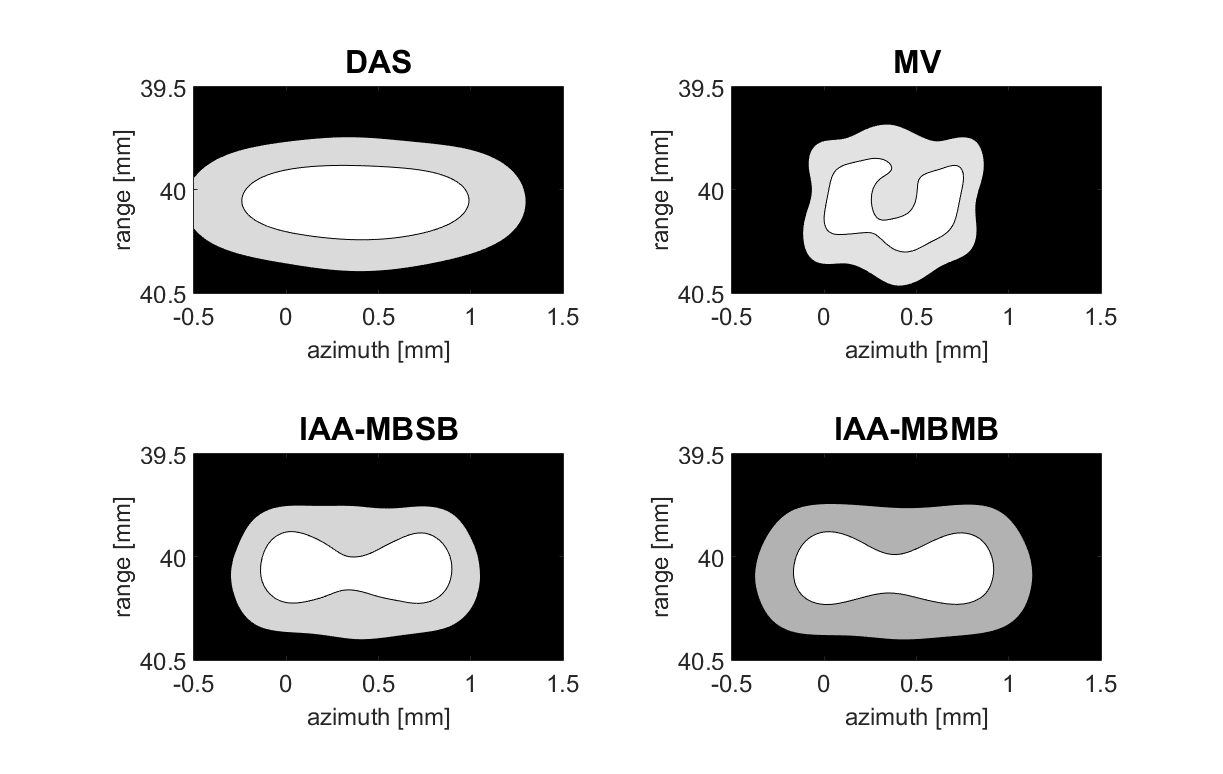
\includegraphics[width=\linewidth]{./images/results/2.2/motion_0_0.png}
    \caption[Contour plot of beamformed image with two closely-separated scatterer points in a noiseless medium.]{Contour plot of beamformed image with two closely-separated scatterer points in a noiseless medium. Color levels are: max-100, max-10 and max-3 dB.}
    \label{fig:two_points_static}
\end{figure}

Moving past static scatter points, the experiments of Section \ref{sec:single_noiseless} are reproduced with the following scenario.  Different images are simulated with the scatterer points moving in different directions at $0.6~$m/s in a noiseless medium.
In Section \ref{sec:single_noiseless}, the scatterer point was guaranteed to hit the center beam regardless of its velocity. In this section, this guarantee still holds for $s_1$, but not for $s_2$. If $s_2$ has a higher lateral velocity $v_x$ than that of the image acquisition, $v_{tr}$ as defined in Equation (\ref{eq:vtr}), it may even exit the image sector before being illuminated and would then not be detected. In our experiments, the number of transmit beams is set to $b_{tr} = 65$, which means that the image acquisition lateral velocity at $40~$mm range, defined in Equation (\ref{eq:vtr}), is $v_{tr} = 1500 \cdot 40 \cdot 10^{-3} / \lfloor b_{tr} / 2 \rfloor = 60 / 32 = 1.875~$m/s. Since the scatterer points lateral velocity $v_x \leq 0.6~$m/s, both points are guaranteed to be illuminated.
However, since $s_2$ is not guaranteed to perfectly hit a transmit beam trajectory, scalloping loss can occur. With $b_{re} = 195$ receive beams and perfect MLA, the scalloping loss is kept below the visibility threshold ($1~$dB) for the DAS, IAA-MBSB and IAA-MBMB beamformers. The effects of scalloping loss might be visible in the MV beamformed images.

The beamformed images resulting from this experiment are displayed in Figure \ref{fig:linear_motion_double} as contour plots similar to those of Figure \ref{fig:linear_motion}.
It may seem logical that introducing motion $v_x < 0$, opposite to the image acquisition direction, can add difficulties to resolve the two points, since their apparent distance $\delta x_{BF}$ decreases with $v_x$. One could then hope that the inverse is true as well, with $v_x > 0$ inducing an increased apparent distance and therefore increased chance of resolving $s_1$ and $s_2$. 
These assumptions seem to hold for the MV beamformer, but not for the IAA approaches. This can be explained by the fact that our MV beamformer is based on the single-beam covariance matrix estimation approach, whereas the IAA beamformers are based on the multibeam covariance matrix estimation (Section \ref{sec:multibeam}).
For single-beam beamformers, let us assume that the scatterer points are located in the direction matching that of the nearest beam. This assumption is technically false and a simplification of reality, but not that far from it for velocities $v_x$ well under $v_{tr}$. The first scatterer point is then always paired with the array's center beam ($\theta = 0$). If $s_2$ is paired with beam $n$, where $n=0$ is the center transmit beam, then its apparent distance to $s_1$ is $n \cdot d_B$. Lateral motion may then affect which beam $s_2$ is paired with and thus influence on the points' apparent distance.
This tendency is also true for the DAS beamformer, since it is also a single-beam beamformer. However, due to its poor resolution capacity, the DAS is not able to resolve the two scatterer points in any of the scenes of Figure \ref{fig:linear_motion_double}.

For multibeam beamformers, each beamformed image cell is built from multiple beams, so the scatterer points can not be paired with a single beam. 
If the scatterer point are moving, the beams hold different information about their location. As seen in Section \ref{sec:single_noiseless}, the more $v_x$ converges towards $v_{tr}$, the more beams are likely to illuminate the scatterer point. This divergence in the scatterer points apparent location can result in loss of resolvability.
For velocities in opposite direction ($v_x < 0$), fewer beams contain information about the same scatterer point, which means that the data is more likely to correspond to the expected model of static scatterer points.
Note that extreme velocities ($v_x < -1.2~$m/s) may cause mismatch with the expected model, since a point detected by a beam might not be detected by the neighboring beams, which might confuse the beamformer (Figure \ref{fig:width_vs_velocity_ext_neg}).

The multibeam beamformers are therefore more sensitive to positive lateral motion ($v_x > 0$) than the single-beam ones, but more robust to negative lateral motion ($v_x < 0$), at least to some extent.
The resolvability performances of the IAA approaches are, for $-0.6 \leq \boldsymbol{v}_s \leq 0.6~$m/s, at best better than MV and at worst similar to DAS.
The vertical component $v_y$ is less of a disturbance to the resolvability of the points than $v_x$. In fact, any vertical velocity, negative or positive, helps to differentiate the two points.
Figure \ref{fig:linear_motion_double} shows the same confusion of dilation direction than Figure \ref{fig:linear_motion}, where the direction of dilation $\boldsymbol{d}_s$ does not always point in the same direction as the scatterer point velocity vector $\boldsymbol{v}_s$.

\begin{figure}[ht]
    \centering
    \begin{subfigure}[t]{0.48\linewidth}
        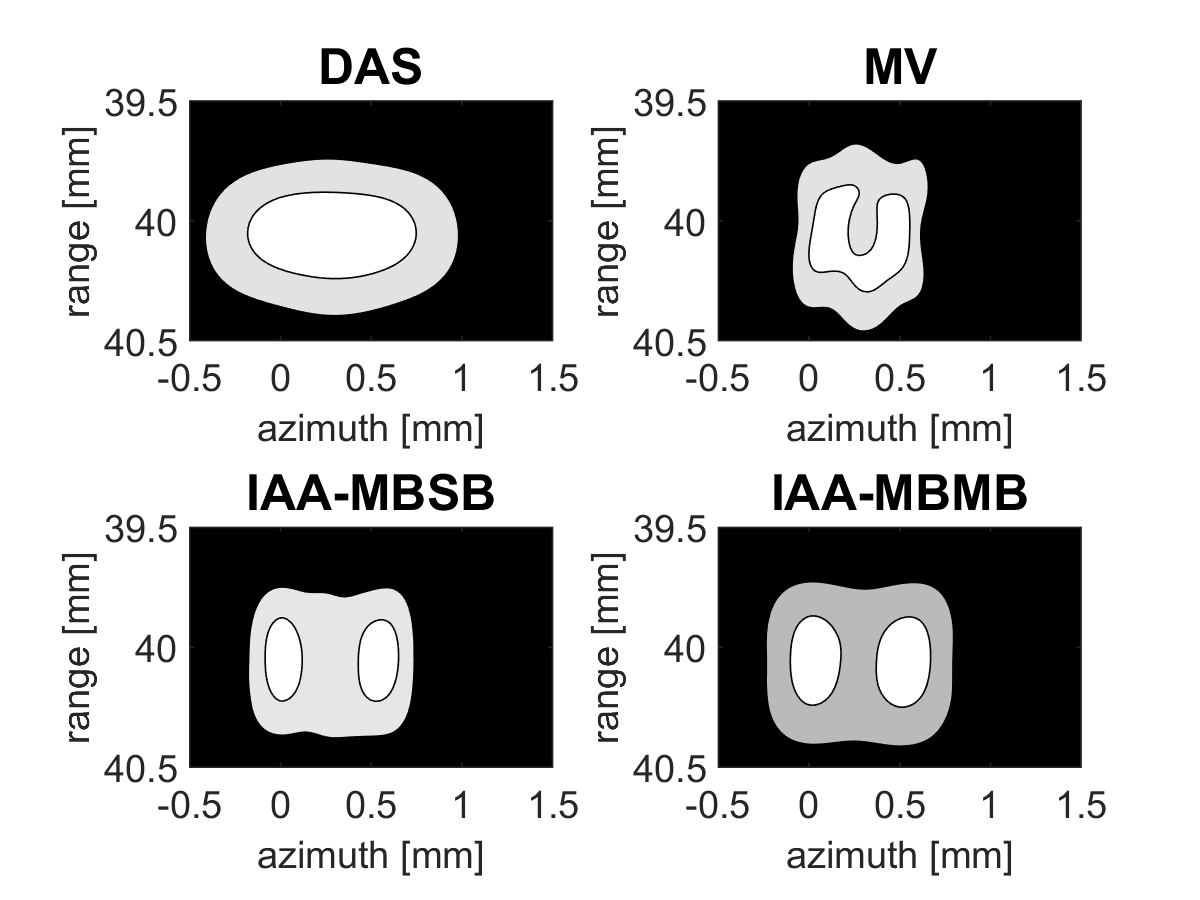
\includegraphics[width=\linewidth]{./images/results/2.2/motion_0_-06.png}
        \caption{$\boldsymbol{v}_s = (-0.6, 0)~$m/s.}
    \end{subfigure}
    \quad
    \begin{subfigure}[t]{0.48\linewidth}
        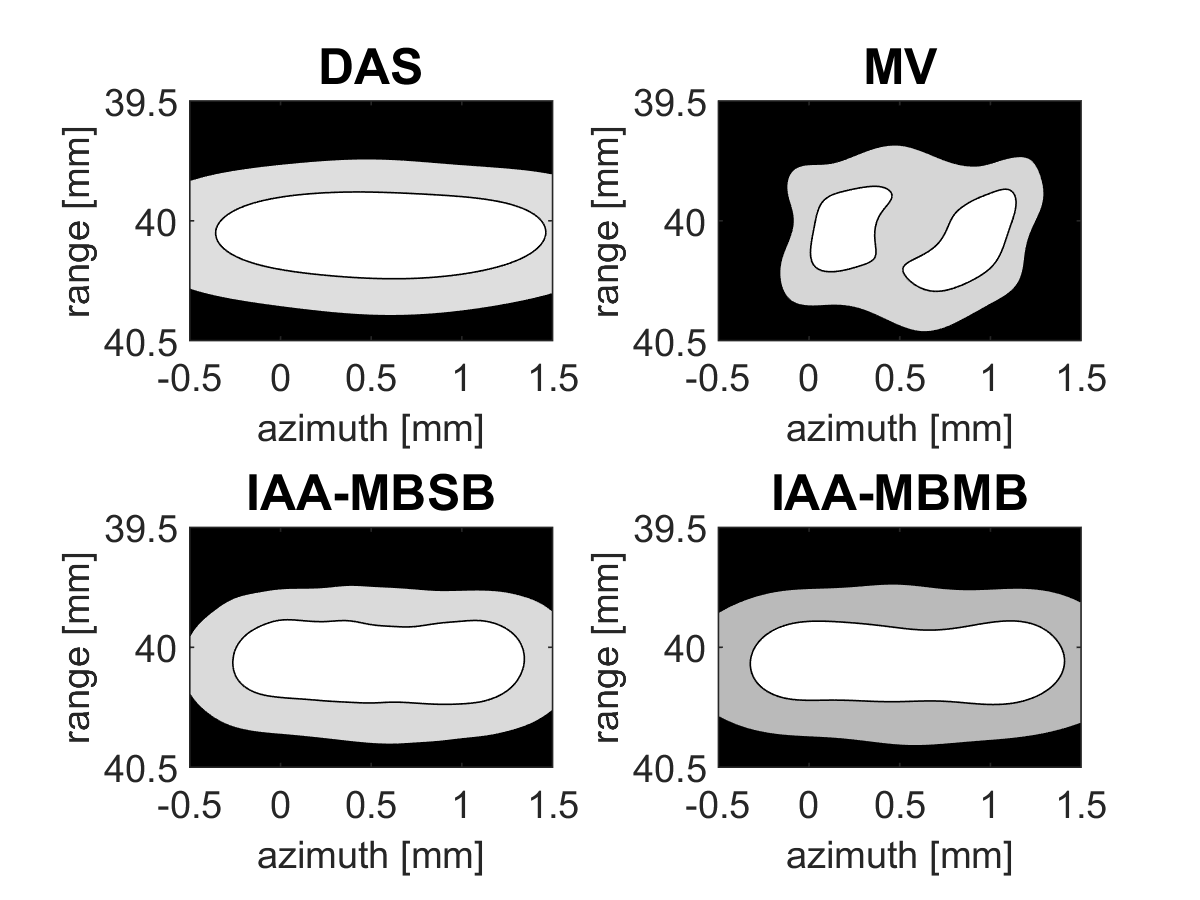
\includegraphics[width=\linewidth]{./images/results/2.2/motion_0_06.png}
        \caption{$\boldsymbol{v}_s = (0.6, 0)~$m/s.}
        \label{fig:double_lateral}
    \end{subfigure}
    \quad
    \begin{subfigure}[t]{0.48\linewidth}
        \includegraphics[width=\linewidth]{./images/results/2.2/motion_90_-06.png}
        \caption{$\boldsymbol{v}_s = (0, -0.6)~$m/s.}
    \end{subfigure}
    \quad
    \begin{subfigure}[t]{0.48\linewidth}
        \includegraphics[width=\linewidth]{./images/results/2.2/motion_90_06.png}
        \caption{$\boldsymbol{v}_s = (0, 0.6)~$m/s.}
    \end{subfigure}
    \quad
    \begin{subfigure}[t]{0.48\linewidth}
        \includegraphics[width=\linewidth]{./images/results/2.2/motion_-45_-06.png}
        \caption{$\boldsymbol{v}_s = (-0.42, 0.42)~$m/s.}
    \end{subfigure}
    \quad
    \begin{subfigure}[t]{0.48\linewidth}
        \includegraphics[width=\linewidth]{./images/results/2.2/motion_-45_06.png}
        \caption{$\boldsymbol{v}_s = (0.42, -0.42)~$m/s.}
    \end{subfigure}
    \quad
    \begin{subfigure}[t]{0.48\linewidth}
        \includegraphics[width=\linewidth]{./images/results/2.2/motion_45_-06.png}
        \caption{$\boldsymbol{v}_s = (-0.42, -0.42)~$m/s.}
    \end{subfigure}
    \quad
    \begin{subfigure}[t]{0.48\linewidth}
        \includegraphics[width=\linewidth]{./images/results/2.2/motion_45_06.png}
        \caption{$\boldsymbol{v}_s = (0.42, 0.42)~$m/s.}
    \end{subfigure}
	\caption[Two scatterer points, initially $0.75~$mm apart, in various linear motions $\boldsymbol{v}_s$ with $|\boldsymbol{v}_s|=0.6~$m/s in a noiseless medium.]{Two scatterer points, initially $0.75~$mm apart, in various linear motions $\boldsymbol{v}_s$ with $|\boldsymbol{v}_s|=0.6~$m/s in a noiseless medium. Contour plot levels: max-100, max-10 and max-3 dB.}
	\label{fig:linear_motion_double}
\end{figure}

    %\section{Improvement and robustification approaches}
\label{sec:res_improvement}
The results of Section \ref{sec:res_frames_motion} show the effects of scalloping loss can be attenuated by increasing the density of transmit beams. Although this method arguably is one of the most reliable way to reduce scalloping loss, it has several drawbacks. An increase in beams transmissions obviously results in longer image acquisition and processing time. This directly impacts the image frame rate (Table \ref{table:max_frame}). Additionally, Section \ref{sec:res_beams_motion} showed that this increased image acquisition time can result in loss of resolution with scatterer points moving in the medium.
Section \ref{sec:res_beams_motion} analyzed the effects of motion in the imaged medium during an image acquisition. Scatterer points motion can result in blur or distortion of their shape. The intensity of such distortions is dependent on the scatterer points velocity vector $\boldsymbol{v}_s$ relative to the one of the transmit beam distribution $\boldsymbol{v}_{tr}$.
The level of distortion, and therefore loss of resolution, intensifies as $\boldsymbol{v}_s$ converges towards $\boldsymbol{v}_{tr}$. This tendency is gives one more limitation to the increase of transmit beams.
Section \ref{sec:improvement} suggested several alternative approaches to reducing scalloping loss.

The first of these suggestions is to reduce the length of the transducers array. This length choice gives a trade-off between image resolution and scalloping loss magnitude. Figure \ref{fig:length_array} illustrates this statement by comparing two different array sizes for beam transmission. Besides the number of transducers used for beam transmission, all other parameters are common to both figures, including the size of the array for signal recording (96 elements).
In Figure \ref{fig:length_192}, scalloping loss is visible, but the two scatterer points are resolved. In Figure \ref{fig:length_24}, the smaller transmit array is not subject to visible, meaning higher than $1~dB$, scalloping loss. It is however unable to resolve the two scatterer points due to its relatively large mainlobe. Figure \ref{fig:length_array_all} shows that the array size is also pertinent for the other beamformers and yields a trade-off between resolution and scalloping loss as well, although to different extend for each beamformer.
Besides the trade-off between resolution and scalloping loss, this approach is not expected to yield any notable artifact and is therefore not further analyzed in this thesis.

\begin{figure}[ht]
    \centering
    \begin{subfigure}[t]{0.48\linewidth}
        \includegraphics[width=\linewidth]{./images/discussion/DAS-doublesize.png}
        \caption{192 elements used for transmission}
        \label{fig:length_192}
    \end{subfigure}
    \quad
    \begin{subfigure}[t]{0.48\linewidth}
        \includegraphics[width=\linewidth]{./images/discussion/DAS-fourthsize.png}
        \caption{24 elements used for transmission}
        \label{fig:length_24}
    \end{subfigure}
\caption{DAS beamformed image of two scatterer points $s_1$ and $s_2$ at focus range. $s_1$ on beam focus ($azimuth = 0~mm$), $s_2$ in between two beams ($azimuth = 0.9375~mm$)}
\label{fig:length_array}
\end{figure}

\begin{figure}[ht]
    \centering
    \begin{subfigure}[t]{0.48\linewidth}
        \includegraphics[width=\linewidth]{./images/discussion/all-doublesize.png}
        \caption{192 elements used for transmission}
    \end{subfigure}
    \quad
    \begin{subfigure}[t]{0.48\linewidth}
        \includegraphics[width=\linewidth]{./images/discussion/all-fourthsize.png}
        \caption{24 elements used for transmission}
    \end{subfigure}
\caption{Contour plot of beamformed images of two scatterer points $s_1$ and $s_2$ at focus range. $s_1$ on beam focus ($azimuth = 0~mm$), $s_2$ in between two beams ($azimuth = 0.9375~mm$). Contour plot values: $max-100$, $max-10$ and $max-3~dB$}
\label{fig:length_array_all}
\end{figure}

Another alternative is to increase the density of receiving beams by signals time-delaying. This method is not able to recreate lost information, but it can combine the information of neighboring transmit beams.
Figure \ref{fig:time_upsampling_IAA} compares different variants of this approach with the IAA-MBMB beamformer. For each transmit beam, a set of $b_{re}$ receive beams is built such that $b_{re} = n \cdot b_{tr}, ~n = [1, 2, 5]$, which means that $n$ receive beams are built per transmit beam.

\begin{figure}[ht]
    \centering
    \begin{subfigure}[t]{0.48\linewidth}
        \includegraphics[width=\linewidth]{./images/discussion/IAA-MBMB-standard.png}
        \caption{No upsampling of receive beams. $b_{re} = b_{tr} = 65$}
    \end{subfigure}
        \label{fig:time1}
    \quad
    \begin{subfigure}[t]{0.48\linewidth}
        \includegraphics[width=\linewidth]{./images/discussion/IAA-MBMB-time2.png}
        \caption{Time-based upsampling by a factor of 2. $b_{re} = 2 \cdot 65 = 130$}
        \label{fig:time2}
    \end{subfigure}
    \quad
    \begin{subfigure}[t]{0.48\linewidth}
        \includegraphics[width=\linewidth]{./images/discussion/IAA-MBMB-time4.png}
        \caption{Time-based upsampling by a factor of 4. $b_{re} = 4 \cdot 65 =  260$}
        \label{fig:time4}
    \end{subfigure}
\caption{IAA-MBMB beamformed images and steered responses of two scatterer points $s_1$ and $s_2$ at focus range. $s_1$ on beam focus ($azimuth = 0~mm$), $s_2$ in between two beams ($azimuth = 0.9375~mm$). Contour plot values: $max-100$, $max-10$ and $max-3~dB$}
\label{fig:time_upsampling_IAA}
\end{figure}

This approach obviously does not work if no energy is sent towards the receive beam focus direction. A great advantage of this approach is that it does not impact the image acquisition time, only its processing time. Considering its limitations and advantages, one could imaging a hybrid alternative. The transmit beams density could be set such that their mainlobe are guaranteed to intersect with their neighboring transmit beam mainlobe. This condition guarantees that energy is sent across the imaging sector. The receive beams density can then be increased to guarantee no visible scalloping loss. The implementation of such an approach falls outside of the scope of this thesis. One could for example start by assessing how big the transmit beams mainlobe intersection has to be for the time-delaying method to be able to reduce the effects of scalloping loss below the visibility threshold. Then similar experiments to those done in this thesis could be used to detect any potential artifact introduced by this approach.

Finally, the beamformers using the multibeam approach (Section \ref{sec:multibeam}) actively use phase-based shifting for receive beams focusing. The upsampling of receive beams presented here with time shifts can also be done to some extend with phase-based shifting (Section \ref{sec:beamforming_frequency}). \textbf{What is the difference with time-based shifting in this context? (Besides that they are done at different stages and maybe phase-based can achieve better computational efficiency(?))}
This approach is probably subject to the same limitations than the time-based focusing approach in addition to being limited to small phase shifts. Figure \ref{fig:phase_upsampling} gives an example of the use of phase-based upsampling to correct for scalloping loss. The scenario is similar to the one of Figure \ref{fig:time_upsampling}, with an array of 96 elements used for both transmission and reception.

Figures \ref{fig:phase2} and \ref{fig:phase4} reveal an noticeable improvement in both image resolution and scalloping loss correction compared to that of Figure \ref{fig:phase1}. The performances of phase-based upsampling are extremely similar to those of time-based upsampling (Figure \ref{fig:time_upsampling}). They also show that the receive beam density does not necessarily have to be very high to achieve high resolvability.
A similar hybrid solution as suggested for time-based upsampling could be experimented with phase-based upsampling.
Figure \ref{fig:linear_motion_double_upsampled} repeats the experiments of Figure \ref{fig:linear_motion_double} with the use of phase-based upsampling. The enhanced scalloping loss correction allows for better resolvability capacities and increased robustness to motion in the imaged medium. The approach of increasing the receive beams density does not have any impact on the image acquisition time, which is why it does not result in any additional artifact with the presence of motion. The main negative consequence of increasing the receive beams density is an increased computation load, which can relatively easily be overcome with appropriate hardware and efficient algorithm implementation.

\begin{figure}[ht]
    \centering
    \begin{subfigure}[t]{0.48\linewidth}
        \includegraphics[width=\linewidth]{./images/discussion/IAA-MBMB-standard.png}
        \caption{No upsampling of receive beams. $b_{re} = b_{tr} = 65$}
        \label{fig:phase1}
    \end{subfigure}
    \quad
    \begin{subfigure}[t]{0.48\linewidth}
        \includegraphics[width=\linewidth]{./images/discussion/IAA-MBMB-phase2.png}
        \caption{Phase-based upsampling by a factor of 2. $b_{re} = 2 \cdot 65 = 130$}
        \label{fig:phase2}
    \end{subfigure}
    \quad
    \begin{subfigure}[t]{0.48\linewidth}
        \includegraphics[width=\linewidth]{./images/discussion/IAA-MBMB-phase4.png}
        \caption{Phase-based upsampling by a factor of 4. $b_{re} = 4 \cdot 65 =  260$}
        \label{fig:phase4}
    \end{subfigure}
\caption{IAA-MBMB beamformed images and steered responses of two scatterer points $s_1$ and $s_2$ at focus range. $s_1$ on beam focus ($azimuth = 0~mm$), $s_2$ in between two beams ($azimuth = 0.9375~mm$). Contour plot values: $max-100$, $max-10$ and $max-3~dB$}
\label{fig:phase_upsampling}
\end{figure}


\begin{figure}[ht]
    \centering
    \begin{subfigure}[t]{0.48\linewidth}
        \includegraphics[width=\linewidth]{./images/results/3/motion_0_-06.png}
        \caption{$\boldsymbol{v}_s = (-0.6, 0)~m/s$}
        \label{fig:double_lateral}
    \end{subfigure}
    \quad
    \begin{subfigure}[t]{0.48\linewidth}
        \includegraphics[width=\linewidth]{./images/results/3/motion_0_06.png}
        \caption{$\boldsymbol{v}_s = (0.6, 0)~m/s$}
    \end{subfigure}
    \quad
    \begin{subfigure}[t]{0.48\linewidth}
        \includegraphics[width=\linewidth]{./images/results/3/motion_90_-06.png}
        \caption{$\boldsymbol{v}_s = (0, -0.6)~m/s$}
    \end{subfigure}
    \quad
    \begin{subfigure}[t]{0.48\linewidth}
        \includegraphics[width=\linewidth]{./images/results/3/motion_90_06.png}
        \caption{$\boldsymbol{v}_s = (0, 0.6)~m/s$}
    \end{subfigure}
    \quad
    \begin{subfigure}[t]{0.48\linewidth}
        \includegraphics[width=\linewidth]{./images/results/3/motion_-45_-06.png}
        \caption{$\boldsymbol{v}_s = (-0.42, 0.42)~m/s$}
        \label{fig:double_diag1}
    \end{subfigure}
    \quad
    \begin{subfigure}[t]{0.48\linewidth}
        \includegraphics[width=\linewidth]{./images/results/3/motion_-45_06.png}
        \caption{$\boldsymbol{v}_s = (0.42, -0.42)~m/s$}
    \end{subfigure}
    \quad
    \begin{subfigure}[t]{0.48\linewidth}
        \includegraphics[width=\linewidth]{./images/results/3/motion_45_-06.png}
        \caption{$\boldsymbol{v}_s = (-0.42, -0.42)~m/s$}
        \label{fig:double_diag2}
    \end{subfigure}
    \quad
    \begin{subfigure}[t]{0.48\linewidth}
        \includegraphics[width=\linewidth]{./images/results/3/motion_45_06.png}
        \caption{$\boldsymbol{v}_s = (0.42, 0.42)~m/s$}
    \end{subfigure}
	\caption{Two scatterer points in various linear motions $\boldsymbol{v}_s$ with $|\boldsymbol{v}_s|=0.6~m/s$ in noiseless medium. The algorithms compared are DAS, IAA-MBMB, IAA-MBMB with $b_{re} = 2 \cdot b_{tr} = 130$ and IAA-MBMB with $b_{re} = 5 \cdot b_{tr} = 325$. Contour plot levels: max-100, max-10 and max-3 dB}
	\label{fig:linear_motion_double_upsampled}
\end{figure}









\iffalse

\begin{figure}[ht]
    \centering
    \begin{subfigure}[t]{0.48\linewidth}
        \includegraphics[width=\linewidth]{./images/discussion/all-standard.png}
        \caption{96 elements used for transmission. No upsampling of receive beams. $b_{re} = b_{tr} = 65$}
    \end{subfigure}
    \quad
    \begin{subfigure}[t]{0.48\linewidth}
        \includegraphics[width=\linewidth]{./images/discussion/all-time2.png}
        \caption{Upsampling by a factor of 2. $b_{re} = 2 \cdot 65 = 130$}
    \end{subfigure}
    \quad
    \begin{subfigure}[t]{0.48\linewidth}
        \includegraphics[width=\linewidth]{./images/discussion/all-time5.png}
        \caption{Upsampling by a factor of 5. $b_{re} = 5 \cdot 65 =  325$}
    \end{subfigure}
\caption{Contour plot of beamformed images of two scatterer points $s_1$ and $s_2$ at focus range. $s_1$ on beam focus ($azimuth = 0~mm$), $s_2$ in between two beams ($azimuth = 0.9375~mm$). Contour plot values: $max-100$, $max-10$ and $max-3~dB$}
\label{fig:time_upsampling}
\end{figure}




\begin{figure}[ht]
    \centering
    \begin{subfigure}[t]{0.48\linewidth}
        \includegraphics[width=\linewidth]{./images/discussion/all-phase2.png}
        \caption{Phase-based upsampling by a factor of 2. $b_{re} = 2 \cdot 65 = 130$}
    \end{subfigure}
    \quad
    \begin{subfigure}[t]{0.48\linewidth}
        \includegraphics[width=\linewidth]{./images/discussion/all-phase5.png}
        \caption{Phase-based upsampling by a factor of 5. $b_{re} = 5 \cdot 65 =  325$}
    \end{subfigure}
\caption{Contour plot of beamformed images of two scatterer points $s_1$ and $s_2$ at focus range. $s_1$ on beam focus ($azimuth = 0~mm$), $s_2$ in between two beams ($azimuth = 0.9375~mm$). Contour plot values: $max-100$, $max-10$ and $max-3~dB$}
\label{fig:phase_upsampling}
\end{figure}
Those results are extremely positive and are worth a deeper analysis of the approach. The analysis of Sections \ref{sec:res_frames_motion} and \ref{sec:res_beams_motion} are reproduced with the use of phase-based shifting for upsampling of receive beams. The analysis is focused on the IAA-MBMB beamformer with different upsampling values. This section compares the following algorithms:
\begin{itemize}
    \item DAS: The DAS results from previous sections are reproduced here as a comparison reference
    \item IAA-MBMB: The IAA-MBMB is also kept as in previous sections. The receive beams density and orientation matches the ones of the transmit beams
    \item IAA-MBMB-2: The number of receive beams is doubled compared to the number of transmit beams
    \item IAA-MBMB-4: The number of receive beams is four times the number of transmit beams
\end{itemize}
\noindent
The initial assumptions made in Section \ref{sec:res_frames_motion} need to be tested once again. Figures \ref{fig:loss_vs_shift_upsampled} and \ref{fig:loss_vs_range_upsampled} are produced in the same manner as Figures \ref{fig:loss_vs_shift} and \ref{fig:loss_vs_range}. Figure \ref{fig:loss_vs_shift_upsampled} reveals that, unlike for previous experiments, the maximum scalloping loss is not always happening exactly in between two transmit beams. For that reason several scatterer point positions are simulated are compared to estimate the maximum scalloping loss. Each frame is simulated with the scatterer point along the beamformer focus range at different angles $\theta_s$. If $\theta_b$ is the angular difference between two beams, the different frames are simulated with $\theta_s = 0$, $\theta_b / 4$, $\theta_b / 2$ or $3 \theta_b / 4$.
Figure \ref{fig:loss_vs_range_upsampled} shows that the maximum scalloping loss still occurs at focus range for most beamformers. The comparison of the IAA-MBMB, IAA-MBMB-2 and IAA-MBMB-4 results might suggest that as the upsampling factor $F_{up}$ goes to infinity, the curves converge towards a zero-valued line. This supposition is not verified in the scope of this thesis.

\begin{figure}[ht]
    \centering
    \begin{subfigure}[t]{0.48\linewidth}
        \includegraphics[width=\linewidth]{./images/discussion/loss_vs_shift_upsampled.png}
    \end{subfigure}
    \quad
    \begin{subfigure}[t]{0.48\linewidth}
        \includegraphics[width=\linewidth]{./images/discussion/loss_vs_shift_50mm_upsampled.png}
    \end{subfigure}
	\caption{Maximum gain of single point moving at respectively 40 (left) and 50 (right) mm radius}
	\label{fig:loss_vs_shift_upsampled}
\end{figure}

\begin{figure}[ht]
    \centering
    \begin{subfigure}[t]{0.48\linewidth}
        \includegraphics[width=\linewidth]{./images/discussion/loss_vs_range_upsampled.png}
    \end{subfigure}
    \quad
    \begin{subfigure}[t]{0.48\linewidth}
        \includegraphics[width=\linewidth]{./images/discussion/loss_vs_range_upsampled_diff.png}
    \end{subfigure}
	\caption{Maximum scalloping loss of single point moving at constant radius. The right figure displays the normalized curves}
	\label{fig:loss_vs_range_upsampled}
\end{figure}

\begin{figure}[ht]
    \centering
    \begin{subfigure}[t]{0.48\linewidth}
        \includegraphics[width=\linewidth]{./images/discussion/loss_vs_beams_upsample.png}
    \end{subfigure}
    \quad
    \begin{subfigure}[t]{0.48\linewidth}
        \includegraphics[width=\linewidth]{./images/discussion/loss_vs_beams_speckle_upsample.png}
    \end{subfigure}
	\caption{Maximum scalloping loss versus number of transmit beams a) in a noise-less medium, b) in speckle noise}
	\label{fig:loss_vs_beams_upsample}
\end{figure}

With this new approach to estimating the maximum scalloping loss, Figure \ref{fig:loss_vs_beams_upsample} displays the estimated maximum scalloping loss for various transmit beam densities, both in a noise-less medium and with presence of speckle noise. 
Figure \ref{fig:loss_vs_beams_upsample} reveals that, as expected, phased-based upsampling reduces the effects of scalloping loss. The IAA-MBMB-2 and IAA-MBMB-4 methods require even fewer transmit beams than the DAS beamformer. The difference in number of transmit beams requirements between the two scenario also seems to scale down as $F_{up}$ increases. This could mean that the use of phase-based upsampling is able to reduce the influence of the medium properties on the scalloping loss magnitude.
Tables \ref{table:num_beams_upsample} and \ref{table:frame_rate_upsample} are summing up the information from Figure \ref{fig:loss_vs_beams_upsample} in the same manner as in Section \ref{sec:res_frames_motion}.

\begin{table}[!ht]
\centering
\begin{tabular}{| c | c | c | c |}
  \hline
  Beamformer &   Without speckle   &   Speckle - seed 2 &   Speckle - seed 42 \\
  \hline
  DAS           &   65      &   75  &    \\
  IAA-MBMB      &   141     &   91  &    \\
  IAA-MBMB-2    &   75     &    111 &    \\
  IAA-MBMB-4    &   41     &    51  &    \\
  \hline
 \end{tabular}
\caption{Required number of transmit beams for non-visible scalloping loss}
\label{table:num_beams_upsample}
\end{table}

\begin{table}[!ht]
\centering
\begin{tabular}{| c | c | c | c |}
  \hline
  Beamformer &   Without speckle   &    Speckle - seed 2 &   Speckle - seed 42 \\
  \hline
  DAS           &   76.92      &   66.66  &    \\
  IAA-MBMB      &   34.48     &   49.5  &    \\
  IAA-MBMB-2    &   66.66     &         &    \\
  IAA-MBMB-4    &   121.95     &  98.04 &    \\
  \hline
 \end{tabular}
\caption{Maximum frame rate to guarantee no visible scalloping loss}
\label{table:frame_rate_upsample}
\end{table}

The phase-based upsampling approach has proven to be a very useful tool for increasing a beamformer frame rate. 
A similar analysis than Section \ref{sec:res_beams_motion} remains to be done for this approach in order to discover any potential artifacts resulting from its use. Figures \ref{} reiterate the experiments done in Section \ref{sec:res_beams_motion}.

\begin{figure}[ht]
    \centering
    \begin{subfigure}[t]{0.48\linewidth}
        \includegraphics[width=\linewidth]{./images/discussion/mainlobe_vs_speed.png}
    \end{subfigure}
    \quad
    \begin{subfigure}[t]{0.48\linewidth}
        \includegraphics[width=\linewidth]{./images/discussion/mainlobe_vs_speed_relative.png}
    \end{subfigure}
	\caption{Steering  response  mainlobe  width  versus  scatterer  point velocity. The right plot shows their relative increase}
	\label{fig:mainlobe_vs_speed_upsample}
\end{figure}

\begin{figure}[ht]
    \centering
    \begin{subfigure}[t]{0.48\linewidth}
        \includegraphics[width=\linewidth]{./images/discussion/mainlobe_vs_speed.png}
    \end{subfigure}
    \quad
    \begin{subfigure}[t]{0.48\linewidth}
        \includegraphics[width=\linewidth]{./images/discussion/mainlobe_vs_speed_relative.png}
    \end{subfigure}
    \quad
    \begin{subfigure}[t]{0.48\linewidth}
        \includegraphics[width=\linewidth]{./images/discussion/mainlobe_vs_speed_relative.png}
    \end{subfigure}
    \quad
    \begin{subfigure}[t]{0.48\linewidth}
        \includegraphics[width=\linewidth]{./images/discussion/mainlobe_vs_speed_relative.png}
    \end{subfigure}
	\caption{Steering  response  mainlobe  width  versus  scatterer  point velocity. The right plot shows their relative increase}
	\label{fig:mainlobe_vs_speed_upsample}
\end{figure}
\fi

    
\section{Motion with naive MLA}
\label{sec:naive_mla}
We have so far only focused on perfect MLA, so it would be interesting to see if real MLA induces artifacts. There exist several MLA approaches (\cite{prb_approaches}), but we choose to experiment with a naive approach to MLA. For each transmit beam, three receive beams with different focus points are created by time-delaying the recorded data. With this naive approach, the magnitude of the receive beams is not corrected to compensate for the difference in the energy sent towards their focus point.

In this example, the receive beams are built such that they are uniformly distributed along the image azimuth. If $d_B$ is the distance between two transmit beam, the receive beams are built with focus points shifted $\{-d_B/3, 0, d_B/3\}~$mm from those of the transmit beams.
The experiment of Figure \ref{fig:loss_vs_beams}, where the beamformers' maximum scalloping loss is estimated for different beam densities, is repeated in Figure \ref{fig:loss_vs_beams_mla} with varying transmit beam densities $b_{tr}$ and $b_{re} = 3 \cdot b_{tr}$.
\begin{figure}[ht]
    \centering
    \begin{subfigure}[t]{\linewidth}
        \includegraphics[width=\linewidth]{./images/results/4/loss_vs_beams_mla.png}
        \caption{Maximum scalloping loss of DAS, MV, IAA-MBSB and IAA-MBMB beamformers for $b_{re} \in [15, 195]$.}
    \end{subfigure}
    \quad
    \begin{subfigure}[t]{\linewidth}
        \includegraphics[width=\linewidth]{./images/results/4/loss_vs_beams_mla_zoom.png}
        \caption{Maximum scalloping loss of DAS, IAA-MBSB and IAA-MBMB beamformers for $b_{re} \in [75, 195]$.}
    \end{subfigure}
	\caption[Maximum scalloping loss of single scatterer point at $40~mm$ radius in noiseless medium with naive MLA.]{Maximum scalloping loss of single scatterer point at $40~mm$ radius in noiseless medium with naive MLA. All beamformers use MLA with $b_{re} = 3 \cdot b_{tr}$. The maximum scalloping loss values of all beamformers for $b_{re} \in [15, 195]$ are dispalyed in (a). For enhanced visibility, a focus on the DAS, IAA-MBSB and IAA-MBMB values for $b_{re} \in [75, 195]$ is provided in (b).}
	\label{fig:loss_vs_beams_mla}
\end{figure}

Since no beam correction is done, the beamformers are generally experiencing higher scalloping loss than with perfect MLA. However naive MLA converges towards perfect MLA for high beam densities, since little correction is then required.
For that reason, DAS requires a higher receive beam density $b_{re} = 145$ than with perfect MLA ($b_{re} = 65$), but naive MLA results in roughly the same $b_{re}$ threshold than perfect MLA for the other beamformers.

We can notice though that the IAA-MBMB beamformer impressively yields a lower $b_{re}$ threshold with naive MLA than with SLA.
As explained in Section \ref{sec:res_frames_motion}, we can reasonably expect the multibeam beamformers to roughly correct for scalloping loss by combining overlapping beams in directions where scalloping loss occurs.
However, we did not expect the IAA-MBMB to require fewer receive beams when using MLA without scalloping loss correction than when using SLA.
In order to have a closer look at this issue, we can take a look at the actual maximum and minimum gains of the imaged scatterer point instead of their difference, which is the maximum scalloping loss.
This gain decomposition is done both for the SLA (Figure \ref{fig:loss_vs_beams}) and MLA (Figure \ref{fig:loss_vs_beams_mla}) approaches and is displayed in Figure \ref{fig:gain_comparison}.

For the singlebeam beamformers, the maximum gain of the scatterer point is constant, regardless of the transmit and/or receive beam density or whether MLA is used.
This makes sense, since the scatterer point is in this case perfectly aligned with both a transmit beam and a receive beam.
For the minimum gain scene, the naive MLA is logically suffering from higher scalloping loss than SLA, since the transmit beam density is a third of the SLA one and the scalloping loss induced from the angular undersampling of the transmit beams is not corrected for.
We notice nevertheless that the minimum gain experienced by MLA converges towards that of SLA for high receive (and therefore transmit, since the ratio $b_{re} = 3 \cdot b_{tr}$ is maintained) beam density.

This last comment is also true for the multibeam beamformers.
The main difference with the singlebeam beamformers is that the maximum gain varies with the beam density.
For the IAA-MBSB, this variation is minor (less than $1~$dB between $b_{re} = 11$ and $b_{re} = 195$) both with the SLA and MLA approaches.
The reason for this low variation is that the IAA-MBSB gets its final gain estimates from a single beam (Equation (\ref{eq:sb_output})), even if the set of weights used to produce that estimate are based on the data from multiple beams.
It may seem counter-intuitive that the maximum gain of the scatterer point decreases as the transmit beam density $b_{tr}$ increases, since the total amount of energy radiated towards that point increases with $b_{tr}$.
The drop in gain is due to the energy received by the neighboring receive beams. When focusing on the position of the scatterer point, the beamformers try to maximize the energy received from that point while minimizing energy received from other directions.
For singlebeam beamformers, each cell of the beamformed image is only based on a single beam, so the energy perceived by neighboring beams does not influence the estimated gain of that cell.
For multibeam beamformers, given the same image cell, the energy perceived by neighboring beams is included in the covariance matrix estimate and is seen as noise data to minimize.
Due to the beams' proximity to the direction of focus, the multibeam beamformers may in this case not be able to fully cancel out the noise from the neighboring beams and therefore may yield steered responses with wider, but lower, mainlobes.

For the IAA-MBMB beamformer, this behavior is accentuated due to the image cells being formed from the multibeam covariance matrix estimate (Equation (\ref{eq:mb_output})) instead of the time-delayed recorded data from a single receive beam.
The MLA approach is less sensitive to this gain drop effect than the SLA approach for the same receive beam density $b_{re}$, since the transmit beam density $b_{tr}$ is then lower and therefore less energy from neighboring transmit beams is radiated towards the scatterer point.

\begin{figure}[ht]
    \centering
    \begin{subfigure}[t]{0.48\linewidth}
        \includegraphics[width=\linewidth]{./images/results/4/gain_DAS.png}
        \caption{DAS}
    \end{subfigure}
    \quad
    \begin{subfigure}[t]{0.48\linewidth}
        \includegraphics[width=\linewidth]{./images/results/4/gain_MV.png}
        \caption{MV}
    \end{subfigure}
    \quad
    \begin{subfigure}[t]{0.48\linewidth}
        \includegraphics[width=\linewidth]{./images/results/4/gain_IAA-MBSB.png}
        \caption{IAA-MBSB}
    \end{subfigure}
    \quad
    \begin{subfigure}[t]{0.48\linewidth}
        \includegraphics[width=\linewidth]{./images/results/4/gain_IAA-MBMB.png}
        \caption{IAA-MBMB}
    \end{subfigure}
	\caption{Maximum and minimum gains of single scatterer point at $40~$mm radius in a noiseless medium.}
	\label{fig:gain_comparison}
\end{figure}

With the issue of motion between frames explored with the naive MLA approach, we also want to analyze the effects of motion between beams and repeat the experiments of Section \ref{sec:twopoints_noiseless}.
Similarly as for Figure \ref{fig:two_points_static}, we simulate two points $s_1$ and $s_2$ at $40~$mm range such that both are on the trajectory of a transmit beam. With $d_B$ defined by Equation \ref{eq:dist_beams} as the distance between two beams, given a range $r$, $s_1$ and $s_2$ are laterally separated by $2 \cdot d_B = 0.75~$mm.
Figure \ref{fig:two_points_static_mla} shows the resulting beamformed images, as contour plots, with static scatterer points.
In that case, naive MLA seems to yield better results than perfect MLA (Figure \ref{fig:two_points_static}), with an apparent higher resolvability for all beamformers except DAS. The MV beamformer is even this time able to resolve the two points.
Since both points are on a transmit beam trajectory, the scalloping loss experienced in between them is not corrected for in the naive MLA approach, which, in this case, helps for resolving them.

\begin{figure}[ht]
    \centering
    \includegraphics[width=\linewidth]{./images/results/4/two_points_static_mla.png}
	\caption[Contour plot of beamformed image, using naive MLA, with two closely-separated scatterer points in a noiseless medium]{Contour plot of beamformed image, using naive MLA, with two closely-separated scatterer points in a noiseless medium. Color levels are:  max-100, max-10 and max-3 dB.}
	\label{fig:two_points_static_mla}
\end{figure}

However, we can not always expect this lack of correction to be so advantageous for us.
Figure \ref{fig:two_points_linear_motion_mla} shows the results of the same scene as Figure \ref{fig:two_points_static_mla}, but with both scatterer points moving in various directions at $0.6~$m/s.
In this experiment, $s_1$ is still always guaranteed to hit the array's center transmit beam, but $s_2$ can experience scalloping loss.
Figures \ref{fig:mla_a}, \ref{fig:mla_e} and \ref{fig:mla_g} are good examples of $s_2$ experiencing visible scalloping loss, which is why it appears smaller than $s_1$ for the beamformed images from the MV and IAA-MBSB beamformers.

In Figures \ref{fig:mla_c}-\ref{fig:mla_h}, both scatterer points appear rippled for the DAS, MV and IAA-MBSB beamformers. This ripple is caused by the MLA approach that, in this case, creates three receive beams for each transmit beam.
The DAS beamformed image of Figure \ref{fig:mla_c} is a flagrant example as this ripple. We can see roughly three distinct range levels of the white shape (at $-3~$dB). Each range level represents a different transmit beam, at $0, 0.375$ and $0.75~$mm azimuth.

In every imaged scene, the IAA-MBMB yields impressive results compared to the other beamformers.
It manages to correct both for the visible scalloping loss and shape distortion induced by the naive MLA approach.
The IAA-MBMB beamformed images look identical than those of Figure \ref{fig:linear_motion_double} with perfect MLA.


\begin{figure}[ht]
    \centering
    \begin{subfigure}[t]{0.48\linewidth}
        \includegraphics[width=\linewidth]{./images/results/4/motion_0_-06.png}
        \caption{$\boldsymbol{v}_s = (-0.6, 0)~m/s$.}
        \label{fig:mla_a}
    \end{subfigure}
    \quad
    \begin{subfigure}[t]{0.48\linewidth}
        \includegraphics[width=\linewidth]{./images/results/4/motion_0_06.png}
        \caption{$\boldsymbol{v}_s = (0.6, 0)~m/s$.}
        \label{fig:mla_b}
    \end{subfigure}
    \quad
    \begin{subfigure}[t]{0.48\linewidth}
        \includegraphics[width=\linewidth]{./images/results/4/motion_90_-06.png}
        \caption{$\boldsymbol{v}_s = (0, -0.6)~m/s$.}
        \label{fig:mla_c}
    \end{subfigure}
    \quad
    \begin{subfigure}[t]{0.48\linewidth}
        \includegraphics[width=\linewidth]{./images/results/4/motion_90_06.png}
        \caption{$\boldsymbol{v}_s = (0, 0.6)~m/s$.}
        \label{fig:mla_d}
    \end{subfigure}
    \quad
    \begin{subfigure}[t]{0.48\linewidth}
        \includegraphics[width=\linewidth]{./images/results/4/motion_-45_-06.png}
        \caption{$\boldsymbol{v}_s = (-0.42, 0.42)~m/s$.}
        \label{fig:mla_e}
    \end{subfigure}
    \quad
    \begin{subfigure}[t]{0.48\linewidth}
        \includegraphics[width=\linewidth]{./images/results/4/motion_-45_06.png}
        \caption{$\boldsymbol{v}_s = (0.42, -0.42)~m/s$.}
        \label{fig:mla_f}
    \end{subfigure}
    \quad
    \begin{subfigure}[t]{0.48\linewidth}
        \includegraphics[width=\linewidth]{./images/results/4/motion_45_-06.png}
        \caption{$\boldsymbol{v}_s = (-0.42, -0.42)~m/s$.}
        \label{fig:mla_g}
    \end{subfigure}
    \quad
    \begin{subfigure}[t]{0.48\linewidth}
        \includegraphics[width=\linewidth]{./images/results/4/motion_45_06.png}
        \caption{$\boldsymbol{v}_s = (0.42, 0.42)~m/s$.}
        \label{fig:mla_h}
    \end{subfigure}
	\caption[Two scatterer points, initially $0.75~$mm apart, in various linear motions $\boldsymbol{v}_s$ with $|\boldsymbol{v}_s|=0.6~m/s$ in a noiseless medium.]{Two scatterer points, initially $0.75~$mm apart, in various linear motions $\boldsymbol{v}_s$ with $|\boldsymbol{v}_s|=0.6~m/s$ in a noiseless medium. Contour plot levels: max-100, max-10 and max-3 dB.}
	\label{fig:two_points_linear_motion_mla}
\end{figure}
    
\chapter{Conclusion}
\label{chap:conclusion}
Conventional 2D medical ultrasound imaging is based on transmitting focused acoustic beams and recording their echoes from potential scatterer points in the imaged medium.
The resulting image resolution is directly dependent on the receive beam density $b_{re}$ and mainlobe width, as each receive beam creates a set of image samples along its trajectory.
The backscatterered signals from scatterer points that are not on a transmit and/or receive beam trajectory can be attenuated and cause scalloping loss.
Scalloping loss can become problematic when its magnitude is high enough to cause visible dim of the scatterer points' gain and, in extreme cases, result in them disappearing in the background.
If a beamformer system is built such that the magnitude of scalloping loss is guaranteed to be below a visibility threshold in all cases, the system is said to be \textit{lateral shift-invariant}.
When the effects of scalloping loss are visible, the system is often said to be subject to \textit{angular undersampling}, which means that the density of transmit and/or receive beams is too low.
For single-line acquisition (SLA) systems, the two densities are identical. 
We have shown that scalloping loss can indeed be reduced by increasing the density of beams.
As mentioned in Section \ref{sec:frames_motion}, another way to reduce scalloping loss is by increasing the width of the transmit and/or receive beams.
The choice of beam width is a trade-off between image resolution and scalloping loss sensitivity, whereas the choice of transmit beam density is a trade-off between image resolution, along with scalloping loss sensitivity, and frame rate.
Increasing a beamformer's transmit beam density reduces its sensitivity to scalloping loss and increases the resolution of its beamformed images, but to the cost of decreased maximum frame rate.

Most of the existing studies on motion in ultrasound imaging focus on the effect of motion on multiple image frames. The most visible artifact of motion in that aspect is caused by scalloping loss, which may make scatterer points appear blinking, or even disappearing and re-appearing, from frame to frame.
We have shown that, with a smart use of MLA, we can make a system lateral-shift invariant while maintaining high resolution and high frame rate capacities.
In Section \ref{sec:naive_mla}, we found out that even a naive approach to MLA, without correction for scalloping loss, can help that aspect. Furthermore, the IAA-MBMB beamformer proved to be able to automatically correct for it and to give similar performances than with perfect MLA.

Another aspect to motion that is often overlooked is its effects within a single frame.
Since the acquisition of a single frame is not instantaneous, motion in the imaged medium can also result in artifacts due to position shifts between each beam transmission.
Beamformers based on single-beam covariance matrix estimation are less sensitive to that aspect of motion since each image cell is only based on a transmit single beam.
Since the pulse signal transmitted by the probe is typically very short (about $1~\mu$s in this thesis), any scatterer point with realistic velocity ($\boldsymbol{v}_s << c$, where $c$ is the speed of propagation of the transmitted signal) can be considered idle while reflecting it.
The main artifact of motion within a single frame is possible distortion of the scatterer point's shape, mostly in the form of dilation or erosion, depending on how many transmit beams hitting it.
The multibeam beamformers have shown to be relatively more sensitive to motion within frame than single-beam beamformers.
The IAA-MB algorithms are high-resolution beamformers and can have resolution capacities similar to that of MV for static scenes.
However we discovered that scatterer points in motion can degrade the resolution capacities of the IAA-MB beamformers to that of DAS, and even lower than DAS for the IAA-MBMB in extreme cases.

Regardless of the beamformer used, the scatterer points' distortion is not only dependent on their absolute velocity, but also on the image acquisition time.
Since in real applications the imaged medium properties are not under our control, the image acquisition time should be kept as low as possible in order to attenuate any distortion of the scatterer points' shapes.
It seems that there is a choice to make between reducing distortion effects, by keeping the transmit beam density low, and reducing the effects of scalloping loss, by ensuring a transmit beam density high enough. Both issues can also be solved with a low density of wide transmit beams, but to the cost of reduced image resolution.
An alternative option used in this thesis is multi-line acquisition (MLA), which is the concept of creating multiple receive beams for each transmit beam.
Since the transducer arrays used in medical ultrasound imaging use dynamic focusing on receive, an increase of the receive beam density only costs computational time.
In most systems, the data recording and processing can be done simultaneously. Furthermore, data processing can often be made faster than data recording, which is limited by the propagation speed of the transmitted pulses.

Creating a receive beam is simply a way to time-delay data recorded by transducers such that any echo signal coming from the point of focus is aligned and can be summed up coherently. It is therefore only useful to create receive beams in directions where energy is radiated.
Also since, especially with focused transmit beams, energy is not radiated uniformly across the imaged sector, that variation of energy should ideally be corrected for in the received data in order to have an accurate representation of the imaged medium.
Assuming that perfect beam correction on receive is possible, the transmit beam density theoretically only has to be high enough to illuminate the whole image sector. The receive beam density can then be set to a value as high as the computational load permits and thus result in a lateral shift-invariant system with optimal image resolution and frame rate.

Given the probe and medium parameters as defined in Section \ref{sec:sim_param}, we estimated the minimum transmit beam density required for the DAS beamformer with SLA to be considered lateral shift-invariant and took it as reference.
We then used the MLA approach to achieve the minimum receive beam density required for the IAA-MB beamformers to become lateral shift-invariant.
We showed that the IAA-MB can be made lateral shift-invariant with fewer or equal transmit beam density than DAS with SLA approach, both with perfect MLA simulations and a naive approach to MLA without beam correction.
The IAA-MBMB beamformer even turned out to be very efficient at beam correction and yielded similar results with both naive MLA and perfect MLA.
It is on the other hand more sensitive than the other beamformers to motion within frames, although it might be of little consequences for realistic scatterer point velocities, depending on the image acquisition time.

The IAA-MB beamformers are emerging as robust adaptive beamformers.
They also are qualified as parameter-free algorithms. With some smart pre-calibration, we think that they they could become as easy to use as DAS and produce high-resolution images with similar, if not better, frame rate and robustness as DAS.
With some more studies and testing on real images, the IAA-MB beamformers might come out as strong alternatives to DAS.


    
    \backmatter{}
    %\appendix
    %\chapter{Appendix I}

    \bibliography{mybib}
\end{document}
